%%%%%%%%%%%%%%%%%%%%%%%%%%%%%%%%%%%%%%%%%%%%%%%%%%%%%%%%%%%%%%%%%%%%%%%%%%%%%%%

\documentclass[a4paper]{llncs}

%%%%%%%%%%%%%%%%%%%%%%%%%%%%%%%%%%%%%%%%%%%%%%%%%%%%%%%%%%%%%%%%%%%%%%%%%%%%%%%

\usepackage[utf8x]{inputenc}
\usepackage{amssymb}
\usepackage{amsmath}
\usepackage{amsfonts}
\usepackage{graphicx}
\usepackage{llncsdoc}
\usepackage[english]{babel}
\usepackage[ruled,vlined,linesnumbered]{algorithm2e}
\usepackage{algorithmic}
\usepackage{float}
\usepackage{todonotes}
\usepackage{subfigure}
\usepackage{enumitem}
\usepackage{shuffle}
\usepackage{multirow}
\usepackage{esvect}
\usepackage{todonotes}
\usepackage[normalem]{ulem}

\usepackage{tikz}
\usetikzlibrary{matrix, calc, arrows, shapes.callouts}

%%%%%%%%%%%%%%%%%%%%%%%%%%%%%%%%%%%%%%%%%%%%%%%%%%%%%%%%%%%%%%%%%%%%%%%%%%%%%%%

%%% 
%%% complexity.tex
%%% 

\usepackage{xspace}

%%% ----------------------------------------------------------------------
%%% complexity classes
%%% ----------------------------------------------------------------------

% TIME
\newcommand{\DTIMEX}{{\sf\bf DTIME}}
\newcommand{\DTIMEclass}{\DTIMEX\xspace}
\newcommand{\DTIME}{\DTIMEclass}
% NL class
\newcommand{\NLclassbase}{{\sf\bf NL}}
\newcommand{\NLclass}{\NLclassbase\xspace}
% P class
\newcommand{\Pclassbase}{{\sf\bf P}}
\newcommand{\Pclass}{\Pclassbase\xspace}
% NP class
\newcommand{\NPclassbase}{{\sf\bf NP}}
\newcommand{\NPclass}{\NPclassbase\xspace}
% coNP class
\newcommand{\coNPclassbase}{{\sf\bf coNP}}
\newcommand{\coNPclass}{\coNPclassbase\xspace}
% PSPACE class
\newcommand{\PSPACEclassbase}{{\sf\bf PSPACE}}
\newcommand{\PSPACEclass}{\PSPACEclassbase\xspace}
% MAXSNP class
\newcommand{\MaxSNPclassbase}{{\sf\bf MaxSNP}}
\newcommand{\MaxSNPclass}{\MaxSNPclassbase\xspace}
% MAXNP class
\newcommand{\MaxNPclassbase}{{\sf\bf MaxNP}}
\newcommand{\MaxNPclass}{\MaxNPclassbase\xspace}
% EPTAS class
\newcommand{\EPTASclassbase}{{\sf\bf EPTAS}}
\newcommand{\EPTASclass}{\EPTASclassbase\xspace}
% FPTAS class
\newcommand{\FPTASclassbase}{{\sf\bf FPTAS}}
\newcommand{\FPTASclass}{\FPTASclassbase\xspace}
% PTAS class
\newcommand{\PTASclassbase}{{\sf\bf PTAS}}
\newcommand{\PTASclass}{\PTASclassbase\xspace}
% APX class
\newcommand{\APXclassbase}{{\sf\bf APX}}
\newcommand{\APXclass}{\APXclassbase\xspace}
% log-APX class
\newcommand{\logAPXclassbase}{{\sf\bf log{\tt -}APX}}
\newcommand{\logAPXclass}{\logAPXclassbase\xspace}
% poly-APX class
\newcommand{\polyAPXclassbase}{{\sf\bf poly{\tt -}APX}}
\newcommand{\polyAPXclass}{\polyAPXclassbase\xspace}
% exp-APX class
\newcommand{\expAPXclassbase}{{\sf\bf exp{\tt -}APX}}
\newcommand{\expAPXclass}{\expAPXclassbase\xspace}
% NPO class
\newcommand{\NPOclassbase}{{\sf\bf NPO}}
\newcommand{\NPOclass}{\NPOclassbase\xspace}
% #P class
\newcommand{\sharpPclassbase}{\#{\sf\bf P}}
\newcommand{\sharpPclass}{\sharpPclassbase\xspace}
% FPT class
\newcommand{\FPTclassbase}{{\sf\bf FPT}}
\newcommand{\FPTclass}{\FPTclassbase\xspace}
% W class
\newcommand{\Wclassbase}[1]{{\sf\bf W[#1]}}
\newcommand{\Wclass}[1]{\Wclassbase{#1}\xspace}
% W class
\newcommand{\XPclassbase}{{\sf\bf XP}}
\newcommand{\XPclass}{\XPclassbase\xspace}
% WNL class
\newcommand{\WNLclassbase}{{\sf\bf WNL}}
\newcommand{\WNLclass}{\WNLclassbase\xspace}
% ZPP class
\newcommand{\ZPPclassbase}{{\sf\bf ZPP}}
\newcommand{\ZPPclass}{\ZPPclassbase\xspace}
% NPK class
\newcommand{\NPKclassbase}{{\sf\bf NPK}}
\newcommand{\NPKclass}{\NPKclassbase\xspace}
\newcommand{\NPKandclass}{\text{$\NPKclass_\text{and}$}\xspace}
\newcommand{\NPKzeroandclass}{\text{$\NPKclass^0_\text{and}$}\xspace}
\newcommand{\NPKorclass}{\text{$\NPKclass_\text{or}$}\xspace}
\newcommand{\NPKzeroorclass}{\text{$\NPKclass^0_\text{or}$}\xspace}

%%% ----------------------------------------------------------------------
%%% complete
%%% ----------------------------------------------------------------------

% keyword
\newcommand{\complete}{\text{-complete}}
% NL-complete
\newcommand{\NLcomplete}{\NLclassbase\complete\xspace}
\newcommand{\NLC}{\NLcomplete}
% P-complete
\newcommand{\Pcomplete}{\Pclassbase\complete\xspace}
\newcommand{\PC}{\Pcomplete}
% NP-complete
\newcommand{\NPcomplete}{\NPclassbase\complete\xspace}
\newcommand{\NPC}{\NPcomplete}
% coNP-complete
\newcommand{\coNPcomplete}{\coNPclassbase\complete\xspace}
\newcommand{\coNPC}{\coNPcomplete}
% PSPACE-complete
\newcommand{\PSPACEcomplete}{\PSPACEclassbase\complete\xspace}
\newcommand{\PSPACEC}{\PSPACEcomplete}
% MAXSNP-complete
\newcommand{\MaxSNPcomplete}{\MaxSNPclassbase\complete\xspace}
\newcommand{\MaxSNPC}{\MaxSNPcomplete}
% APX-complete
\newcommand{\APXcomplete}{\APXclassbase\complete\xspace}
\newcommand{\APXC}{\APXcomplete}
% #P-complete
\newcommand{\sharpPcomplete}{\sharpPclassbase\complete\xspace}
\newcommand{\sharpPC}{\sharpPcomplete}
% W[i]-complete
\newcommand{\Wcomplete}[1]{\Wclassbase{#1}\complete\xspace}
\newcommand{\WC}[1]{\Wcomplete{#1}}
% WNL-complete
\newcommand{\WNLcomplete}{\WNLclassbase\complete\xspace}
\newcommand{\WNLC}{\WNLcomplete}

%%% ----------------------------------------------------------------------
%%% hard
%%% ----------------------------------------------------------------------

% keyword
\newcommand{\hard}{\text{-hard}}
% NL-hard
\newcommand{\NLhard}{\NLclassbase\hard\xspace}
\newcommand{\NLH}{\NLhard}
% P-hard
\newcommand{\Phard}{\NPclassbase\hard\xspace}
\newcommand{\PH}{\Phard}
% NP-hard
\newcommand{\NPhard}{\NPclassbase\hard\xspace}
\newcommand{\NPH}{\NPhard}
% coNP-hard
\newcommand{\coNPhard}{\coNPclassbase\hard\xspace}
\newcommand{\coNPH}{\coNPhard}
% PSPACE-hard
\newcommand{\PSPACEhard}{\PSPACEclassbase\hard\xspace}
\newcommand{\PSPACEH}{\PSPACEhard}
% MAXSNP-hard
\newcommand{\MaxSNPhard}{\MaxSNPclassbase\hard\xspace}
\newcommand{\MaxSNPH}{\MaxSNPhard}
% APX-hard
\newcommand{\APXhard}{\APXclassbase\hard\xspace}
\newcommand{\APXH}{\APXhard}
% WNL-hard
\newcommand{\WNLhard}{\WNLclassbase\hard\xspace}
\newcommand{\WNLH}{\WNLhard}
% #P-hard
\newcommand{\sharpPhard}{\sharpPclassbase\hard\xspace}
\newcommand{\sharpPH}{\sharpPhard}
% W[i]-hard
\newcommand{\Whard}[1]{\Wclassbase{#1}\hard\xspace}
\newcommand{\WH}[1]{\Whard{#1}}

%%% ----------------------------------------------------------------------
%%% hardness
%%% ----------------------------------------------------------------------

% keyword
\newcommand{\hardness}{\text{-hardness}}
% NP-hardness
\newcommand{\NPhardness}{\NPclassbase\hardness\xspace}
% APX-hardness
\newcommand{\APXhardness}{\APXclassbase\hardness\xspace}
% W[i]-hardness
\newcommand{\Whardness}[1]{\Wclassbase{#1}\hardness\xspace}
% WNL-hardness
\newcommand{\WNLhardness}{\WNLclassbase\hardness\xspace}

%%% ----------------------------------------------------------------------
%%% completeness
%%% ----------------------------------------------------------------------

% keyword
\newcommand{\completeness}{\text{-completeness}}
% NL-completeness
\newcommand{\NLcompleteness}{\NLclassbase\completeness\xspace}
% P-completeness
\newcommand{\Pcompleteness}{\NPclassbase\completeness\xspace}
% NP-completeness
\newcommand{\NPcompleteness}{\NPclassbase\completeness\xspace}
% APX-completeness
\newcommand{\APXcompleteness}{\APXclassbase\completeness\xspace}
% #P-completeness
\newcommand{\sharpPcompleteness}{\sharpPclassbase\completeness\xspace}
% W[i]-hard
\newcommand{\Wcompleteness}[1]{\W{#1}-\completeness\xspace}

%%% ----------------------------------------------------------------------
%%% reduction
%%% ----------------------------------------------------------------------

\newcommand{\reduction}{reduction}
\newcommand{\reductions}{reductions}
\newcommand{\reductible}{reductible}

\newcommand{\APTypeReduction}{AP}
\newcommand{\PTASTypeReduction}{PTAS}
\newcommand{\LTypeReduction}{L}
\newcommand{\ETypeReduction}{E}
\newcommand{\fptTypeReduction}{fpt}
\newcommand{\pptTypeReduction}{ptp}

% AP-reduction
\newcommand{\APreduction}{\APTypeReduction-\reduction\xspace}
\newcommand{\APreductions}{\APTypeReduction-\reductions\xspace}
\newcommand{\APreductible}{\APTypeReduction-\reductible\xspace}

% PTAS-reduction
\newcommand{\PTASeduction}{\PTASTypeReduction-\reduction\xspace}
\newcommand{\PTASreductions}{\PTASTypeReduction-\reductions\xspace}
\newcommand{\PTASreductible}{\PTASTypeReduction-\reductible\xspace}

% L-reduction
\newcommand{\Lreduction}{\LTypeReduction-\reduction\xspace}
\newcommand{\Lreductions}{\LTypeReduction-\reductions\xspace}
\newcommand{\Lreductible}{\LTypeReduction-\reductible\xspace}

% E-reduction
\newcommand{\Ereduction}{\ETypeReduction-\reduction\xspace}
\newcommand{\Ereductions}{\ETypeReduction-\reductions\xspace}
\newcommand{\Ereductible}{\ETypeReduction-\reductible\xspace}

% fpt-reduction
\newcommand{\fptreduction}{\fptTypeReduction-\reduction\xspace}
\newcommand{\fptreductions}{\fptTypeReduction-\reductions\xspace}
\newcommand{\fptreductible}{\fptTypeReduction-\reductible\xspace}

% ptp-reduction
\newcommand{\ptpreduction}{\ptpTypeReduction-\reduction\xspace}
\newcommand{\ptpreductions}{\ptpTypeReduction-\reductions\xspace}
\newcommand{\ptpreductible}{\ptpTypeReduction-\reductible\xspace}

% symbols
\DeclareMathOperator{\APreduce}{\text{$\leq_{\text{\APTypeReduction}}$}}
\DeclareMathOperator{\PTASreduce}{\text{$\leq_{\text{\PTASTypeReduction}}$}}
\DeclareMathOperator{\Lreduce}{\text{$\leq_{\text{\LTypeReduction}}$}}
\DeclareMathOperator{\Ereduce}{\text{$\leq_{\text{\ETypeReduction}}$}}
\DeclareMathOperator{\fptreduce}{\text{$\leq_{\text{\fptTypeReduction}}$}}
\DeclareMathOperator{\ptpreduce}{\text{$\leq_{\text{\fptTypeReduction}}$}}

%% 
%% Approximation
%%
\DeclareMathOperator{\poly}{poly}
\DeclareMathOperator{\POLY}{poly}
\DeclareMathOperator{\SIZE}{size}
\newcommand{\sol}{{\sf sol}\xspace}
\newcommand{\PB}[1]{\textsf{\scshape{#1}}}
\newcommand{\OPTname}{opt}
\newcommand{\OPT}{\text{$\mathsf{\bf \OPTname}$}}
\newcommand{\OPTpb}[1]{\text{$\mathsf{\OPTname}_{\PB{#1}}$}}
\newcommand{\ALGO}[1]{\textbf{\ttfamily\sf #1}}
\newcommand{\Approxname}{Approx}
\newcommand{\APPROX}[1]{\text{$\ALGO{\Approxname}_{\,\PB{#1}}$}}
\newcommand{\PCP}{{\sf\bf PCP}\xspace}

%%
%% Problem Definition
%%
\newcommand{\PbDef}[3]{%
\begin{center}
  \begin{tabular}{l}%
    \shadowbox{%
    \begin{minipage}[c]{.9\textwidth}
      \smallskip%
      \par\noindent%
      {#1}%
      \smallskip
      \par\noindent%
      $\bullet$
      \textbf{\textsf{Input}}~: #2% 
      \medskip
      \par\noindent%
      $\bullet$
      \textbf{\textsf{Question}}~:
      #3% 
      \smallskip%
      \par\noindent%
    \end{minipage}
  }% end shadowbox
  \end{tabular}%
\end{center}
}%
\newcommand{\PbDefinition}{\PbDef}

%%
%% Problem (Input + Output) Definition
%%
\newcommand{\PbInputOutputDef}[3]{%
\begin{center}
  \begin{tabular}{l}%
    \shadowbox{%
    \begin{minipage}[c]{.9\textwidth}
      \smallskip%
      \par\noindent%
      \PB{#1}%
      \medskip%
      \par\noindent%
      $\bullet$
      \textbf{\textsf{Input}}~: #2% 
      \medskip
      \par\noindent%
      $\bullet$
      \textbf{\textsf{Output}}~:
      #3% 
      \smallskip%
      \par\noindent%
    \end{minipage}
  }% end shadowbox
  \end{tabular}%
\end{center}
}%
\newcommand{\PbInputOutputDefinition}{\PbInputOutputDef}


%%
%% Optimization Problem Definition
%%

\newcommand{\OptPbDefinition}[4]{%
\begin{center}
  \begin{tabular}{l}%
    \shadowbox{%
    \begin{minipage}[c]{.9\textwidth}
      \par\noindent%
      \shadowbox{#1}%
      \par\noindent%
      $\bullet$
      \textbf{\textsf{Input}}~: #2% 
      \par\noindent%
      $\bullet$
      \textbf{\textsf{Solution}}~: #3%  
      \par\noindent%
      $\bullet$
      \textbf{\textsf{Measure}}~: #4% 
      \par\noindent%
    \end{minipage}
    }% end shadowbox
  \end{tabular}%
\end{center}
}%

%%
%% Parameterized Problem Definition
%%
\newcommand{\ParamPbDefinition}[4]{%
\begin{center}
  \begin{tabular}{l}%
    %\shadowbox{%
    \begin{minipage}[c]{.95\textwidth}
      % \smallskip%
      \par\noindent%
      #1%
      % \smallskip%
      \par\noindent%
      \textbf{\textsf{Input}}~: #2% 
      % \smallskip
      \par\noindent%
      \textbf{\textsf{Question}}~: #3%  
      % \smallskip
      \par\noindent%
      \textbf{\textsf{Parameter}}~: #4% 
      %\smallskip%
      \par\noindent%
    \end{minipage}
  %}% end shadowbox
  \end{tabular}%
\end{center}
}%
\newcommand{\ParamPbDefinitionTwo}[5]{%
\begin{center}
  \begin{tabular}{l}%
    \shadowbox{%
    \begin{minipage}[c]{.9\textwidth}
      \smallskip%
      \par\noindent%
      \shadowbox{#1}%
      \medskip%
      \par\noindent%
      $\bullet$
      \textbf{\textsf{Input}}~: #2% 
%      \medskip
      \par\noindent%
      $\bullet$
      \textbf{\textsf{Parameter}}~: #3% 
 %     \medskip
      \par\noindent%
      $\bullet$
      \textbf{\textsf{Parameter}}~: #4% 
      \medskip
      \par\noindent%
      $\bullet$
      \textbf{\textsf{Question}}~: #5%  
      \smallskip%
      \par\noindent%
    \end{minipage}
    }% end shadowbox
  \end{tabular}%
\end{center}
}%
\newcommand{\ParamPbDefinitionThree}[6]{%
\begin{center}
  \begin{tabular}{l}%
    \shadowbox{%
    \begin{minipage}[c]{.9\textwidth}
      \smallskip%
      \par\noindent%
      \shadowbox{#1}%
      \medskip%
      \par\noindent%
      $\bullet$
      \textbf{\textsf{Input}}~: #2% 
%      \medskip
      \par\noindent%
      $\bullet$
      \textbf{\textsf{Parameter}}~: #3% 
%      \medskip
      \par\noindent%
      $\bullet$
      \textbf{\textsf{Parameter}}~: #4% 
%      \medskip
      \par\noindent%
      $\bullet$
      \textbf{\textsf{Parameter}}~: #5%  
      \medskip
      \par\noindent%
      $\bullet$
      \textbf{\textsf{Question}}~: #6%  
      \smallskip%
      \par\noindent%
    \end{minipage}
    }% end shadowbox
  \end{tabular}%
\end{center}
}%
\newcommand{\ParamPbDefinitionFour}[7]{%
\begin{center}
  \begin{tabular}{l}%
    \shadowbox{%
    \begin{minipage}[c]{.9\textwidth}
      \smallskip%
      \par\noindent%
      \shadowbox{#1}%
      \medskip%
      \par\noindent%
      $\bullet$
      \textbf{\textsf{Input}}~: #2% 
%      \medskip
      \par\noindent%
      $\bullet$
      \textbf{\textsf{Parameter}}~: #3% 
%      \medskip
      \par\noindent%
      $\bullet$
      \textbf{\textsf{Parameter}}~: #4% 
%      \medskip
      \par\noindent%
      $\bullet$
      \textbf{\textsf{Parameter}}~: #5%  
%      \medskip
      \par\noindent%
    $\bullet$
      \textbf{\textsf{Parameter}}~: #6%  
      \medskip
      \par\noindent%
      $\bullet$
      \textbf{\textsf{Question}}~: #7%  
      \smallskip%
      \par\noindent%
    \end{minipage}
    }% end shadowbox
  \end{tabular}%
\end{center}
}%
\newcommand{\ParamPbDefinitionFive}[8]{%
\begin{center}
  \begin{tabular}{l}%
    \shadowbox{%
    \begin{minipage}[c]{.9\textwidth}
      \smallskip%
      \par\noindent%
      \shadowbox{#1}%
      \medskip%
      \par\noindent%
      $\bullet$
      \textbf{\textsf{Input}}~: #2% 
%      \medskip
      \par\noindent%
      $\bullet$
      \textbf{\textsf{Parameter}}~: #3% 
%      \medskip
      \par\noindent%
      $\bullet$
      \textbf{\textsf{Parameter}}~: #4% 
%      \medskip
      \par\noindent%
      $\bullet$
      \textbf{\textsf{Parameter}}~: #5%  
%      \medskip
      \par\noindent%
    $\bullet$
      \textbf{\textsf{Parameter}}~: #6%  
%      \medskip
      \par\noindent%
    $\bullet$
      \textbf{\textsf{Parameter}}~: #7%  
      \medskip
      \par\noindent%
      $\bullet$
      \textbf{\textsf{Question}}~: #8%  
      \smallskip%
      \par\noindent%
    \end{minipage}
    }% end shadowbox
  \end{tabular}%
\end{center}
}%
\newcommand{\ParamPbDefinitionSix}[9]{%
\begin{center}
  \begin{tabular}{l}%
    \shadowbox{%
    \begin{minipage}[c]{.9\textwidth}
      \smallskip%
      \par\noindent%
      \shadowbox{#1}%
      \medskip%
      \par\noindent%
      $\bullet$
      \textbf{\textsf{Input}}~: #2% 
%      \medskip
      \par\noindent%
      $\bullet$
      \textbf{\textsf{Parameter}}~: #3% 
%      \medskip
      \par\noindent%
      $\bullet$
      \textbf{\textsf{Parameter}}~: #4% 
%      \medskip
      \par\noindent%
      $\bullet$
      \textbf{\textsf{Parameter}}~: #5%  
%      \medskip
      \par\noindent%
      $\bullet$
      \textbf{\textsf{Parameter}}~: #6%  
%      \medskip
      \par\noindent%
      $\bullet$
      \textbf{\textsf{Parameter}}~: #7%  
%      \medskip
      \par\noindent%
      $\bullet$
      \textbf{\textsf{Parameter}}~: #8%  
      \medskip
      \par\noindent%
      $\bullet$
      \textbf{\textsf{Question}}~: #9%  
      \smallskip%
      \par\noindent%
    \end{minipage}
    }% end shadowbox
  \end{tabular}%
\end{center}
}%



%%%%%%%%%%%%%%%%%%%%%%%%%%%%%%%%%%%%%%%%%%%%%%%%%%%%%%%%%%%%%%%%%%%%%%%%%%%%%%%%

\usepackage{xspace}

%%%%%%%%%%%%%%%%%%%%%%%%%%%%%%%%%%%%%%%%%%%%%%%%%%%%%%%%%%%%%%%%%%%%%%%%%%%%%%%%

%
% alphabets
%

\DeclareMathAlphabet{\mathscr}{OT1}{pzc}{m}{it}
\DeclareMathAlphabet{\mathfrit}{OT1}{cmfr}{m}{it}
\DeclareMathAlphabet{\mathccmit}{OT1}{ccm}{m}{it}
\DeclareMathAlphabet{\mathdj}{U}{msb}{m}{n} 
\DeclareMathAlphabet{\mathib}{OT1}{cmr}{bx}{it} 
\DeclareMathAlphabet{\mathbfit}{OT1}{cmr}{bx}{it}
\DeclareMathAlphabet{\mathbfss}{OT1}{cmss}{bx}{n}
\DeclareMathAlphabet{\mathsfm}{OT1}{cmss}{m}{n}

%%%%%%%%%%%%%%%%%%%%%%%%%%%%%%%%%%%%%%%%%%%%%%%%%%%%%%%%%%%%%%%%%%%%%%%%%%%%%%%%

% 
% vertices and edges
%

\newcommand{\VertexSet}{\mathbf{V}}
\newcommand{\VS}[1]{\VertexSet(#1)}
\newcommand{\EdgeSet}{\mathbf{E}}
\newcommand{\ES}[1]{\EdgeSet(#1)}
\newcommand{\ArcSet}{\mathbf{A}}
\newcommand{\AS}[1]{\ArcSet(#1)}
\newcommand{\CardVS}[1]{|\VS{#1}|}
\newcommand{\CardES}[1]{|\ES{#1}|}
\newcommand{\NbVertex}{\mathbf{n}}
\newcommand{\NbEdge}{\mathbf{m}}
\newcommand{\NbVS}[1]{\NbVertex(#1)}
\newcommand{\NbES}[1]{\NbEdge(#1)}

%%%%%%%%%%%%%%%%%%%%%%%%%%%%%%%%%%%%%%%%%%%%%%%%%%%%%%%%%%%%%%%%%%%%%%%%%%%%%%%%

% set of graphs
\newcommand{\Gcal}{{\mathcal{G}}}%
\newcommand{\Hcal}{{\mathcal{H}}}%
\newcommand{\G}{{\Gcal}}%

%%%%%%%%%%%%%%%%%%%%%%%%%%%%%%%%%%%%%%%%%%%%%%%%%%%%%%%%%%%%%%%%%%%%%%%%%%%%%%%%

% graph Solution
\newcommand{\AbstractGraph}[2]{{#1}_{#2}}%
\newcommand{\AbstractGraphSolution}[1]{\AbstractGraph{#1}{\text{sol}}}%
\newcommand{\Gsol}{\AbstractGraphSolution{G}}%
\newcommand{\Gpsol}{\AbstractGraphSolution{G'}}%
\newcommand{\Gppsol}{\AbstractGraphSolution{G''}}%
\newcommand{\Hsol}{\AbstractGraphSolution{H}}%
\newcommand{\Hpsol}{\AbstractGraphSolution{H'}}%
\newcommand{\Hppsol}{\AbstractGraphSolution{H''}}%


% graph Opt
\newcommand{\AbstractGraphOpt}[1]{\AbstractGraph{#1}{\text{opt}}}%
\newcommand{\Gopt}{\AbstractGraphOpt{G}}%
\newcommand{\Gpopt}{\AbstractGraphOpt{G'}}%
\newcommand{\Gppopt}{\AbstractGraphOpt{G''}}%
\newcommand{\Hopt}{\AbstractGraphOpt{H}}%
\newcommand{\Hpopt}{\AbstractGraphOpt{H'}}%
\newcommand{\Hppopt}{\AbstractGraphOpt{H''}}%

%%%%%%%%%%%%%%%%%%%%%%%%%%%%%%%%%%%%%%%%%%%%%%%%%%%%%%%%%%%%%%%%%%%%%%%%%%%%%%%%

%
% Standard graph operations
%

% Cartesian product
\DeclareMathOperator{\CartesianProduct}{\square}
\DeclareMathOperator{\CP}{\CartesianProduct}

%%%%%%%%%%%%%%%%%%%%%%%%%%%%%%%%%%%%%%%%%%%%%%%%%%%%%%%%%%%%%%%%%%%%%%%%%%%%%%%%

%
% Standard graph parameters
%

% connected components
\DeclareMathOperator{\CC}{CC}

%%%%%%%%%%%%%%%%%%%%%%%%%%%%%%%%%%%%%%%%%%%%%%%%%%%%%%%%%%%%%%%%%%%%%%%%%%%%%%%%

%
% Interval related parameters
%

% Tags
\newcommand{\BalancedTag}{b}
\newcommand{\UnitTag}{u}

% multiple intervals
\DeclareMathOperator{\IntervalNumber}{i}%
\DeclareMathOperator{\BalancedIntervalNumber}{\IntervalNumber_{\BalancedTag}}%
\DeclareMathOperator{\UnitIntervalNumber}{\IntervalNumber_{\UnitTag}}%

% track intervals
\DeclareMathOperator{\TrackIntervalNumber}{t}%
\DeclareMathOperator{\BalancedTrackIntervalNumber}{\TrackIntervalNumber_{\BalancedTag}}%
\DeclareMathOperator{\UnitTrackIntervalNumber}{\TrackIntervalNumber_{\UnitTag}}%

% box intervals
\DeclareMathOperator{\Boxicity}{box}%
\DeclareMathOperator{\BalancedBoxicity}{\Boxicity_{\BalancedTag}}%
\DeclareMathOperator{\UnitBoxicity}{cub}%
\DeclareMathOperator{\Cubicity}{\UnitBoxicity}%

%%%%%%%%%%%%%%%%%%%%%%%%%%%%%%%%%%%%%%%%%%%%%%%%%%%%%%%%%%%%%%%%%%%%%%%%%%%%%%%%

%
% Linear graphs
%

\DeclareMathOperator{\DEPTH}{depth}
\DeclareMathOperator{\HEIGHT}{height}
\DeclareMathOperator{\WIDTH}{width}
%\newcommand{\LG}{linear graph\xspace}   % a enlever ...
%\newcommand{\LGs}{linear graphs\xspace} % a enlever ...

%%%%%%%%%%%%%%%%%%%%%%%%%%%%%%%%%%%%%%%%%%%%%%%%%%%%%%%%%%%%%%%%%%%%%%%%%%%%%%%%

%
% Arboricity
%

% Linear arboricity
\DeclareMathOperator{\LinearArboricity}{la}

% caterpillar arboricity
\DeclareMathOperator{\CaterpillarArboricity}{ca}

% star arboricity
\DeclareMathOperator{\StarArboricity}{sa}

% interval arboricity
\DeclareMathOperator{\IntervalArboricity}{ia}
\DeclareMathOperator{\UnitIntervalArboricity}{uia}

%%%%%%%%%%%%%%%%%%%%%%%%%%%%%%%%%%%%%%%%%%%%%%%%%%%%%%%%%%%%%%%%%%%%%%%%%%%%%%%%

%
% Treewidth
%

\DeclareMathOperator{\TreeWidth}{tw}

%%%%%%%%%%%%%%%%%%%%%%%%%%%%%%%%%%%%%%%%%%%%%%%%%%%%%%%%%%%%%%%%%%%%%%%%%%%%%%%%

%
% Pathidth
%

\DeclareMathOperator{\PathWidth}{pw}

%%%%%%%%%%%%%%%%%%%%%%%%%%%%%%%%%%%%%%%%%%%%%%%%%%%%%%%%%%%%%%%%%%%%%%%%%%%%%%%%

%
% Graph class
%

\newcommand{\GCLASS}[1]{{\textbf{\textsc{\scriptsize #1}}}}

%
% Colouring
%
\DeclareMathOperator{\COLOR}{col}
\newcommand{\COLORS}{\COLOR}
\DeclareMathOperator{\Multiplicity}{mult}

%
% Matching
%
\usepackage{mathrsfs}
\newcommand{\MATCHING}{\ensuremath{\mathcal{M}}}

%
% Graph motif
%
\newcommand{\GMOTIF}{\ensuremath{\mathcal{M}}}







%%%%%%%%%%%%%%%%%%%%%%%%%%%%%%%%%%%%%%%%%%%%%%%%%%%%%%%%%%%%%%%%%%%%%%%%%%%%%%%

% \renewcommand{\floatpagefraction}{.9}
% \renewcommand{\textfraction}{.1}
\renewcommand{\arraystretch}{1.2}


%%%%%%%%%%%%%%%%%%%%%%%%%%%%%%%%%%%%%%%%%%%%%%%%%%%%%%%%%%%%%%%%%%%%%%%%%%%%%%%

\DeclareMathOperator{\LEFT}{\ell}
\DeclareMathOperator{\RIGHT}{r}
\DeclareMathOperator{\QQ}{\mathbb{Q}}
\DeclareMathOperator{\STD}{\mathrm{s}}
\DeclareMathOperator{\SHUFFLE}{\bullet}
\DeclareMathOperator{\BINTOPERM}{\mathrm{btp}}
\DeclareMathOperator{\PERMTOBIN}{\mathrm{ptb}}

\newcommand{\Crossing}{%
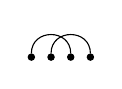
\begin{tikzpicture}[yscale=0.08,xscale=0.09,inner sep=.8pt,node distance=.25cm,>=latex']%,>=stealth',->]
\draw node [draw,circle,fill=black] (U1)               {};
\draw node [draw,circle,fill=black] [right of=U1] (U2) {};
\draw node [draw,circle,fill=black] [right of=U2] (U3) {};
\draw node [draw,circle,fill=black] [right of=U3] (U4) {};
\draw [] (U1.north) .. controls ($ (U1.north) + (0,4) $) and ($ (U3.north) + (0,4) $) .. (U3.north);
\draw [] (U2.north) .. controls ($ (U2.north) + (0,4) $) and ($ (U4.north) + (0,4) $) .. (U4.north);
\end{tikzpicture}
}% end \Crossing

\newcommand{\LabeledCrossingLL}[5]{%
\begin{tikzpicture}[scale=#1,inner sep=.8pt,node distance=.45cm,>=latex',
                    text height=1.5ex,text depth=.25ex]
\draw node [] (U1)               {#2};
\draw node [] [right of=U1] (U2) {#3};
\draw node [] [right of=U2] (U3) {#4};
\draw node [] [right of=U3] (U4) {#5};
\draw [->] (U1.north) .. controls ($ (U1.north) + (0,1.5) $) and ($ (U3.north) + (0,1.5) $) .. (U3.north);
\draw [->] (U2.north) .. controls ($ (U2.north) + (0,1.5) $) and ($ (U4.north) + (0,1.5) $) .. (U4.north);
\end{tikzpicture}
}% end \LabeledCrossingLL

\newcommand{\CrossingLL}{%
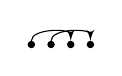
\begin{tikzpicture}[yscale=0.08,xscale=0.09,inner sep=.8pt,node distance=.25cm,>=latex']%,>=stealth',->]
\draw node [draw,circle,fill=black] (U1)               {};
\draw node [draw,circle,fill=black] [right of=U1] (U2) {};
\draw node [draw,circle,fill=black] [right of=U2] (U3) {};
\draw node [draw,circle,fill=black] [right of=U3] (U4) {};
\draw [->] (U1.north) .. controls ($ (U1.north) + (0,2) $) and ($ (U3.north) + (0,2) $) .. (U3.north);
\draw [->] (U2.north) .. controls ($ (U2.north) + (0,2) $) and ($ (U4.north) + (0,2) $) .. (U4.north);
\end{tikzpicture}
}% end \CrossingLL

\newcommand{\LabeledCrossingLR}[5]{%
\begin{tikzpicture}[scale=#1,inner sep=.8pt,node distance=.45cm,>=latex',
                    text height=1.5ex,text depth=.25ex]
\draw node [] (U1)               {#2};
\draw node [] [right of=U1] (U2) {#3};
\draw node [] [right of=U2] (U3) {#4};
\draw node [] [right of=U3] (U4) {#5};
\draw [->] (U1.north) .. controls ($ (U1.north) + (0,1.5) $) and ($ (U3.north) + (0,1.5) $) .. (U3.north);
\draw [<-] (U2.north) .. controls ($ (U2.north) + (0,1.5) $) and ($ (U4.north) + (0,1.5) $) .. (U4.north);
\end{tikzpicture}
}% end \LabeledCrossingLR

\newcommand{\CrossingLR}{%
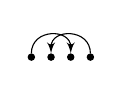
\begin{tikzpicture}[yscale=0.08,xscale=0.09,inner sep=.8pt,node distance=.25cm,>=latex']%,>=stealth',->]
\draw node [draw,circle,fill=black] (U1)               {};
\draw node [draw,circle,fill=black] [right of=U1] (U2) {};
\draw node [draw,circle,fill=black] [right of=U2] (U3) {};
\draw node [draw,circle,fill=black] [right of=U3] (U4) {};
\draw [->] (U1.north) .. controls ($ (U1.north) + (0,4) $) and ($ (U3.north) + (0,4) $) .. (U3.north);
\draw [<-] (U2.north) .. controls ($ (U2.north) + (0,4) $) and ($ (U4.north) + (0,4) $) .. (U4.north);
\end{tikzpicture}
}% end \CrossingLR

\newcommand{\LabeledCrossingRL}[5]{%
\begin{tikzpicture}[scale=#1,inner sep=.8pt,node distance=.45cm,>=latex',
                    text height=1.5ex,text depth=.25ex]
\draw node [] (U1)               {#2};
\draw node [] [right of=U1] (U2) {#3};
\draw node [] [right of=U2] (U3) {#4};
\draw node [] [right of=U3] (U4) {#5};
\draw [<-] (U1.north) .. controls ($ (U1.north) + (0,1.5) $) and ($ (U3.north) + (0,1.5) $) .. (U3.north);
\draw [->] (U2.north) .. controls ($ (U2.north) + (0,1.5) $) and ($ (U4.north) + (0,1.5) $) .. (U4.north);
\end{tikzpicture}
}% end \LabeledCrossingRL

\newcommand{\CrossingRL}{%
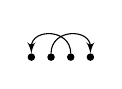
\begin{tikzpicture}[yscale=0.08,xscale=0.09,inner sep=.8pt,node distance=.25cm,>=latex']%,>=stealth',->]
\draw node [draw,circle,fill=black] (U1)               {};
\draw node [draw,circle,fill=black] [right of=U1] (U2) {};
\draw node [draw,circle,fill=black] [right of=U2] (U3) {};
\draw node [draw,circle,fill=black] [right of=U3] (U4) {};
\draw [<-] (U1.north) .. controls ($ (U1.north) + (0,4) $) and ($ (U3.north) + (0,4) $) .. (U3.north);
\draw [->] (U2.north) .. controls ($ (U2.north) + (0,4) $) and ($ (U4.north) + (0,4) $) .. (U4.north);
\end{tikzpicture}
}% end \CrossingRL

\newcommand{\LabeledCrossingRR}[5]{%
\begin{tikzpicture}[scale=#1,inner sep=.8pt,node distance=.45cm,>=latex',
                    text height=1.5ex,text depth=.25ex]
\draw node [] (U1)               {#2};
\draw node [] [right of=U1] (U2) {#3};
\draw node [] [right of=U2] (U3) {#4};
\draw node [] [right of=U3] (U4) {#5};
\draw [<-] (U1.north) .. controls ($ (U1.north) + (0,1.5) $) and ($ (U3.north) + (0,1.5) $) .. (U3.north);
\draw [<-] (U2.north) .. controls ($ (U2.north) + (0,1.5) $) and ($ (U4.north) + (0,1.5) $) .. (U4.north);
\end{tikzpicture}
}% end \LabeledCrossingRR

\newcommand{\CrossingRR}{%
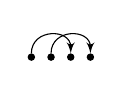
\begin{tikzpicture}[yscale=0.08,xscale=0.09,inner sep=.8pt,node distance=.25cm,>=latex']%,>=stealth',->]
\draw node [draw,circle,fill=black] (U1)               {};
\draw node [draw,circle,fill=black] [right of=U1] (U2) {};
\draw node [draw,circle,fill=black] [right of=U2] (U3) {};
\draw node [draw,circle,fill=black] [right of=U3] (U4) {};
\draw [->] (U1.north) .. controls ($ (U1.north) + (0,4) $) and ($ (U3.north) + (0,4) $) .. (U3.north);
\draw [->] (U2.north) .. controls ($ (U2.north) + (0,4) $) and ($ (U4.north) + (0,4) $) .. (U4.north);
\end{tikzpicture}
}% end \CrossingRR

\newcommand{\Inclusion}{%
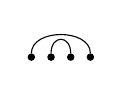
\begin{tikzpicture}[yscale=0.08,xscale=0.09,inner sep=.8pt,node distance=.25cm,>=latex']
\draw node [draw,circle,fill=black] (U1)               {};
\draw node [draw,circle,fill=black] [right of=U1] (U2) {};
\draw node [draw,circle,fill=black] [right of=U2] (U3) {};
\draw node [draw,circle,fill=black] [right of=U3] (U4) {};
\draw [] (U1.north) .. controls ($ (U1.north) + (0,4) $) and ($ (U4.north) + (0,4) $) .. (U4.north);
\draw [] (U2.north) .. controls ($ (U2.north) + (0,3) $) and ($ (U3.north) + (0,3) $) .. (U3.north);
\end{tikzpicture}
}% end \Inclusion

\newcommand{\LabeledInclusionLL}[5]{%
\begin{tikzpicture}[scale=#1,inner sep=.8pt,node distance=.45cm,>=latex',
                    text height=1.5ex,text depth=.25ex]
\draw node [] (U1)               {#2};
\draw node [] [right of=U1] (U2) {#3};
\draw node [] [right of=U2] (U3) {#4};
\draw node [] [right of=U3] (U4) {#5};
\draw [->] (U1.north) .. controls ($ (U1.north) + (0,2) $) and ($ (U4.north) + (0,2) $) .. (U4.north);
\draw [->] (U2.north) .. controls ($ (U2.north) + (0,1) $) and ($ (U3.north) + (0,1) $) .. (U3.north);
\end{tikzpicture}
}% end \LabeledInclusionLL

\newcommand{\InclusionLL}{%
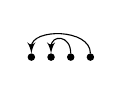
\begin{tikzpicture}[yscale=0.08,xscale=0.09,inner sep=.8pt,node distance=.25cm,>=latex']
\draw node [draw,circle,fill=black] (U1)               {};
\draw node [draw,circle,fill=black] [right of=U1] (U2) {};
\draw node [draw,circle,fill=black] [right of=U2] (U3) {};
\draw node [draw,circle,fill=black] [right of=U3] (U4) {};
+\draw [->] (U4.north) .. controls ($ (U4.north) + (0,4) $) and ($ (U1.north) + (0,4) $) .. (U1.north);
+\draw [->] (U3.north) .. controls ($ (U3.north) + (0,3) $) and ($ (U2.north) + (0,3) $) .. (U2.north);
\end{tikzpicture}
}% end \InclusionLL

\newcommand{\LabeledInclusionLR}[5]{%
\begin{tikzpicture}[scale=#1,inner sep=.8pt,node distance=.45cm,>=latex',
                    text height=1.5ex,text depth=.25ex]
\draw node [] (U1)               {#2};
\draw node [] [right of=U1] (U2) {#3};
\draw node [] [right of=U2] (U3) {#4};
\draw node [] [right of=U3] (U4) {#5};
\draw [->] (U1.north) .. controls ($ (U1.north) + (0,2) $) and ($ (U4.north) + (0,2) $) .. (U4.north);
\draw [<-] (U2.north) .. controls ($ (U2.north) + (0,1) $) and ($ (U3.north) + (0,1) $) .. (U3.north);
\end{tikzpicture}
}% end \LabeledInclusionLR

\newcommand{\InclusionLR}{%
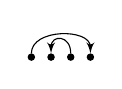
\begin{tikzpicture}[yscale=0.08,xscale=0.09,inner sep=.8pt,node distance=.25cm,>=latex']
\draw node [draw,circle,fill=black] (U1)               {};
\draw node [draw,circle,fill=black] [right of=U1] (U2) {};
\draw node [draw,circle,fill=black] [right of=U2] (U3) {};
\draw node [draw,circle,fill=black] [right of=U3] (U4) {};
\draw [->] (U1.north) .. controls ($ (U1.north) + (0,4) $) and ($ (U4.north) + (0,4) $) .. (U4.north);
\draw [<-] (U2.north) .. controls ($ (U2.north) + (0,3) $) and ($ (U3.north) + (0,3) $) .. (U3.north);
\end{tikzpicture}
}% end \InclusionLR

\newcommand{\LabeledInclusionRL}[5]{%
\begin{tikzpicture}[scale=#1,inner sep=.8pt,node distance=.45cm,>=latex',
                    text height=1.5ex,text depth=.25ex]
\draw node [] (U1)               {#2};
\draw node [] [right of=U1] (U2) {#3};
\draw node [] [right of=U2] (U3) {#4};
\draw node [] [right of=U3] (U4) {#5};
\draw [<-] (U1.north) .. controls ($ (U1.north) + (0,2) $) and ($ (U4.north) + (0,2) $) .. (U4.north);
\draw [->] (U2.north) .. controls ($ (U2.north) + (0,1) $) and ($ (U3.north) + (0,1) $) .. (U3.north);
\end{tikzpicture}
}% end \LabeledInclusionRL

\newcommand{\InclusionRL}{%
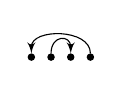
\begin{tikzpicture}[yscale=0.08,xscale=0.09,inner sep=.8pt,node distance=.25cm,>=latex']
\draw node [draw,circle,fill=black] (U1)               {};
\draw node [draw,circle,fill=black] [right of=U1] (U2) {};
\draw node [draw,circle,fill=black] [right of=U2] (U3) {};
\draw node [draw,circle,fill=black] [right of=U3] (U4) {};
\draw [<-] (U1.north) .. controls ($ (U1.north) + (0,4) $) and ($ (U4.north) + (0,4) $) .. (U4.north);
\draw [->] (U2.north) .. controls ($ (U2.north) + (0,3) $) and ($ (U3.north) + (0,3) $) .. (U3.north);
\end{tikzpicture}
}% end \InclusionRL

\newcommand{\LabeledInclusionRR}[5]{%
\begin{tikzpicture}[scale=#1,inner sep=.8pt,node distance=.45cm,>=latex',
                    text height=1.5ex,text depth=.25ex]
\draw node [] (U1)               {#2};
\draw node [] [right of=U1] (U2) {#3};
\draw node [] [right of=U2] (U3) {#4};
\draw node [] [right of=U3] (U4) {#5};
\draw [<-] (U1.north) .. controls ($ (U1.north) + (0,2) $) and ($ (U4.north) + (0,2) $) .. (U4.north);
\draw [<-] (U2.north) .. controls ($ (U2.north) + (0,1) $) and ($ (U3.north) + (0,1) $) .. (U3.north);
\end{tikzpicture}
}% end \LabeledInclusionRR

\newcommand{\InclusionRR}{%
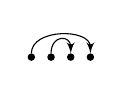
\begin{tikzpicture}[yscale=0.08,xscale=0.09,inner sep=.8pt,node distance=.25cm,>=latex']
\draw node [draw,circle,fill=black] (U1)               {};
\draw node [draw,circle,fill=black] [right of=U1] (U2) {};
\draw node [draw,circle,fill=black] [right of=U2] (U3) {};
\draw node [draw,circle,fill=black] [right of=U3] (U4) {};
\draw [->] (U1.north) .. controls ($ (U1.north) + (0,4) $) and ($ (U4.north) + (0,4) $) .. (U4.north);
\draw [->] (U2.north) .. controls ($ (U2.north) + (0,3) $) and ($ (U3.north) + (0,3) $) .. (U3.north);
\end{tikzpicture}
}% end \InclusionRR

\newcommand{\Precedence}{%

\begin{tikzpicture}[yscale=0.08,xscale=0.09,inner sep=.8pt,node distance=.25cm,>=latex']
\draw node [draw,circle,fill=black] (U1)               {};
\draw node [draw,circle,fill=black] [right of=U1] (U2) {};
\draw node [draw,circle,fill=black] [right of=U2] (U3) {};
\draw node [draw,circle,fill=black] [right of=U3] (U4) {};
\draw [] (U1.north) .. controls ($ (U1.north) + (0,4) $) and ($ (U2.north) + (0,4) $) .. (U2.north);
\draw [] (U3.north) .. controls ($ (U3.north) + (0,4) $) and ($ (U4.north) + (0,4) $) .. (U4.north);
\end{tikzpicture}
}% end \Precedence

\newcommand{\LabeledPrecedenceLL}[5]{%
\begin{tikzpicture}[scale=#1,inner sep=.8pt,node distance=.45cm,>=latex',
                    text height=1.5ex,text depth=.25ex]
\draw node [] (U1)               {#2};
\draw node [] [right of=U1] (U2) {#3};
\draw node [] [right of=U2] (U3) {#4};
\draw node [] [right of=U3] (U4) {#5};
\draw [->] (U1.north) .. controls ($ (U1.north) + (0,1.5) $) and ($ (U2.north) + (0,1.5) $) .. (U2.north);
\draw [->] (U3.north) .. controls ($ (U3.north) + (0,1.5) $) and ($ (U4.north) + (0,1.5) $) .. (U4.north);
\end{tikzpicture}
}% end \PrecedenceLL

\newcommand{\PrecedenceLL}{%
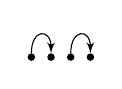
\begin{tikzpicture}[yscale=0.08,xscale=0.09,inner sep=.8pt,node distance=.25cm,>=latex']
\draw node [draw,circle,fill=black] (U1)               {};
\draw node [draw,circle,fill=black] [right of=U1] (U2) {};
\draw node [draw,circle,fill=black] [right of=U2] (U3) {};
\draw node [draw,circle,fill=black] [right of=U3] (U4) {};
\draw [->] (U1.north) .. controls ($ (U1.north) + (0,4) $) and ($ (U2.north) + (0,4) $) .. (U2.north);
\draw [->] (U3.north) .. controls ($ (U3.north) + (0,4) $) and ($ (U4.north) + (0,4) $) .. (U4.north);
\end{tikzpicture}
}% end \PrecedenceLL

\newcommand{\LabeledPrecedenceLR}[5]{%
\begin{tikzpicture}[scale=#1,inner sep=.8pt,node distance=.45cm,>=latex',
                    text height=1.5ex,text depth=.25ex]
\draw node [] (U1)               {#2};
\draw node [] [right of=U1] (U2) {#3};
\draw node [] [right of=U2] (U3) {#4};
\draw node [] [right of=U3] (U4) {#5};
\draw [->] (U1.north) .. controls ($ (U1.north) + (0,1.5) $) and ($ (U2.north) + (0,1.5) $) .. (U2.north);
\draw [<-] (U3.north) .. controls ($ (U3.north) + (0,1.5) $) and ($ (U4.north) + (0,1.5) $) .. (U4.north);
\end{tikzpicture}
}% end \PrecedenceLR

\newcommand{\PrecedenceLR}{%
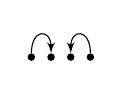
\begin{tikzpicture}[yscale=0.08,xscale=0.09,inner sep=.8pt,node distance=.25cm,>=latex']
\draw node [draw,circle,fill=black] (U1)               {};
\draw node [draw,circle,fill=black] [right of=U1] (U2) {};
\draw node [draw,circle,fill=black] [right of=U2] (U3) {};
\draw node [draw,circle,fill=black] [right of=U3] (U4) {};
\draw [->] (U1.north) .. controls ($ (U1.north) + (0,4) $) and ($ (U2.north) + (0,4) $) .. (U2.north);
\draw [<-] (U3.north) .. controls ($ (U3.north) + (0,4) $) and ($ (U4.north) + (0,4) $) .. (U4.north);
\end{tikzpicture}
}% end \PrecedenceLR

\newcommand{\LabeledPrecedenceRL}[5]{%
\begin{tikzpicture}[scale=#1,inner sep=.8pt,node distance=.45cm,>=latex',
                    text height=1.5ex,text depth=.25ex]
\draw node [] (U1)               {#2};
\draw node [] [right of=U1] (U2) {#3};
\draw node [] [right of=U2] (U3) {#4};
\draw node [] [right of=U3] (U4) {#5};
\draw [<-] (U1.north) .. controls ($ (U1.north) + (0,1.5) $) and ($ (U2.north) + (0,1.5) $) .. (U2.north);
\draw [->] (U3.north) .. controls ($ (U3.north) + (0,1.5) $) and ($ (U4.north) + (0,1.5) $) .. (U4.north);
\end{tikzpicture}
}% end \PrecedenceRL

\newcommand{\PrecedenceRL}{%
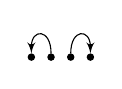
\begin{tikzpicture}[yscale=0.08,xscale=0.09,inner sep=.8pt,node distance=.25cm,>=latex']
\draw node [draw,circle,fill=black] (U1)               {};
\draw node [draw,circle,fill=black] [right of=U1] (U2) {};
\draw node [draw,circle,fill=black] [right of=U2] (U3) {};
\draw node [draw,circle,fill=black] [right of=U3] (U4) {};
\draw [<-] (U1.north) .. controls ($ (U1.north) + (0,4) $) and ($ (U2.north) + (0,4) $) .. (U2.north);
\draw [->] (U3.north) .. controls ($ (U3.north) + (0,4) $) and ($ (U4.north) + (0,4) $) .. (U4.north);
\end{tikzpicture}
}% end \PrecedenceRL

\newcommand{\LabeledPrecedenceRR}[5]{%
\begin{tikzpicture}[scale=#1,inner sep=.8pt,node distance=.45cm,>=latex',
                    text height=1.5ex,text depth=.25ex]
\draw node [] (U1)               {#2};
\draw node [] [right of=U1] (U2) {#3};
\draw node [] [right of=U2] (U3) {#4};
\draw node [] [right of=U3] (U4) {#5};
\draw [<-] (U1.north) .. controls ($ (U1.north) + (0,1.5) $) and ($ (U2.north) + (0,1.5) $) .. (U2.north);
\draw [<-] (U3.north) .. controls ($ (U3.north) + (0,1.5) $) and ($ (U4.north) + (0,1.5) $) .. (U4.north);
\end{tikzpicture}
}% end \PrecedenceRR

\newcommand{\PrecedenceRR}{%
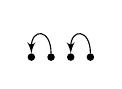
\begin{tikzpicture}[yscale=0.08,xscale=0.09,inner sep=.8pt,node distance=.25cm,>=latex']
\draw node [draw,circle,fill=black] (U1)               {};
\draw node [draw,circle,fill=black] [right of=U1] (U2) {};
\draw node [draw,circle,fill=black] [right of=U2] (U3) {};
\draw node [draw,circle,fill=black] [right of=U3] (U4) {};
\draw [<-] (U1.north) .. controls ($ (U1.north) + (0,4) $) and ($ (U2.north) + (0,4) $) .. (U2.north);
\draw [<-] (U3.north) .. controls ($ (U3.north) + (0,4) $) and ($ (U4.north) + (0,4) $) .. (U4.north);
\end{tikzpicture}
}% end \PrecedenceRR

%%%%%%%%%%%%%%%%%%%%%%%%%%%%%%%%%%%%%%%%%%%%%%%%%%%%%%%%%%%%%%%%%%%%%%%%%%%%%%%

\newtheorem{fact}{Fact}

%%%%%%%%%%%%%%%%%%%%%%%%%%%%%%%%%%%%%%%%%%%%%%%%%%%%%%%%%%%%%%%%%%%%%%%%%%%%%%%

\makeatletter
\newcommand{\pushright}[1]{\ifmeasuring@#1\else\omit\hfill$\displaystyle#1$\fi\ignorespaces}
\newcommand{\pushleft}[1]{\ifmeasuring@#1\else\omit$\displaystyle#1$\hfill\fi\ignorespaces}
\makeatother

%%%%%%%%%%%%%%%%%%%%%%%%%%%%%%%%%%%%%%%%%%%%%%%%%%%%%%%%%%%%%%%%%%%%%%%%%%%%%%%

\begin{document}

%%%%%%%%%%%%%%%%%%%%%%%%%%%%%%%%%%%%%%%%%%%%%%%%%%%%%%%%%%%%%%%%%%%%%%%%%%%%%%%

\title{%
Unshuffling Permutations}%

\author{%
  Samuele Giraudo \and
  St\'ephane Vialette
}% end author
\institute{%
  Universit\'e Paris-Est, LIGM (UMR 8049), CNRS, UPEM, ESIEE Paris, ENPC,
  F-77454, Marne-la-Vallée, France\\
  \email{samuele.giraudo@univ-mlv.fr} \\
  \email{vialette@univ-mlv.fr}
}% end institute
\date{\today}

\maketitle

%%%%%%%%%%%%%%%%%%%%%%%%%%%%%%%%%%%%%%%%%%%%%%%%%%%%%%%%%%%%%%%%%%%%%%%%%%%%%%%

\begin{abstract}
    A permutation is said to be a square if it can be obtained by
    shuffling two order-isomorphic patterns. The definition is intended
    to be the natural counterpart to the ordinary shuffle of words and
    languages. In this paper, we tackle the problem of recognizing square
    permutations from both the point of view of algebra and algorithmic.
    On the one hand, we present some algebraic and combinatorial
    properties of the shuffle product of permutations. We follow an
    unusual line consisting in defining the shuffle of permutations by
    means of an unshuffling operator, known as a coproduct. This
    strategy allows to obtain easy proofs for algebraic and combinatorial
    properties of our shuffle product. We besides exhibit a bijection
    between square $(213,231)$-avoiding permutations and square binary
    words. On the other hand, we prove that recognizing square
    permutations is \NPC. \sout{This property is proved by establishing a
    reduction from the pattern involvement problem and by using a
    containment-free perfect matching criterion to decide if a
    permutation is a square.}
    \uline{This property is proved by establishing a
    reduction from the pattern involvement problem and by using a
    contrained oriented perfect matching criterion to decide if a
    permutation is a square.}
\end{abstract}

%%%%%%%%%%%%%%%%%%%%%%%%%%%%%%%%%%%%%%%%%%%%%%%%%%%%%%%%%%%%%%%%%%%%%%%%%%%%%%%

%%
%%
%% ---- Introduction ----
%%
\section{Introduction}
\label{section:Introduction}
The \emph{shuffle product} $\shuffle$ is a very famous operation on words
first defined by Eilenberg and Mac Lane~\cite{Eilenberg:MacLane:1953}.
Given three words $u$, $v_1$, and $v_2$, $u$ is said to be a \emph{shuffle}
of $v_1$ and $v_2$ if it can be formed by interleaving the letters from
$v_1$ and $v_2$ in a way that maintains the left-to-right ordering of the
letters from each word. In addition to purely combinatorial questions,
the shuffle product of words leads to the following computational ones:
\begin{enumerate}
    \item \label{item:problem_1}
    Given two words $v_1$ and $v_2$, compute the set $v_1 \shuffle v_2$.
    \item \label{item:problem_2}
    Given three words $u$, $v_1$, and $v_2$, decide if $u$ is a shuffle
    of $v_1$ and $v_2$.
    \item \label{item:problem_3}
    Given words $u$, $v_1$, \dots, $v_k$, decide if $u$ is in
    $v_1 \shuffle \dots \shuffle v_k$.
    \item \label{item:problem_4}
    Given a word $u$, decide if there is a word $v$ such that $u$ is
    in $v \shuffle v$.
\end{enumerate}
Even if these problems seem similar, they are very different in terms
of complexity. Let us now review some facts about these. In what follows,
$n$ denotes the size of $u$ and $m_i$ denotes the size of each $v_i$.
A solution to Problem~\ref{item:problem_1} can be computed in
\begin{equation}
    O\left((m_1 + m_2) \; \binom{m_1 + m_2}{m_1}\right)
\end{equation}
time~\cite{Spehner:TCS:1986}. An improvement and a generalization
of~Problem~\ref{item:problem_1} has been proposed
in~\cite{Allauzen:IGM:2000}, where it is proved that given words
$v_1$, \dots, $v_k$, the iterated shuffle
$v_1 \shuffle \dots \shuffle v_k$ can be computed in
\begin{equation}
    O\left(\binom{m_1 + \dots + m_k}{m_1, \dots, m_k}\right)
\end{equation}
time. Problem~\ref{item:problem_2} is in \Pclass; it is indeed a
classical textbook exercise to design an efficient dynamic programming
algorithm solving it. It can be tested in $O\left(n^2 / \log(n)\right)$
time~\cite{Leeuwen:Nivat:IPL:1982}. To the best of our knowledge, the
first $O(n^2)$ time algorithm for this problem appeared
in~\cite{Mansfield:DAM:1983}. This algorithm can easily be extended to
check in polynomial-time whether or not a word is in the shuffle of any
fixed number of given words. Nevertheless, Problem~\ref{item:problem_3}
is \NPC~\cite{Mansfield:DAM:1983,Warmuth:Haussler:JCSS:1984}. This
remains true even if the ground alphabet has size
$3$~\cite{Warmuth:Haussler:JCSS:1984}. Of particular interest,
it is shown in~\cite{Warmuth:Haussler:JCSS:1984} that
Problem~\ref{item:problem_3} remains \NPC even if all the words $v_i$,
$i \in [k]$, are identical, thereby proving that, for two words $u$ and
$v$, it is \NPC to decide whether or not $u$ is in the iterated shuffle
of $v$. Again, this remains true even if the ground alphabet has size $3$.
Let us now finally focus on Problem~\ref{item:problem_4}. It is shown
in~\cite{Buss:Soltys:2014,Rizzi:Vialette:CSR:2013} that it is \NPC to
decide if a word $u$ is a \emph{square} (w.r.t. the shuffle), that is
a word $u$ with the property that there exists a word $v$ such that $u$
is a shuffle of $v$ with itself. Hence, Problem~\ref{item:problem_4}
is \NPC.
\smallskip

This paper is intended to study a natural generalization of $\shuffle$,
denoted by $\SHUFFLE$, as a shuffle of permutations. Roughly speaking,
given three permutations $\pi$, $\sigma_1$, and $\sigma_2$, $\pi$ is
said to be a \emph{shuffle} of $\sigma_1$ and $\sigma_2$ if $\pi$ (viewed
as a word) is a shuffle of two words that are order-isomorphic to
$\sigma_1$ and $\sigma_2$. Our intention in this paper is to study this
shuffle product of permutations $\SHUFFLE$ both from a combinatorial and
from a computational point of view by focusing on \emph{square}
permutations, that are permutations $\pi$ being in the shuffle of a
permutation $\sigma$ with itself. The shuffle product defined and
considered in this paper is different from other existing and well-known
shuffle products on permutations. For instance, in~\cite{DHT:IJAC:2002},
the authors define the \emph{shifted shuffle product}. For this product,
$\pi$ is a shuffle of $\sigma_1$ and $\sigma_2$ if $\pi$ is in the
shuffle, as words, of $\sigma_1$ and the word obtained by incrementing
all the letters of $\sigma_2$ by the size of $\sigma_1$. It is a simple
exercise to prove that, given three permutations $\pi$, $\sigma_1$, and
$\sigma_2$, deciding if $\pi$ is a in the shifted shuffle of $\sigma_1$
and $\sigma_2$ is in~\Pclass.
\smallskip

This paper is organized as follows. In
Section~\ref{section:Shuffle product on permutations} we provide a
precise definition of $\SHUFFLE$. This definition passes through the
preliminary definition of an operator~$\Delta$, allowing to
\emph{unshuffle} permutations. This operator is in fact a coproduct,
endowing the linear span of all permutations with a coalgebra structure
(see~\cite{Joni:Rota:1979} or~\cite{Grinberg:Reiner:2014} for the
definition of these algebraic structures). By duality, the unshuffling
operator $\Delta$ leads to the definition of our shuffle operation on
permutations. This approach has many advantages. First, some
combinatorial properties of $\SHUFFLE$ depend on properties of $\Delta$
and are more easy to prove on the coproduct side. Second, this way of
doing allows to obtain a clear description of the multiplicities of the
elements appearing in the shuffle of two permutations, which are worthy
of interest from a combinatorial point of view.
Section~\ref{section:Binary square words and permutations} is devoted to
show that the problems related to the shuffle of words has links with
the shuffle of permutations. In particular, we show that binary words
that are square are in one-to-one correspondence with square
permutations avoiding some patterns
(Proposition~\ref{prop:bijection_binary_to_permutations_squares}). Next,
Section~\ref{section:Algebraic issues} presents some algebraic and
combinatorial properties of~$\SHUFFLE$. We show that $\SHUFFLE$ is
associative and commutative
(Proposition~\ref{prop:shuffle_associative_commutative}), and that if a
permutation is a square, its mirror, complement, and inverse are also
squares (Proposition~\ref{prop:square_stability}). Finally,
Section~\ref{section:Algorithmic issues} presents the most import result
of this paper: the fact that deciding if a permutation is a square is
\NPC (Proposition~\ref{proposition:hardness}). This result is obtained
by exhibiting a reduction from the pattern involvement
problem~\cite{Bose:Buss:Lubiw:1998} which is \NPC.

%%%%%%%%%%%%%%%%%%%%%%%%%%%%%%%%%%%%%%%%%%%%%%%%%%%%%%%%%%%%%%%%%%%%%%%%%%%%%%%

%%
%% ---- Notations ----
%%
\section{Notations}
\label{section:Notations}

If $S$ is a finite set, the cardinality of $S$ is denoted by $|S|$,
and if $P$ and $Q$ are two disjoint sets, $P \sqcup Q$ denotes the
disjoint union of $P$ and $Q$. For any nonnegative integer $n$, $[n]$
is the set $\{1, \dots, n\}$.

We follow the usual terminology on words~\cite{ChoffrutKarhumaki1997}.
Let us recall here the most important ones. Let $u$ be a word. The
length of $u$ is denoted by $|u|$. The \emph{empty word}, the only word
of null length, is denoted by $\epsilon$. We denote by $\widetilde{u}$
the \emph{mirror image} of $u$ that is the word
$u_{|u|} u_{|u| - 1} \dots u_1$. If $P$ is a subset of $[|u|]$, $u_{|P}$
is the subword of $u$ consisting in the letters of $u$ at the positions
specified by the elements of $P$. If $u$ is a word of integers and $k$
is an integer, we denote by $u[k]$ the word obtained by incrementing by
$k$ all letters of $u$. The \emph{shuffle} of two words $u$ and $v$ is
the set recursively defined by
$u \shuffle \epsilon = u = \epsilon \shuffle u$ and
$ua \shuffle vb = (u \shuffle vb)a \cup (ua \shuffle v)b$, were $a$ and
$b$ are letters. A word $u$ is a \emph{square} if there exists a word $v$
such that $u$ belongs to $v \shuffle v$.

We denote by $S_n$ the set of permutations of size $n$ and by $S$ the
set of all permutations. In this paper, permutations of a size $n$ are
specified by words of length $n$ on the alphabet $[n]$ and without
multiple occurrence of a letter, so that all above definitions about
words remain valid on permutations. The only difference lies on the
fact that we shall denote by $\pi(i)$ (instead of $\pi_i$) the $i$-th
letter of any permutation $\pi$. For any nonnegative integer $n$, we
write $\nearrow_{n}$ (resp. $\searrow_{n}$) for the permutation
$1 2 \dots n$ (resp. $n (n-1) \dots 1$). If $\pi$ is a permutation of
$S_n$, we denote by $\bar \pi$ the \emph{complementary} of $\pi$ that is
the permutation satisfying $\bar \pi(i) = n - \pi(i) + 1$ for all
$i \in [n]$. The \emph{inverse} of $\pi$ is denoted by $\pi^{-1}$.

If $u$ is a word of integers without multiple occurrences of a same
letter, $\STD(u)$ is the \emph{standarized} of $u$, that is the unique
permutation of the same size as $u$ such that for all $i, j \in [|u|]$,
$u_i < u_j$ if and only if $\STD(u)(i) < \STD(u)(j)$. In particular, the
image of the map $\STD$ is the set $S$ of all permutations. Two words $u$
and $v$ having the same standarized are \emph{order-isomorphic}. If
$\sigma$ is a permutation, there is an \emph{occurrence} of (the
\emph{pattern}) $\sigma$ in $\pi$ if there is a set $P$ of indexes of
letters of $\pi$ such that $\sigma$ and $\pi_{|P}$ are order-isomorphic.
When $\pi$ does not admit any occurrence of $\sigma$, $\pi$ \emph{avoids}
$\sigma$.

Let us now provide some definitions about graphs and \uline{oriented}
matching, used in the sequel.
For a graph $G$, we denote $\VS{G}$ as the set of vertices
and $\ES{G}$ as the set of edges of $G$. Let $u = u_1 u_2 \dots u_n$ be
a word. The \emph{clique graph associated to $u$}, denoted by $K_u$, is
the complete graph on $\VS{K_u} = \{u_1, u_2, \ldots, u_n\}$. The
structure of this underlying graph is linear, \emph{i.e.}, the set of
its vertices is equipped with a natural total order $<$ defined by
$u_i < u_j$ if and only if $i < j$. For a linear graph, we write
$(u_i, u_j)$ instead of $\{u_i, u_j\}$ for an edge if it is clear from
the context that $i < j$. Recall that two edges of a graph are
\emph{independent} if they do not share a common vertex, and that a
\emph{matching} $\mathcal{M}$ in $G$ is a set of pairwise independent
edges. A matching is \emph{perfect} if it covers all the vertices of the
graph.
\sout{In case the set of vertices is equipped with a total order, a
matching $\mathcal{M}$ is said to be \emph{containment-free} if there do
not exist (independent) edges $(u_i, u_j)$ and $(u_k, u_\ell)$ in
$\mathcal{M}$ such that $u_i < u_k < u_\ell < u_j$ or
$u_k < u_i < u_j < u_\ell$.}
An \emph{oriented matching}
$\vv{\mathcal{M}}$ of $\mathcal{M}$ is a directed matching obtained
from $\mathcal{M}$ by orienting its edges.
\textbf{D\'efinir l'inclusion de motifs. En fait, je pense même qu'il ne faudrait
parler que de graphes orientés. Qu'en penses-tu?}


%%%%%%%%%%%%%%%%%%%%%%%%%%%%%%%%%%%%%%%%%%%%%%%%%%%%%%%%%%%%%%%%%%%%%%%%%%%%%%%

%%
%% ---- Shuffle product on permutations ----
%%
\section{Shuffle product on permutations}
\label{section:Shuffle product on permutations}

The purpose of this section is to define a shuffle product $\SHUFFLE$
on permutations. To define this shuffle product, we shall first define
a coproduct denoted by $\Delta$, enabling to unshuffle permutations.
By duality, $\Delta$ implies the definition of $\SHUFFLE$. The reason
why we need to pass by the definition of $\Delta$ to define $\SHUFFLE$
is justified by the fact that a lot of properties of $\SHUFFLE$ depend
of properties of $\Delta$ and that this strategy allows to write concise
and clear proofs of them. We invite the reader unfamiliar with the
concepts of coproduct and duality to consult~\cite{Joni:Rota:1979}
or~\cite{Grinberg:Reiner:2014}.
\medskip

Let use denote by $\QQ[S]$ the linear span of all permutations. We
define a linear coproduct $\Delta$ on $\QQ[S]$ in the following way. For
any permutation $\pi$, we set
\begin{equation} \label{equ:unshuffling_coproduct}
    \Delta(\pi) =
    \sum_{P_1 \sqcup P_2 = [|\pi|]}
    \STD\left(\pi_{|P_1}\right) \otimes \STD\left(\pi_{|P_2}\right).
\end{equation}
We call $\Delta$ the \emph{unshuffling coproduct of permutations}. For
instance,
\begin{equation}
    \Delta(213) =
    \epsilon \otimes 213 + 2. 1 \otimes 12 +
    1 \otimes 21 + 2. 12 \otimes 1 + 21 \otimes 1 + 213 \otimes \epsilon,
\end{equation}
\begin{equation}
    \Delta(1234) =
    \epsilon \otimes 1234 + 4. 1 \otimes 123 + 6. 12 \otimes 12 +
    4. 123 \otimes 1 + 1234 \otimes \epsilon,
\end{equation}
\begin{equation}\begin{split} \label{equ:example_unshuffling_coproduct}
    \Delta(1432) & =
    \epsilon \otimes 1432 + 3. {\bf 1 \otimes 132} + 1 \otimes 321 +
    3. 12 \otimes 21 \\ & + 3. 21 \otimes 12 + 3. 132 \otimes 1 +
    321 \otimes 1 + 1432 \otimes \epsilon.
\end{split}\end{equation}
Observe that the coefficient of the tensor $1 \otimes 132$ is $3$
in~\eqref{equ:example_unshuffling_coproduct} because there are exactly
three ways to extract from the permutation $1432$ two disjoint subwords
respectively order-isomorphic to the permutations $1$ and $132$.
\medskip

As announced, let us now use $\Delta$ to define a shuffle product on
permutations. As any coproduct, $\Delta$ leads to the definition of a
product obtained by duality in the following way.
From~\eqref{equ:unshuffling_coproduct}, for any permutation $\pi$, we
have
\begin{equation} \label{equ:schematic_coproduct}
    \Delta(\pi) =
    \sum_{\sigma, \nu \in S} \lambda_{\sigma, \nu}^\pi \;
    \sigma \otimes \nu,
\end{equation}
where the $\lambda_{\sigma, \nu}^\pi$ are nonnegative integers. Now,
by definition of duality, the dual product of $\Delta$, denoted by
$\SHUFFLE$, is a linear binary product on $\QQ[S]$. It satisfies, for
any permutations $\sigma$ and $\nu$,
\begin{equation}
    \sigma \SHUFFLE \nu =
    \sum_{\pi \in S}
    \lambda_{\sigma, \nu}^\pi \; \pi,
\end{equation}
where the coefficients $\lambda_{\sigma, \nu}^\pi$ are the ones
of~\eqref{equ:schematic_coproduct}. We call $\SHUFFLE$ the
\emph{shuffle product of permutations}. For instance,
\begin{equation}\begin{split} \label{equ:example_shuffle_product}
    12 \SHUFFLE 21 & =
    1243 + 1324 + 2.1342 + 2.1423 + 3. {\bf 1432} + 2134 + 2.2314 \\
    & + 3.2341 + 2413 + 2.2431 + 2.3124 + 3142 + 3.3214 + 2.3241 \\
    & + 3421 + 3.4123 + 2.4132 + 2.4213 + 4231 + 4312.
\end{split}\end{equation}
Observe that the coefficient $3$ of the permutation $1432$
in~\eqref{equ:example_shuffle_product} comes from the fact that the
coefficient of the tensor $12 \otimes 21$ is $3$
in~\eqref{equ:example_unshuffling_coproduct}.
\medskip

Intuitively, this product shuffles the values and the positions of the
letters of the permutations. As first and easy properties of $\SHUFFLE$,
one can observe that the empty permutation $\epsilon$ is a unit for
$\SHUFFLE$ and that this product is graded by the sizes of the
permutations (\emph{i.e.}, the product of a permutation of size $n$ with
a permutation of size $m$ produces a sum of permutations of size $n + m$).
Notice that there are other shuffle products on
permutations~\cite{DHT:IJAC:2002}: the \emph{shifted shuffle} and the
\emph{convolution product}. Our shuffle product is different from these
last two.
\medskip

We say that a permutation $\pi$ \emph{appears} in the shuffle
$\sigma \SHUFFLE \nu$ of two permutations $\sigma$ and $\nu$ if the
coefficient $\lambda_{\sigma, \nu}^\pi$ defined above is different from
zero. In a more combinatorial way, this is equivalent to say that there
are two sets $P_1$ and $P_2$ of disjoints indexes of letters of $\pi$
satisfying $P_1 \sqcup P_2 = [|\pi|]$ such that the subword $\pi_{|P_1}$
is order-isomorphic to $\sigma$ and the subword $\pi_{|P_2}$ is
order-isomorphic to $\nu$.
\medskip

Besides, a permutation $\pi$ is a \emph{square} if there is a
permutation $\sigma$ such that $\pi$ appears in $\sigma \SHUFFLE \sigma$.
In this case, we say that $\sigma$ is a \emph{square root} of $\pi$.
Equivalently, $\pi$ is a square with $\sigma$ as square root if and only
if in the expansion of $\Delta(\pi)$, there is a tensor
$\sigma \otimes \sigma$ with a nonzero coefficient. In a more
combinatorial way, this is equivalent to say that there are two sets
$P_1$ and $P_2$ of disjoints indexes of letters of $\pi$ satisfying
$P_1 \sqcup P_2 = [|\pi|]$ such that the subword $\pi_{|P_1}$ and
$\pi_{|P_2}$ are order-isomorphic. Computer experiments give us the
first numbers of square permutations with respects to their size, which
are, from size $0$ to $10$,
\begin{equation}
    1, 0, 2, 0, 20, 0, 504, 0, 21032, 0, 1293418.
\end{equation}
This sequence (and its subsequence obtained by removing the $0$s) is for
the time being not listed in~\cite{Slo}. The square permutations of
sizes $0$ to $4$ are
\smallskip

\begin{tabular}{c|c|c}
    Size $0$ \, & Size $2$ & Size $4$ \\ \hline
    \multirow{2}{*}{\, $\epsilon$} &
    \multirow{2}{*}{\, $12$, $21$ \,} &
    $1234$, $1243$, $1423$, $1324$, $1342$, $4132$, $3124$, $3142$,
    $3412$, $4312$, \\
    & & $2134$, $2143$, $2413$, $4213$, $2314$, $2431$, $4231$, $3241$,
    $3421$, $4321$
\end{tabular}
\medskip

%%%%%%%%%%%%%%%%%%%%%%%%%%%%%%%%%%%%%%%%%%%%%%%%%%%%%%%%%%%%%%%%%%%%%%%%%%%%%%%

%%
%% ---- Binary square words and permutations ----
%%
\section{Binary square words and permutations}
\label{section:Binary square words and permutations}
In this section, we shall show that the square binary words are in
one-to-one correspondence with square permutations avoiding some
patterns. This property establishes a link between the shuffle of binary
words and our shuffle of permutations and allows to obtain a new
description of square binary words.
\medskip

Let $u$ be a binary word of length $n$ with $k$ occurrences of $0$.
We denote by $\BINTOPERM$ the map sending any such word $u$ to the
permutation obtained by replacing from left to right each occurrence of
$0$ in $u$ by $1$, $2$, \dots, $k$, and from right to left each
occurrence of $1$ in $u$ by $k + 1$, $k + 2$, \dots, $n$. For instance,
\begin{equation}
    \BINTOPERM({\bf 1}00{\bf 1}0{\bf 1}{\bf 1}0{\bf 1}000) =
    {\bf C} 12 {\bf B} 3 {\bf A} {\bf 9} 4 {\bf 8} 567.
\end{equation}
Observe that for any nonempty permutation $\pi$ in the image of
$\BINTOPERM$, there is exactly one binary word $u$ such that
$\BINTOPERM(u0) = \BINTOPERM(u1) = \pi$. In support of this observation,
when $\pi$ has an even size, we denote by $\PERMTOBIN(\pi)$ the word $ua$
such that $|ua|_0$ and $|ua|_1$ are both even, where $a \in \{0, 1\}$.
\medskip

\begin{proposition} \label{prop:bijection_binary_to_permutations_squares}
    For any $n \geq 0$, the map $\BINTOPERM$ restricted to the set of
    square binary words of length $2n$ is a bijection between this last
    set and the set of square permutations of size $2n$ avoiding the
    patterns $213$ and $231$.
\end{proposition}
\begin{proof}
    [of Proposition~\ref{prop:bijection_binary_to_permutations_squares}]
    The statement of the proposition is a consequence of the
    following claims implying that $\PERMTOBIN$ is the inverse
    map of $\BINTOPERM$ over the set of square binary words.
    \begin{claim} \label{claim:binary_to_permutation_avoiding}
        The image of $\BINTOPERM$ is the set of all permutations
        avoiding $213$ and $231$.
    \end{claim}
    \begin{proof}[of Claim~\ref{claim:binary_to_permutation_avoiding}]
        Let us first show that the image of $\BINTOPERM$ contains only
        permutations avoiding $213$ and $231$. Let $u$ be a binary word,
        $\pi = \BINTOPERM(u)$, and $P_0$ (resp. $P_1$) be the set of the
        positions of the occurrences of $0$ (resp. $1$) in $u$. By
        definition of $\BINTOPERM$, from left to right, the subword
        $v = \pi_{|P_0}$ is increasing and the subword $w = \pi_{|P_1}$
        is decreasing, and all letters of $w$ are greater than those
        of~$v$. Now, assume that $\pi$ admits an occurrence of $213$.
        Then, since $v$ is increasing and $w$ is decreasing, there is an
        occurrence of $3$ (resp. $13$, $23$) in $v$ and a relative
        occurrence of $21$ (resp. $2$, $1$). All these three cases
        contradict the fact that all letters of $w$ are greater than
        those of $v$. A similar argument shows that $\pi$ avoids~$231$
        as well.
        \smallskip

        Finally, observe that any permutation $\pi$ avoiding $213$ and
        $231$ necessarily starts by the smallest possible letter or the
        greatest possible letter. This property is then true for the
        suffix of $\pi$ obtained by deleting its first letter,
        and so on for all of its suffixes. Thus, by
        replacing each letter $a$ of $\pi$ by $0$ (resp. $1$) if $a$ has the
        role of a smallest (resp. greatest) letter, one obtains a binary
        word $u$ such that $\BINTOPERM(u) = \pi$. Hence, all permutations
        avoiding $213$ and $231$ are in the image of $\BINTOPERM$.
        \qed
    \end{proof}
    \begin{claim} \label{claim:square_binary_to_square_permutation}
        If $u$ is a square binary word, $\BINTOPERM(u)$ is a square
        permutation.
    \end{claim}
    \begin{proof}[of Claim~\ref{claim:square_binary_to_square_permutation}]
        Since $u$ is a square binary word, there is a binary word $v$
        such that $u \in v \shuffle v$. Then, there are two disjoint
        sets $P$ and $Q$ of positions of letters of $u$ such that
        $u_{|P} = v = u_{|Q}$. Now, by definition of $\BINTOPERM$, the
        words $\BINTOPERM(u)_{|P}$ and $\BINTOPERM(u)_{|Q}$ have the
        same standarized $\sigma$. Hence, and by definition of
        the shuffle product of permutations, $\BINTOPERM(u)$ appears in
        $\sigma \SHUFFLE \sigma$, showing that $\BINTOPERM(u)$ is a
        square permutation.
        \qed
    \end{proof}
    \begin{claim} \label{claim:square_permutation_to_square_binary}
        If $\pi$ is a square permutation avoiding $213$ and $231$,
        $\PERMTOBIN(\pi)$ is a square binary word.
    \end{claim}
    \begin{proof}[of Claim~\ref{claim:square_permutation_to_square_binary}]
        Let $\pi$ be a square permutation avoiding $213$ and $231$. By
        Claim~\ref{claim:binary_to_permutation_avoiding}, $\pi$ is in
        the image of $\BINTOPERM$ and hence, $u = \PERMTOBIN(\pi)$ is a
        well-defined binary word. Since $\pi$ is a square permutation,
        there are two disjoint sets $P_1$ and $P_2$ of indexes of letters
        of $\pi$ such that $\pi_{|P_1}$ and $\pi_{|P_2}$ are
        order-isomorphic. This implies, by the definitions of $\BINTOPERM$
        and $\PERMTOBIN$, that $u_{|P_1} = u_{|P_2}$, showing that $u$
        is a square binary word.
        \qed
    \end{proof}
\end{proof}
\medskip

The number of square binary words is Sequence A191755 of~\cite{Slo}
beginning by
\begin{equation}
1, 0, 2, 0, 6, 0, 22, 0, 82, 0, 320, 0, 1268, 0, 5102, 0, 020632.
\end{equation}
By Proposition~\ref{prop:bijection_binary_to_permutations_squares}, this
is also the sequence enumerating square permutations avoiding $213$
and $231$.
\medskip

%%%%%%%%%%%%%%%%%%%%%%%%%%%%%%%%%%%%%%%%%%%%%%%%%%%%%%%%%%%%%%%%%%%%%%%%%%%%%%%

%%
%% ---- Algebraic issues ----
%%
\section{Algebraic issues}
\label{section:Algebraic issues}
The aim of this section is to establish some of properties of the
shuffle product of permutations $\SHUFFLE$. It is worth to note that, as
we will see, algebraic properties of the unshuffling coproduct $\Delta$
of permutations defined in
Section~\ref{section:Shuffle product on permutations} lead to
combinatorial properties of $\SHUFFLE$.
\medskip

\begin{proposition} \label{prop:shuffle_associative_commutative}
    The shuffle product $\SHUFFLE$ of permutations is associative and
    commutative.
\end{proposition}
\begin{proof}[of Proposition~\ref{prop:shuffle_associative_commutative}]
    To prove the associativity of $\SHUFFLE$, it is convenient to show
    that its dual coproduct $\Delta$ is coassociative, that is
    \begin{equation}
        (\Delta \otimes I) \Delta = (I \otimes \Delta) \Delta,
    \end{equation}
    where $I$ denote the identity map. This strategy relies on the fact
    that a product is associative if and only if its dual coproduct is
    coassociative. For any permutation $\pi$, we have
    \begin{equation} \begin{split}
    \label{equ:shuffle_associative_commutative}
        (\Delta \otimes I) \Delta(\pi) & =
        (\Delta \otimes I)
        \sum_{P_1 \sqcup P_2 = [|\pi|]}
        \STD\left(\pi_{|P_1}\right) \otimes \STD\left(\pi_{|P_2}\right) \\
        & =
        \sum_{P_1 \sqcup P_2 = [|\pi|]}
        \Delta\left(\STD\left(\pi_{|P_1}\right)\right)
        \otimes I\left(\STD\left(\pi_{|P_2}\right)\right) \\
        & =
        \sum_{P_1 \sqcup P_2 = [|\pi|]} \;
        \sum_{Q_1 \sqcup Q_2 = [|P_1|]}
        \STD\left(\STD\left(\pi_{|P_1}\right)_{|Q_1}\right)
        \otimes
        \STD\left(\STD\left(\pi_{|P_1}\right)_{|Q_2}\right)
        \otimes \STD\left(\pi_{|P_2}\right) \\
        & =
        \sum_{P_1 \sqcup P_2 \sqcup P_3 = [|\pi|]}
        \STD\left(\pi_{|P_1}\right) \otimes
        \STD\left(\pi_{|P_2}\right) \otimes
        \STD\left(\pi_{|P_3}\right).
    \end{split} \end{equation}
    An analogous computation shows that $(I \otimes \Delta) \Delta(\pi)$
    is equal to the last member
    of~\eqref{equ:shuffle_associative_commutative}, whence the
    associativity of $\SHUFFLE$.
    \smallskip

    Finally, to prove the commutativity of $\SHUFFLE$, we shall show
    that $\Delta$ is cocommutative, that is for any permutation $\pi$,
    if in the expansion of $\Delta(\pi)$ there is a tensor
    $\sigma \otimes \nu$ with a coefficient $\lambda$, there is in the
    same expansion the tensor $\nu \otimes \sigma$ with the same
    coefficient $\lambda$. Clearly, a product is commutative if and only
    if its dual coproduct is cocommutative. Now, from the
    definition~\eqref{equ:unshuffling_coproduct} of $\Delta$, one
    observes that if the pair $(P_1, P_2)$ of subsets of $[|\pi|]$
    contributes to the coefficient of
    $\STD\left(\pi_{|P_1}\right) \otimes \STD\left(\pi_{|P_2}\right)$,
    the pair $(P_2, P_1)$ contributes to the coefficient of
    $\STD\left(\pi_{|P_2}\right) \otimes \STD\left(\pi_{|P_1}\right)$.
    This shows that $\Delta$ is cocommutative and hence, that $\SHUFFLE$
    is commutative.
    \qed
\end{proof}
\medskip

Proposition~\ref{prop:shuffle_associative_commutative} implies that
$\QQ[S]$ endowed with the unshuffling coproduct $\Delta$ is a
coassociative cocommutative coalgebra, or in an equivalent way, that
$\QQ[S]$ endowed with the shuffle product $\SHUFFLE$ is an associative
commutative algebra.
\medskip

\begin{lemma} \label{lem:endomorphisms}
    The three linear maps
    \begin{equation}
        \phi_1, \phi_2, \phi_3 : \QQ[S] \to \QQ[S]
    \end{equation}
    linearly sending a permutation $\pi$ to, respectively,
    $\widetilde{\pi}$, $\bar \pi$, and $\pi^{-1}$ are endomorphims of
    associative algebras.
\end{lemma}
\begin{proof}[of Lemma~\ref{lem:endomorphisms}]
    To prove, for $j = 1, 2, 3$, that $\phi_j$ is a morphism of
    associative algebras, we have to prove that for all permutations
    $\sigma$ and $\nu$,
    \begin{equation}
        \phi_j(\sigma \SHUFFLE \nu) =
        \phi_j(\sigma) \SHUFFLE \phi_j(\nu).
    \end{equation}
    We shall proceed here as we have done during the proof of
    Proposition~\ref{prop:shuffle_associative_commutative} by showing
    that $\phi_j$ is a morphism of coalgebras, that is
    \begin{equation}
        \Delta \phi_j = (\phi_j \otimes \phi_j) \Delta.
    \end{equation}
    In the sequel, $\pi$ is a permutation.
    \smallskip

    If $P$ is a set of indexes of letters of $\pi$, we denote by
    $\widetilde{P}$ the set $\{|\pi| - i  + 1 : i \in P\}$. Now, since
    the operation $\widetilde{\,}$ defines a bijection on the set of the
    subsets of $[|\pi|]$, and since the standardization operation
    commutes with the mirror operation on words without multiple
    occurrence of a letter, we have
    \begin{equation} \begin{split}
        \Delta(\phi_1(\pi))
        & = \sum_{P_1 \sqcup P_2 = [|\pi|]}
        \STD\left(\phi_1(\pi)_{|P_1}\right)
        \otimes \STD\left(\phi_1(\pi)_{|P_2}\right) \\
        & = \sum_{P_1 \sqcup P_2 = [|\pi|]}
        \STD\left(\widetilde{\pi}_{|P_1}\right)
        \otimes \STD\left(\widetilde{\pi}_{|P_2}\right) \\
        & = \sum_{P_1 \sqcup P_2 = [|\pi|]}
        \STD\left(\widetilde{\pi}_{|\widetilde{P_1}}\right)
        \otimes \STD\left(\widetilde{\pi}_{|\widetilde{P_2}}\right) \\
        & = \sum_{P_1 \sqcup P_2 = [|\pi|]}
        \widetilde{\STD\left(\pi_{|P_1}\right)}
        \otimes \widetilde{\STD\left(\pi_{|P_2}\right)} \\
        & = \sum_{P_1 \sqcup P_2 = [|\pi|]}
        \phi_1\left(\STD\left(\pi_{|P_1}\right)\right)
        \otimes \phi_1\left(\STD\left(\pi_{|P_2}\right)\right) \\
        & = (\phi_1 \otimes \phi_1) \Delta(\pi).
    \end{split} \end{equation}
    This shows that $\phi_1$ is a morphism of coalgebras and hence, that
    $\phi_1$ is a morphism of associative algebras.
    \smallskip

    Next, since by definition of the complementation operation on
    permutations, for any permutation $\tau$ and any indexes $i$ and $k$,
    we have $\tau(i) < \tau(k)$ if and only if $\bar \tau(i) > \bar \tau(k)$,
    we have
    \begin{equation} \begin{split}
        \Delta(\phi_2(\pi))
        & = \sum_{P_1 \sqcup P_2 = [|\pi|]}
        \STD\left(\phi_2(\pi)_{|P_1}\right)
        \otimes \STD\left(\phi_2(\pi)_{|P_2}\right) \\
        & = \sum_{P_1 \sqcup P_2 = [|\pi|]}
        \STD\left(\bar \pi_{|P_1}\right)
        \otimes \STD\left(\bar \pi_{|P_2}\right) \\
        & = \sum_{P_1 \sqcup P_2 = [|\pi|]}
        \phi_2\left(\STD\left(\pi_{|P_1}\right)\right)
        \otimes \phi_2\left(\STD\left(\pi_{|P_2}\right)\right) \\
        & = (\phi_2 \otimes \phi_2) \Delta(\pi).
    \end{split} \end{equation}
    This shows that $\phi_2$ is a morphism of coalgebras and hence, that
    $\phi_2$ is a morphism of associative algebras.
    \smallskip

    Finally, for any permutation $\tau$, if $P$ is a set of indexes of
    letters of $\tau$, we denote by $P_\tau^{-1}$ the set
    $\{\tau(i) : i \in P\}$. Since the map sending a subset $P$ of
    $[|\pi|]$ to $P_\pi^{-1}$ is a bijection, and since
    $\STD\left(\pi_{|P}\right)^{-1} = \STD\left(\pi^{-1}_{|P_\pi^{-1}}\right)$,
    we have
    \begin{equation} \begin{split}
        \Delta(\phi_3(\pi))
        & = \sum_{P_1 \sqcup P_2 = [|\pi|]}
        \STD\left(\phi_3(\pi)_{|P_1}\right)
        \otimes \STD\left(\phi_3(\pi)_{|P_2}\right) \\
        & = \sum_{P_1 \sqcup P_2 = [|\pi|]}
        \STD\left(\pi^{-1}_{|P_1}\right)
        \otimes \STD\left(\pi^{-1}_{|P_2}\right) \\
        & = \sum_{P_1 \sqcup P_2 = [|\pi|]}
        \STD\left(\pi^{-1}_{|{P_1}_\pi^{-1}}\right)
        \otimes \STD\left(\pi^{-1}_{|{P_2}_\pi^{-1}}\right) \\
        & = \sum_{P_1 \sqcup P_2 = [|\pi|]}
        \STD\left(\pi_{|P_1}\right)^{-1}
        \otimes \STD\left(\pi_{|P_2}\right)^{-1} \\
        & = \sum_{P_1 \sqcup P_2 = [|\pi|]}
        \phi_3\left(\STD\left(\pi_{|P_1}\right)\right)
        \otimes \phi_3\left(\STD\left(\pi_{|P_2}\right)\right) \\
        & = (\phi_3 \otimes \phi_3) \Delta(\pi).
    \end{split} \end{equation}
    This shows that $\phi_3$ is a morphism of coalgebras and hence, that
    $\phi_3$ is a morphism of associative algebras.
    \qed
\end{proof}
\medskip

We now use the algebraic properties of $\SHUFFLE$ exhibited by
Lemma~\ref{lem:endomorphisms} to obtain combinatorial properties
of square permutations.
\medskip

\begin{proposition} \label{prop:square_stability}
    Let $\pi$ be a square permutation and $\sigma$ be a square root of
    $\pi$. Then,
    \begin{enumerate}[label={\it (\roman*)},fullwidth]
        \item \label{item:square_stability_1}
        the permutation $\widetilde{\pi}$ is a square and
        $\widetilde{\sigma}$ is one of its square roots;
        \item \label{item:square_stability_2}
        the permutation $\bar \pi$ is a square and $\bar \sigma$ is one of
        its square roots;
        \item \label{item:square_stability_3}
        the permutation $\pi^{-1}$ is a square and $\sigma^{-1}$ is one of
        its square roots.
    \end{enumerate}
\end{proposition}
\begin{proof}[of Proposition~\ref{prop:square_stability}]
    All statements~\ref{item:square_stability_1},
    \ref{item:square_stability_2}, and~\ref{item:square_stability_3} are
    consequences of Lemma~\ref{lem:endomorphisms}. Indeed,
    since $\pi$ is a square permutation and $\sigma$ is a square root of
    $\pi$, by definition, $\pi$ appears in the product
    $\sigma \SHUFFLE \sigma$. Now, by Lemma~\ref{lem:endomorphisms},
    for any $j = 1, 2, 3$, since $\phi_j$ is a morphism of associative
    algebras from $\QQ[S]$ to $\QQ[S]$, $\phi_j$ commutes with the
    shuffle product of permutations $\SHUFFLE$. Hence, in particular,
    one has
    \begin{equation}
        \phi_j(\sigma \SHUFFLE \sigma) =
        \phi_j(\sigma) \SHUFFLE \phi_j(\sigma).
    \end{equation}
    Then, since $\pi$ appears in $\sigma \SHUFFLE \sigma$, $\phi_j(\pi)$
    appears in $\phi_j(\sigma \SHUFFLE \sigma)$ and appears also in
    $\phi_j(\sigma) \SHUFFLE \phi_j(\sigma)$. This shows that
    $\phi_j(\sigma)$ is a square root of $\phi_j(\pi)$ and
    implies~\ref{item:square_stability_1}, \ref{item:square_stability_2},
    and~\ref{item:square_stability_3}.
    \qed
\end{proof}
\medskip

Let us make an observation about Wilf-equivalence classes of
permutations restrained on square permutations. The
well-known~\cite{Simion:Schmidt:EJC:1985} fact that there is a single
Wilf-equivalence class of permutations of size $3$ together with
Proposition~\ref{prop:square_stability} imply that $123$ and $321$ are
in the same Wilf-equivalence class of square permutations, and that
$132$, $213$, $231$, and $312$ are in the same Wilf-equivalence class of
square permutations. Computer experiments show us that there are two
Wilf-equivalence classes of square permutations of size $3$. Indeed, the
number of square permutations avoiding $123$ begins by
\begin{equation} \label{equ:sequence_square_123}
    1, 0, 2, 0, 12, 0, 118, 0, 1218, 0, 14272,
\end{equation}
while the number of square permutations avoiding $132$ begins by
\begin{equation} \label{equ:sequence_square_132}
    1, 0, 2, 0, 11, 0, 84, 0, 743, 0, 7108.
\end{equation}
\medskip

Besides, an other consequence of Proposition~\ref{prop:square_stability}
is that its makes sense to enumerate the sets of square permutations
quotiented by the operations of mirror image, complementary, and
inverse. The sequence enumerating these sets begins by
\begin{equation} \label{equ:sequence_square_classes}
    1, 0, 1, 0, 6, 0, 81, 0, 2774, 0, 162945.
\end{equation}
\medskip

All Sequences~\eqref{equ:sequence_square_123}, \eqref{equ:sequence_square_132},
and~\eqref{equ:sequence_square_classes} (and their subsequences obtained
by removing the $0$s) are for the time being not listed in~\cite{Slo}.
\medskip

%%%%%%%%%%%%%%%%%%%%%%%%%%%%%%%%%%%%%%%%%%%%%%%%%%%%%%%%%%%%%%%%%%%%%%%%%%%%%%%

%%
%% ---- Algorithmic issues ----
%%
\section{Algorithmic issues}
\label{section:Algorithmic issues}

This section is devoted to proving hardness of recognizing square
permutations. In the same way as happens with words, we shall use a
linear graph framework where deciding whether a permutation is a square
reduces to computing some specific matching in the associated linear
graph~\cite{Buss:Soltys:2014,Rizzi:Vialette:CSR:2013}.
We have, however, to deal with oriented perfect matchings.
The needed properties read as follows.

\begin{definition}[Property $\mathbf{P_1}$]
  \label{definition:Property P_1}
  Let $\pi$ be a permutation and $\vv{\mathcal{M}}$ be an oriented perfect
  matching of the linear graph $G_\pi$.
  $\vv{\mathcal{M}}$ is said to have property $\mathbf{P_1}$ if it avoids
  \InclusionLL,~\InclusionLR,~\InclusionRL,~\InclusionRR,~\CrossingLR
  and \CrossingRL.
\end{definition}

\begin{definition}[Property $\mathbf{P_2}$]
  \label{definition:Property P_2}
  Let $\pi$ be a permutation and $\vv{\mathcal{M}}$ be an oriented perfect
  matching of the linear graph $G_\pi$.
  $\vv{\mathcal{M}}$ is said to have property $\mathbf{P_2}$ if,
  for any two distinct arcs $(a, a')$ and $(b, b')$ in $\vv{\mathcal{M}}$,
  we have $\pi(a) < \pi(b)$ if and only if $\pi(a') < \pi(b')$.
\end{definition}

The rationale for introducing properties $\mathbf{P_1}$ and $\mathbf{P_2}$
stems from the following lemma.

\begin{lemma}
  \label{lemma:matching}
  Let $\pi$ be a permutation. The following statements are equivalent:
  \begin{enumerate}
    \item The permutation $\pi$ is a square.
    \item There exists an oriented perfect matching $\vv{\mathcal{M}}$
    of the linear graph $G_\pi$ that has properties $\mathbf{P_1}$ and
    $\mathbf{P_2}$.
  \end{enumerate}
\end{lemma}

\begin{lemma}
  \label{lemma:matching}
  Let $\pi$ be a permutation. The following statements are equivalent:
  \begin{enumerate}
    \item The permutation $\pi$ is a square.
    \item There exists an oriented perfect matching $\vv{\mathcal{M}}$
    of the linear graph $G_\pi$ that avoids
    \InclusionLL,~\InclusionLR,~\InclusionRL,~\InclusionRR,~\CrossingLR
    and \CrossingRL, and such that for any two distinct arcs $(a, a')$ and
    $(b, b')$ in $\vv{\mathcal{M}}$ we have $\pi(a) < \pi(b)$ if and only
    if $\pi(a') < \pi(b')$.
  \end{enumerate}
\end{lemma}

\begin{proof}[of Lemma~\ref{lemma:matching}]
    (\emph{1} $\Rightarrow$ \emph{2}).
    Since $\pi$ is a square, it admits a square root, say~$\sigma$.
    Let $2n = |\pi|$ (and hence $|\sigma| = n$). Then, by definition,
    there exist two sets $I^1 = (i^1_1 < i^1_2 < \dots < i^1_n)$ and
    $I^2 = (i^2_1 < i^2_2 < \dots < i^2_n)$ of disjoint indexes of
    letters of $\pi$ such that $\pi_{|I^1}$ and $\pi_{|I^2}$ are both
    order-isomorphic to $\sigma$. Let $G_\pi$ be the linear clique
    associated with $\pi$ with vertices
    $\VS{G_\pi} = \{i^1_j : j \in [n]\} \cup \{i^2_j : j \in [n]\}$.
    Define $\vv{\mathcal{M}} = \{(i^1_j, i^2_j) : j \in [n]\}$. It is
    easily seen that $\vv{\mathcal{M}}$ is an oriented perfect matching
    since $I^1 \cap I^2 = \emptyset$, and $I^1 \cup I^2 = [2n]$. We
    first show that it avoids \InclusionLL, \InclusionLR, \InclusionRL,
    and \InclusionRR. Indeed, suppose, aiming at a contradiction, that
    such a configuration exists for, say, arcs $(i^1_j, i^2_j)$ and
    $(i^1_k, i^2_k)$ of $\vv{\mathcal{M}}$. Assuming without loss of
    generality $i^1_j < i^1_k$, we are left with the following four
    configurations:
    \begin{center}
      \begin{tabular}{cccc}
        \LabeledInclusionLL{.3}{$i^1_j$}{$i^1_k$}{$i^2_k$}{$i^2_j$}
        &\qquad
        \LabeledInclusionLR{.3}{$i^1_j$}{$i^2_k$}{$i^1_k$}{$i^2_j$}
        &\qquad
        \LabeledInclusionRL{.3}{$i^2_k$}{$i^1_j$}{$i^2_j$}{$i^1_k$}
        &\qquad
        \LabeledInclusionRR{.3}{$i^2_k$}{$i^2_j$}{$i^1_j$}{$i^1_k$}
      \end{tabular}
    \end{center}
    Then it follows that $i^2_j > i^2_k$. This is a contradiction since
    $i^1_j < i^1_k$ implies $j < k$, and hence, $i^2_j < i^2_k$. We now
    turn to proving that $\vv{\mathcal{M}}$ also avoids \CrossingLR and
    \CrossingRL. Indeed, suppose, aiming at a contradiction, that such a
    configuration exists for, say,  arcs $(i^1_j, i^2_j)$ and
    $(i^1_k, i^2_k)$ of $\vv{\mathcal{M}}$. Assuming without loss of
    generality $i^1_j < i^1_k$, we are left with the following two
    configurations:
    \begin{center}
      \begin{tabular}{cccc}
        \LabeledCrossingLR{.3}{$i^1_j$}{$i^2_k$}{$i^2_j$}{$i^1_k$}
        &\qquad
        \LabeledCrossingRL{.3}{$i^2_k$}{$i^1_j$}{$i^1_k$}{$i^2_j$}
      \end{tabular}
    \end{center}
    Then it follows that $i^2_j > i^2_k$. Again, this is a contradiction
    since $i^1_j < i^1_k$ implies $j < k$, and hence, $i^2_j < i^2_k$.
    Finally, for any two distinct arcs $(i^1_j, i^2_j)$ and
    $(i^1_k, i^2_k)$ of $\vv{\mathcal{M}}$,
    we have $\pi(i^1_j) < \pi(i^2_j)$ if and only if
    $\pi(i^1_k) < \pi(i^2_k)$ since we are comparing in both cases two
    elements (at positions $j$ and $k$) in two patterns that are
    order-isomorphic to~$\sigma$.
    \smallskip

    (\emph{2} $\Rightarrow$ \emph{1}).
    Let $I^1 = (i^1_1 < i^1_2 < \dots < i^1_n)$ (resp.
    $I^2 = (i^2_1 < i^2_2 < \dots < i^2_n)$)
    be the ordered sequence of the origins (resp. sinks) of the arcs of
    the oriented perfect matching $\vv{\mathcal{M}}$. Let us first show
    that, for every $j \in [n]$, $(i^1_j, i^2_j)$ is an arc of
    $\vv{\mathcal{M}}$. For that, we show that $(i^1_n, i^2_n)$ is an
    arc of $\vv{\mathcal{M}}$. Suppose, aiming at a contradiction that
    $(i^1_n, i^2_n)$ is not an arc of $\vv{\mathcal{M}}$. Then, there
    exist $i^2_p, i^1_q \in \VS{\vv{\mathcal{M}}}$ such that
    $(i^1_n, i^2_p)$ and $(i^1_q, i^2_n)$ are arcs of $\vv{\mathcal{M}}$.
    Since $p < n$ and $q < n$, there is in $\vv{\mathcal{M}}$ one
    of the following configurations:
    \begin{center}
        \begin{tabular}{cccc}
          \LabeledInclusionLR{.3}{$i^1_q$}{$i^2_p$}{$i^1_n$}{$i^2_n$}
          &\qquad
          \LabeledCrossingRL{.3}{$i^2_p$}{$i^1_q$}{$i^1_n$}{$i^2_n$}
          & \qquad
          \LabeledCrossingLR{.3}{$i^1_q$}{$i^2_p$}{$i^2_n$}{$i^1_n$}
          &\qquad
          \LabeledInclusionRL{.3}{$i^2_p$}{$i^1_q$}{$i^2_n$}{$i^1_n$}
        \end{tabular}
      \end{center}
    This is a contradiction since $\vv{\mathcal{M}}$ avoids \InclusionLR,
    \CrossingRL, \CrossingLR, and \InclusionRL. Therefore,
    $(i^1_n, i^2_n)$ is an arc of $\vv{\mathcal{M}}$. By iteratively
    applying the same reasoning, this also shows that all
    $(i^1_j, i^2_j)$, $j \in [n - 1]$, are arcs of $\vv{\mathcal{M}}$.
%     The proof is by induction on $n$.
%     Since the assertion is certainly valid for $n = 1$,
%     it is enough to show that $(i^1_n, i^2_n)$ is an arc of $\vv{\mathcal{M}}$.
%     Suppose, aiming at a contradiction that $(i^1_n, i^2_n)$
%     is not an arc of $\vv{\mathcal{M}}$.
%     Let $i^2_p$ be the sink of the arc with origin $i^1_n$ in
%     $\vv{\mathcal{M}}$ (\emph{i.e.}, $(i^1_n, i^2_p)$ is an arc of
%     $\vv{\mathcal{M}}$).
%     We need to consider two cases.
%     \begin{itemize}
%       \item If $i^1_n > i^2_p$ then there exist $i^1_q$ and $i^2_r$ such
%       that
%       \begin{center}
%         \begin{tabular}{cccc}
%           \LabeledInclusionRL{.3}{$i^2_p$}{$i^1_q$}{$i^2_r$}{$i^1_n$}
%           &\qquad
%           \LabeledInclusionRR{.3}{$i^2_p$}{$i^2_r$}{$i^1_q$}{$i^1_n$}
%           &\qquad
%           \LabeledCrossingLR{.3}{$i^1_p$}{$i^2_p$}{$i^2_r$}{$i^1_n$}
%           &\qquad
%           \LabeledCrossingRL{.3}{$i^2_p$}{$i^1_q$}{$i^1_n$}{$i^2_r$}
%         \end{tabular}
%       \end{center}
%       This is a contradiction since
%       $\vv{\mathcal{M}}$ avoids
%       \InclusionLL,~\InclusionLR,~\InclusionRL,~\InclusionRR,~\CrossingLR and
%       \CrossingRL.
%       \item
%       If $i^1_n < i^2_p$ then there exist $i^1_q$ and $i^2_r$ such
%       that
%       \begin{center}
%         \begin{tabular}{cc}
%           \LabeledInclusionLL{.3}{$i^1_q$}{$i^1_n$}{$i^2_p$}{$i^2_r$}
%           &\qquad
%           \LabeledInclusionRL{.3}{$i^2_r$}{$i^1_n$}{$i^2_p$}{$i^1_q$}
%         \end{tabular}
%       \end{center}
%       This is a contradiction since
%       $\vv{\mathcal{M}}$ avoids
%       \InclusionLL,~\InclusionLR,~\InclusionRL,~\InclusionRR,~\CrossingLR and
%       \CrossingRL.
%     \end{itemize}
%     Then it follows that $(i^1_n, i^2_n)$ is an arc
%     of $\vv{\mathcal{M}}$.
    Now, let $p^1 = \pi(i^1_1) \pi(i^1_2) \dots \pi(i^1_n)$ and
    $p^2 = \pi(j^2_1) \pi(^2_2) \dots \pi(i^2_n)$ be the two patterns
    from $\pi$ induced by $I^1$ and $I^2$, respectively. Clearly $p^1$
    and $p^2$ are disjoint in $\pi$ (since $\vv{\mathcal{M}}$ is a
    matching) and cover $\pi$ (since $\vv{\mathcal{M}}$ is perfect). We
    claim that $p^1$ and $p^2$ are order-isomorphic. Indeed, this is a
    direct consequence of th fact that, for any two distinct edges
    $(a, b)$ and $(a', b')$ in $\vv{\mathcal{M}}$ we have $\pi(a) < \pi(a')$
    if and only if $\pi(b) < \pi(b')$.
    \qed
\end{proof}

% Before proving hardness, we give two easy lemmas that will prove extremely
% useful for simplifying the proof of upcoming Proposition~\ref{proposition:hardness}.

Let $\pi$ be a permutation. For the sake of clarity, we will say that a
bunch of consecutive positions $P$ of $\pi$ is \emph{above} (resp.
\emph{below}) above another bunch of consecutive positions $P'$ in $\pi$
if $\pi(i) > \pi(j)$ (resp. $\pi(i) < \pi(j)$) for every $i \in P$ and
every $j \in P'$. For example, $\sigma_1$ is above $\sigma_2$ (in an
equivalent manner, $\sigma_2$ is below $\sigma_1$) in
Fig.~\ref{subfig:increasing before and above decreasing}, whereas
$\sigma_1$ is below $\sigma_2$ (in an equivalent manner, $\sigma_2$ is
above $\sigma_1$) in
Fig.~\ref{subfig:decreasing before and below increasing}.

\begin{figure}[t!]
  \centering
  \subfigure[%
    An increasing pattern before and above a decreasing pattern.
  ]{%
    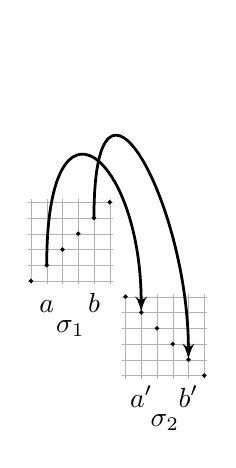
\begin{tikzpicture}
      [
        scale=0.2,
        label/.style={anchor=base}
      ]
      % increasing pattern
      \draw[step=1cm,black!30,ultra thin,fill=black!10] (-0.2,5.8) grid (5.2,11.2);
      \foreach \x/\y in {0/6,1/7,2/8,3/9,4/10,5/11} {
          \draw [fill=black] (\x,\y) circle (0.1);
      }
      % decreasing pattern
      \draw[step=1cm,black!30,ultra thin,fill=black!10] (5.8,-0.2) grid (11.2,5.2);
      \foreach \x/\y in {6/5,7/4,8/3,9/2,10/1,11/0} {
          \draw [fill=black] (\x,\y) circle (0.1);
      }
      % labels
      \node [label] (a) at (1,4) {$a$};
      \node [label] (b) at (4,4) {$b$};
      \node [label] (ap) at (7,-2) {$a'$};
      \node [label] (bp) at (10,-2) {$b'$};
      \node (nu1) at (2.5,3) {$\sigma_1$};
      \node (nu2) at (8.5,-3) {$\sigma_2$};
      % crossings edges
      \draw [line width=1pt,->,>=latex']
      (1,7) .. controls +(0,12) and +(0,10) .. (7,4);
      \draw [line width=1pt,->,>=latex']
      (4,10) .. controls +(0,12) and +(0,10) .. (10,1);
    \end{tikzpicture}
    \;
    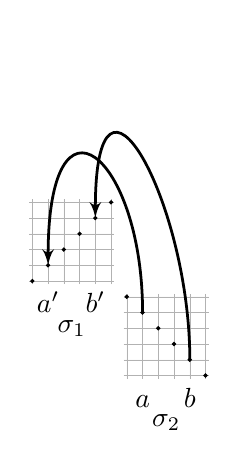
\begin{tikzpicture}
      [
        scale=0.2,
        label/.style={anchor=base}
      ]
      % increasing pattern
      \draw[step=1cm,black!30,ultra thin,fill=black!10] (-0.2,5.8) grid (5.2,11.2);
      \foreach \x/\y in {0/6,1/7,2/8,3/9,4/10,5/11} {
          \draw [fill=black] (\x,\y) circle (0.1);
      }
      % decreasing pattern
      \draw[step=1cm,black!30,ultra thin,fill=black!10] (5.8,-0.2) grid (11.2,5.2);
      \foreach \x/\y in {6/5,7/4,8/3,9/2,10/1,11/0} {
          \draw [fill=black] (\x,\y) circle (0.1);
      }
      % labels
      \node [label] (a) at (1,4) {$a'$};
      \node [label] (b) at (4,4) {$b'$};
      \node [label] (ap) at (7,-2) {$a$};
      \node [label] (bp) at (10,-2) {$b$};
      \node (nu1) at (2.5,3) {$\sigma_1$};
      \node (nu2) at (8.5,-3) {$\sigma_2$};
      % crossings edges
      \draw [line width=1pt,<-,>=latex']
      (1,7) .. controls +(0,12) and +(0,10) .. (7,4);
      \draw [line width=1pt,<-,>=latex']
      (4,10) .. controls +(0,12) and +(0,10) .. (10,1);
    \end{tikzpicture}
    \label{subfig:increasing before and above decreasing}
  }% end subfigure
  \qquad
  \subfigure[%
    A decreasing pattern before and below an increasing pattern.
  ]{%
  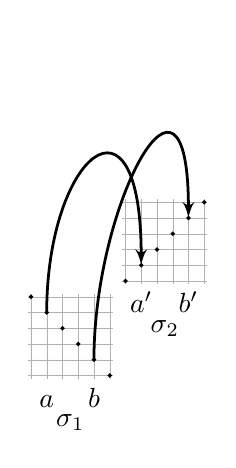
\begin{tikzpicture}
    [
      scale=0.2,
      label/.style={anchor=base}
    ]
    % decreasing pattern
    \draw[step=1cm,black!30,ultra thin,fill=black!10] (-0.2,-0.2) grid (5.2,5.2);
    \foreach \x/\y in {0/5,1/4,2/3,3/2,4/1,5/0} {
        \draw [fill=black] (\x,\y) circle (0.1);
    }
    % decreasing pattern
    \draw[step=1cm,black!30,ultra thin,fill=black!10] (5.8,5.8) grid (11.2,11.2);
    \foreach \x/\y in {6/6,7/7,8/8,9/9,10/10,11/11} {
        \draw [fill=black] (\x,\y) circle (0.1);
    }
    % labels
    \node [label] (a) at (1,-2) {$a$};
    \node [label] (b) at (4,-2) {$b$};
    \node [label] (ap) at (7,4) {$a'$};
    \node [label] (bp) at (10,4) {$b'$};
    \node (nu1) at (2.5,-3) {$\sigma_1$};
    \node (nu2) at (8.5,3) {$\sigma_2$};
    % crossings edges
    \draw [line width=1pt,->,>=latex']
    (1,4) .. controls +(0,10) and +(0,12) .. (7,7);
    \draw [line width=1pt,->,>=latex']
    (4,1) .. controls +(0,10) and +(0,12) .. (10,10);
    \end{tikzpicture}
    \;
    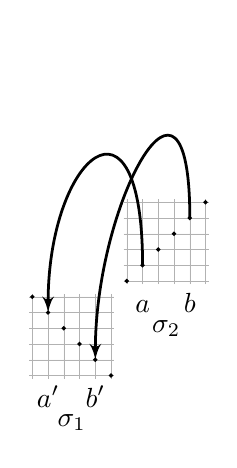
\begin{tikzpicture}
      [
        scale=0.2,
        label/.style={anchor=base}
      ]
      % decreasing pattern
      \draw[step=1cm,black!30,ultra thin,fill=black!10] (-0.2,-0.2) grid (5.2,5.2);
      \foreach \x/\y in {0/5,1/4,2/3,3/2,4/1,5/0} {
          \draw [fill=black] (\x,\y) circle (0.1);
      }
      % decreasing pattern
      \draw[step=1cm,black!30,ultra thin,fill=black!10] (5.8,5.8) grid (11.2,11.2);
      \foreach \x/\y in {6/6,7/7,8/8,9/9,10/10,11/11} {
          \draw [fill=black] (\x,\y) circle (0.1);
      }
      % labels
      \node [label] (a) at (1,-2) {$a'$};
      \node [label] (b) at (4,-2) {$b'$};
      \node [label] (ap) at (7,4) {$a$};
      \node [label] (bp) at (10,4) {$b$};
      \node (nu1) at (2.5,-3) {$\sigma_1$};
      \node (nu2) at (8.5,3) {$\sigma_2$};
      % crossings edges
      \draw [line width=1pt,<-,>=latex']
      (1,4) .. controls +(0,10) and +(0,12) .. (7,7);
      \draw [line width=1pt,<-,>=latex']
      (4,1) .. controls +(0,10) and +(0,12) .. (10,10);
      \end{tikzpicture}
    \label{subfig:decreasing before and below increasing}
  }% end subfigure
  \caption{\label{fig:subfig:no (nu_1, nu_2)-edge}%
    Illustration of Lemma~\ref{lemma:at most one edge monotone}.
  }
\end{figure}

\begin{lemma}
  \label{lemma:at most one edge monotone}
  Let $\pi = \pi_1 \, \sigma_1 \, \pi_2 \, \sigma_2 \, \pi_3$
  be a permutation with $|\sigma_1| \geq 2$ and $|\sigma_2| \geq 2$,
  and $\vv{\mathcal{M}}$ be an oriented perfect matching of $G_\pi$
  that has properties~$\mathbf{P_1}$ and $\mathbf{P_2}$.
  The following assertions hold:
  \begin{enumerate}
    \item
    If $\sigma_1$ is increasing, $\sigma_2$ is decreasing, and
    $\sigma_1$ is above $\sigma_2$
    (see Fig.~\ref{subfig:increasing before and above decreasing}),
    then there is at most one arc between $\sigma_1$ and
    $\sigma_2$ in $\vv{\mathcal{M}}$ (this arc can be a
    $(\sigma_1, \sigma_2)$-arc or a $(\sigma_2, \sigma_1)$-arc).
    \item
    If $\sigma_1$ is decreasing, $\sigma_2$ is increasing, and $\sigma_1$
    is below $\sigma_2$
    (see Fig.~\ref{subfig:decreasing before and below increasing}),
    then there is at most one arc between $\sigma_1$ and
    $\sigma_2$ in $\vv{\mathcal{M}}$ (this arc can be a
    $(\sigma_1, \sigma_2)$-arc or a $(\sigma_2, \sigma_1)$-arc).
  \end{enumerate}
\end{lemma}

\begin{proof}[of Lemma~\ref{lemma:at most one edge monotone}]
  We only prove the first assertion since the proof for the second one
  is similar.
  Suppose, aiming at a contradiction, that the assertion does not hold.
  Therefore, since $\vv{\mathcal{M}}$ has Property~$\mathbf{P_1}$,
  $\vv{\mathcal{M}}$ contains either two crossing $(\sigma_1, \sigma_2)$-arcs
  or two crossing $(\sigma_2, \sigma_1)$-arcs.
  Suppose first that it contains two crossing $(\sigma_1, \sigma_2)$-arcs
  $(a, a')$ and $(b, b')$ with $a < b$.
  Therefore, we have $\pi(a) < \pi(b)$ (since $\sigma_1$ is increasing)
  and $\pi(a') > \pi(b')$ (since
  $\sigma_2$ is decreasing), which contradicts our hypothesis about
  $\vv{\mathcal{M}}$.
  If $\vv{\mathcal{M}}$ contains two crossing $(\sigma_2, \sigma_1)$-arcs
  $(a, a')$ and $(b, b')$ with $a < b$, then
  we have $\pi(a) > \pi(b)$ (since $\sigma_2$ is decreasing)
  and $\pi(a') < \pi(b')$ (since
  $\sigma_2$ is increasing), which contradicts our hypothesis about
  $\vv{\mathcal{M}}$.
  \qed
\end{proof}

\begin{figure}[t!]
  \centering
  \subfigure[%
    $\pi(a) < \pi(a')$.
  ]{%
    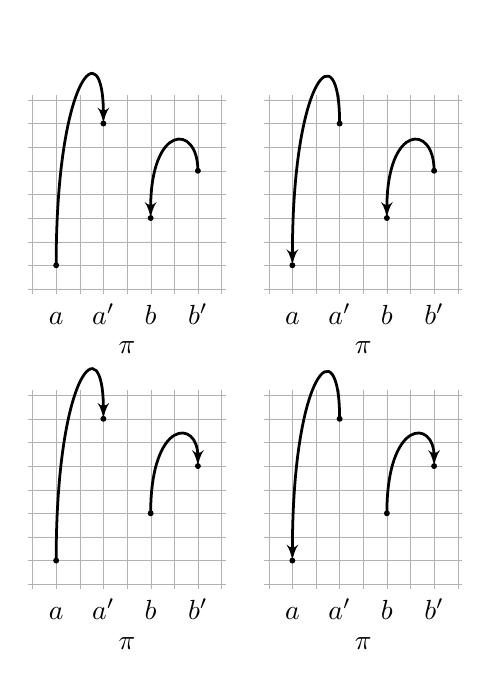
\begin{tikzpicture}
      [
        scale=0.3,
        label/.style={anchor=base}
      ]
      \begin{scope}[]
        % points
        \draw[step=1cm,black!30,ultra thin,fill=black!10] (-0.2,-0.2) grid (8.2,8.2);
        \foreach \x/\y in {1/1,3/7,5/3,7/5} {
            \draw [fill=black] (\x,\y) circle (0.1);
        }
        % labels
        \node [label] (a)  at (1,-1.5)  {$a$};
        \node [label] (ap) at (3,-1.5)  {$a'$};
        \node [label] (b)  at (5,-1.5)  {$b$};
        \node [label] (bp) at (7,-1.5) {$b'$};
        \node (nu1) at (4,-2.5) {$\pi$};
        % arcs
        \draw [line width=1pt,->,>=latex']
        (1,1) .. controls +(0,8) and +(0,4) .. (3,7);
        \draw [line width=1pt,->,>=latex']
        (5,3) .. controls +(0,4) and +(0,2) .. (7,5);
      \end{scope}
      \begin{scope}[yshift=12.5cm]
        % points
        \draw[step=1cm,black!30,ultra thin,fill=black!10] (-0.2,-0.2) grid (8.2,8.2);
        \foreach \x/\y in {1/1,3/7,5/3,7/5} {
            \draw [fill=black] (\x,\y) circle (0.1);
        }
        % labels
        \node [label] (a)  at (1,-1.5)  {$a$};
        \node [label] (ap) at (3,-1.5)  {$a'$};
        \node [label] (b)  at (5,-1.5)  {$b$};
        \node [label] (bp) at (7,-1.5) {$b'$};
        \node (nu1) at (4,-2.5) {$\pi$};
        % arcs
        \draw [line width=1pt,->,>=latex']
        (1,1) .. controls +(0,8) and +(0,4) .. (3,7);
        \draw [line width=1pt,<-,>=latex']
        (5,3) .. controls +(0,4) and +(0,2) .. (7,5);
      \end{scope}
      %
      \begin{scope}[xshift=10cm]
        % points
        \draw[step=1cm,black!30,ultra thin,fill=black!10] (-0.2,-0.2) grid (8.2,8.2);
        \foreach \x/\y in {1/1,3/7,5/3,7/5} {
            \draw [fill=black] (\x,\y) circle (0.1);
        }
        % labels
        \node [label] (a)  at (1,-1.5)  {$a$};
        \node [label] (ap) at (3,-1.5)  {$a'$};
        \node [label] (b)  at (5,-1.5)  {$b$};
        \node [label] (bp) at (7,-1.5) {$b'$};
        \node (nu1) at (4,-2.5) {$\pi$};
        % arcs
        \draw [line width=1pt,<-,>=latex']
        (1,1) .. controls +(0,8) and +(0,4) .. (3,7);
        \draw [line width=1pt,->,>=latex']
        (5,3) .. controls +(0,4) and +(0,2) .. (7,5);
      \end{scope}
    %
      \begin{scope}[xshift=10cm,yshift=12.5cm]
        % points
        \draw[step=1cm,black!30,ultra thin,fill=black!10] (-0.2,-0.2) grid (8.2,8.2);
        \foreach \x/\y in {1/1,3/7,5/3,7/5} {
            \draw [fill=black] (\x,\y) circle (0.1);
        }
        % labels
        \node [label] (a)  at (1,-1.5)  {$a$};
        \node [label] (ap) at (3,-1.5)  {$a'$};
        \node [label] (b)  at (5,-1.5)  {$b$};
        \node [label] (bp) at (7,-1.5) {$b'$};
        \node (nu1) at (4,-2.5) {$\pi$};
        % arcs
        \draw [line width=1pt,<-,>=latex']
        (1,1) .. controls +(0,8) and +(0,4) .. (3,7);
        \draw [line width=1pt,<-,>=latex']
        (5,3) .. controls +(0,4) and +(0,2) .. (7,5);
      \end{scope}
    \end{tikzpicture}
    \label{subfig:decreasing before and below increasing}
  }% end subfigure
  \qquad\;
  \subfigure[%
    $\pi(a) < \pi(a')$.
  ]{%
    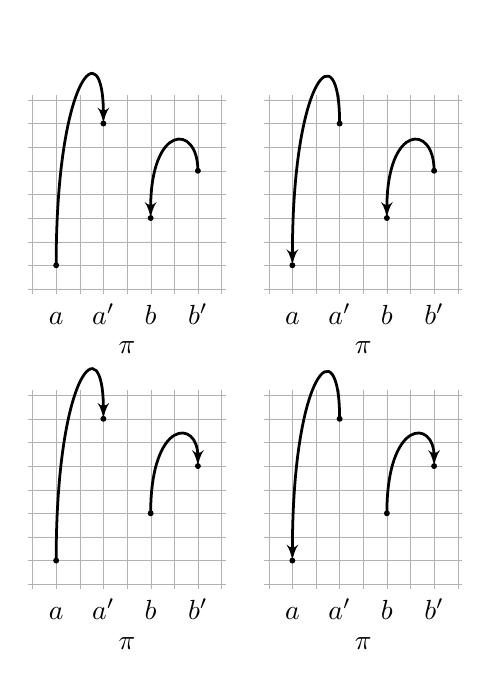
\begin{tikzpicture}
      [
        scale=0.3,
        label/.style={anchor=base}
      ]
      \begin{scope}[]
        % points
        \draw[step=1cm,black!30,ultra thin,fill=black!10] (-0.2,-0.2) grid (8.2,8.2);
        \foreach \x/\y in {1/1,3/7,5/3,7/5} {
            \draw [fill=black] (\x,\y) circle (0.1);
        }
        % labels
        \node [label] (a)  at (1,-1.5)  {$a$};
        \node [label] (ap) at (3,-1.5)  {$a'$};
        \node [label] (b)  at (5,-1.5)  {$b$};
        \node [label] (bp) at (7,-1.5) {$b'$};
        \node (nu1) at (4,-2.5) {$\pi$};
        % arcs
        \draw [line width=1pt,->,>=latex']
        (1,1) .. controls +(0,8) and +(0,4) .. (3,7);
        \draw [line width=1pt,->,>=latex']
        (5,3) .. controls +(0,4) and +(0,2) .. (7,5);
      \end{scope}
      \begin{scope}[yshift=12.5cm]
        % points
        \draw[step=1cm,black!30,ultra thin,fill=black!10] (-0.2,-0.2) grid (8.2,8.2);
        \foreach \x/\y in {1/1,3/7,5/3,7/5} {
            \draw [fill=black] (\x,\y) circle (0.1);
        }
        % labels
        \node [label] (a)  at (1,-1.5)  {$a$};
        \node [label] (ap) at (3,-1.5)  {$a'$};
        \node [label] (b)  at (5,-1.5)  {$b$};
        \node [label] (bp) at (7,-1.5) {$b'$};
        \node (nu1) at (4,-2.5) {$\pi$};
        % arcs
        \draw [line width=1pt,->,>=latex']
        (1,1) .. controls +(0,8) and +(0,4) .. (3,7);
        \draw [line width=1pt,<-,>=latex']
        (5,3) .. controls +(0,4) and +(0,2) .. (7,5);
      \end{scope}
      %
      \begin{scope}[xshift=10cm]
        % points
        \draw[step=1cm,black!30,ultra thin,fill=black!10] (-0.2,-0.2) grid (8.2,8.2);
        \foreach \x/\y in {1/1,3/7,5/3,7/5} {
            \draw [fill=black] (\x,\y) circle (0.1);
        }
        % labels
        \node [label] (a)  at (1,-1.5)  {$a$};
        \node [label] (ap) at (3,-1.5)  {$a'$};
        \node [label] (b)  at (5,-1.5)  {$b$};
        \node [label] (bp) at (7,-1.5) {$b'$};
        \node (nu1) at (4,-2.5) {$\pi$};
        % arcs
        \draw [line width=1pt,<-,>=latex']
        (1,1) .. controls +(0,8) and +(0,4) .. (3,7);
        \draw [line width=1pt,->,>=latex']
        (5,3) .. controls +(0,4) and +(0,2) .. (7,5);
      \end{scope}
    %
      \begin{scope}[xshift=10cm,yshift=12.5cm]
        % points
        \draw[step=1cm,black!30,ultra thin,fill=black!10] (-0.2,-0.2) grid (8.2,8.2);
        \foreach \x/\y in {1/1,3/7,5/3,7/5} {
            \draw [fill=black] (\x,\y) circle (0.1);
        }
        % labels
        \node [label] (a)  at (1,-1.5)  {$a$};
        \node [label] (ap) at (3,-1.5)  {$a'$};
        \node [label] (b)  at (5,-1.5)  {$b$};
        \node [label] (bp) at (7,-1.5) {$b'$};
        \node (nu1) at (4,-2.5) {$\pi$};
        % arcs
        \draw [line width=1pt,<-,>=latex']
        (1,1) .. controls +(0,8) and +(0,4) .. (3,7);
        \draw [line width=1pt,<-,>=latex']
        (5,3) .. controls +(0,4) and +(0,2) .. (7,5);
      \end{scope}
    \end{tikzpicture}
    \label{subfig:decreasing before and below increasing}
  }% end subfigure
  \caption{\label{fig:subfig:value inclusion of arcs}%
    Illustration of Lemma~\ref{lemma:value inclusion of arcs}
    for $\min\{\pi(a), \pi(a')\} < \min\{\pi(b), \pi(b')\}$
    and
    $\max\{\pi(a), \pi(a')\} > \max\{\pi(b), \pi(b')\}$.
  }
\end{figure}

\begin{lemma}
  \label{lemma:value inclusion of arcs}
  Let $\pi$ be a permutation
  and $\vv{\mathcal{M}}$ be an oriented perfect matching of
  the linear graph $G_\pi$.
  If $\vv{\mathcal{M}}$ has Property $\mathbf{P_2}$ then it avoids patterns
  $$
  \LabeledPrecedenceLL{.3}{$a$}{$a'$}{$b$}{$b'$},
  \qquad
  \LabeledPrecedenceLR{.3}{$a$}{$a'$}{$b$}{$b'$},
  \qquad
  \LabeledPrecedenceRL{.3}{$a$}{$a'$}{$b$}{$b'$},
  \qquad
  \LabeledPrecedenceRR{.3}{$a$}{$a'$}{$b$}{$b'$}
  $$
  for
  (i)
  $\min\{\pi(a), \pi(a')\} < \min\{\pi(b), \pi(b')\}$
  and
  $\max\{\pi(a), \pi(a')\} > \max\{\pi(b), \pi(b')\}$
  and
  (ii)
  $\min\{\pi(a), \pi(a')\} > \min\{\pi(b), \pi(b')\}$
  and
  $\max\{\pi(a), \pi(a')\} < \max\{\pi(b), \pi(b')\}$.
\end{lemma}

\begin{proof}[of Lemma~\ref{lemma:value inclusion of arcs}]
  We only prove the lemma for case \emph{(i)}
  since the proof for case \emph{(ii)} is similar.
  Therefore, assume
  $\min\{\pi(a), \pi(a')\} < \min\{\pi(b), \pi(b')\}$
  and
  $\max\{\pi(a), \pi(a')\} > \max\{\pi(b), \pi(b')\}$,
  and suppose, aiming at a contradiction, that the assertion of the lemma
  does not hold.
  We need to consider two cases.
  For each of the following patterns
  $$
  \LabeledPrecedenceLL{.3}{$a$}{$a'$}{$b$}{$b'$},
  \qquad
  \LabeledPrecedenceLR{.3}{$a$}{$a'$}{$b$}{$b'$},
  $$
  we have
  $\pi(a) < \pi(b)$ and $\pi(a') > \pi(b')$,
  and
  for each of the following patterns
  $$
  \LabeledPrecedenceRL{.3}{$a$}{$a'$}{$b$}{$b'$},
  \qquad
  \LabeledPrecedenceRR{.3}{$a$}{$a'$}{$b$}{$b'$},
  $$
  we have
  $\pi(a) > \pi(b)$ and $\pi(a') < \pi(b')$.
  Hence, it follows that $\vv{\mathcal{M}}$ does not have
  Property $\mathbf{P_2}$. This is a contradiction.
  \qed
\end{proof}

\begin{lemma}
  \label{lemma:for nu_1 and nu_2}
  Let $\pi = \pi_1 \, \sigma_1 \, \pi_2 \, \sigma_2 \, \pi_3$
  be a permutation where $\sigma_1$ is an increasing pattern of
  length $k$, $k \geq 3$,  and $\sigma_2$ is below $\sigma_1$,
  and $\vv{\mathcal{M}}$ be an oriented perfect matching of $G_\pi$
  that has properties $\mathbf{P_1}$ and $\mathbf{P_2}$.
  If $\vv{\mathcal{M}}$ contains either a $(\sigma_1, \sigma_2)$-arc
  or a $(\sigma_2, \sigma_1)$-arc,
  then it does not contain a $(\sigma_1, \sigma_1)$-arc.
\end{lemma}

\begin{proof}[of Lemma~\ref{lemma:for nu_1 and nu_2}]
  Suppose first that $\vv{\mathcal{M}}$ contains a $(\sigma_1, \sigma_2)$-arc,
  say $(a, a')$.
  (The proof for the case $\vv{\mathcal{M}}$ contains a
  $(\sigma_2, \sigma_1)$-arc is similar.)
  Now, suppose, aiming at a contradiction, that the assertion does not hold and
  that $\vv{\mathcal{M}}$ contains a $(\sigma_1, \sigma_1)$-arc, say $(b, b')$.
  Since $\vv{\mathcal{M}}$ has Property $\mathbf{P_1}$, it avoids
  \InclusionLL,~\InclusionLR,~\InclusionRL,~\InclusionRR,~\CrossingLR
  and \CrossingRL,
  and hence $(a, a')$ and $(b, b')$ are either crossing arcs
  with $b < a < b'$, or $(b, b')$ precedes $(a, a')$.
  We consider the two cases.
  \begin{itemize}
    \item
    If $(a, a')$ and $(b, b')$ are crossing arcs with $b < a < b'$,
    then we have
    $\pi(b) < \pi(a)$ (since $\sigma_1$ is increasing) and
    $\pi(b') < \pi(a')$ (since $\sigma_1$ is above $\sigma_2$).
    Then it follows that $\vv{\mathcal{M}}$ does not have
    Property $\mathbf{P_2}$. This is a contradiction.
    \item
    If $(b, b')$ precedes $(a, a')$, then we have
    $\min(b,b') > a'$ and $\max(b, b') < a$.
    But $\sigma_1$ is above $\sigma_2$, and hence, according
    to Lemma~\ref{lemma:value inclusion of arcs},
    $\vv{\mathcal{M}}$ does not have
    Property $\mathbf{P_2}$. This is a contradiction.
  \end{itemize}
  \qed
\end{proof}


\begin{lemma}
  \label{lemma:reverse oriented matching}
  Let $\pi$ be a permutation
  and $\vv{\mathcal{M}}$ be an oriented perfect matching of
  the linear graph $G_\pi$.
  If $\vv{\mathcal{M}}$ has properties $\mathbf{P_1}$ and $\mathbf{P_2}$ then
  so does the oriented perfect matching
  $\vv{\mathcal{M}^r}$ obtained from $\vv{\mathcal{M}}$ by reversing
  each arc.
\end{lemma}

\begin{proof}[of Lemma~\ref{lemma:reverse oriented matching}]
  This is immediate for Property~$\mathbf{P_2}$,
  since, for any two arcs $(a, a')$ and $(b,b')$ of $\vv{\mathcal{M}}$,
  we have $\pi(a) < \pi(b)$ if and only if $\pi(a') < \pi(b')$.
  As for Property~$\mathbf{P_1}$, it is enough to observe that
  the set \InclusionLL,~\InclusionLR,~\InclusionRL,~\InclusionRR,~\CrossingLR
  or \CrossingRL is closed by arc reversals
  \qed
\end{proof}

A direct interpretation of Lemma~\ref{lemma:reverse oriented matching} is that,
if a permutation $\pi$ is a square, one can exchange the roles of the two
order-isomorphic patterns that cover $\pi$.
An immediate but useful consequence of Lemma~\ref{lemma:reverse oriented matching}
reads as follows.

\begin{corollary}
  \label{corollary:reverse oriented matching}
  Let $\pi$ be a permutation and $a$ and $a'$ be two vertices of
  the linear graph $G_\pi$.
  There exists an oriented perfect matching of $G_\pi$ with
  properties $\mathbf{P_1}$ and $\mathbf{P_2}$ that contains arc $(a,a')$
  if and only of
  there exists an oriented perfect matching of $G_\pi$ with
  properties $\mathbf{P_1}$ and $\mathbf{P_2}$ that contains arc $(a',a)$
\end{corollary}

Having disposed of these preliminary observations,
we now turn to proving hardness of the targeted problem.

\begin{proposition}
  \label{proposition:hardness}
  Deciding whether a permutation is a square is \NPC.
\end{proposition}

\begin{proof}[of Proposition~\ref{proposition:hardness}]
  The problem is certainly in $\NPclass$. We propose a reduction from
  the pattern involvement problem which is known to be
  \NPC~\cite{Bose:Buss:Lubiw:1998}. Given two permutations $\pi$ and
  $\sigma$, pattern involvement problem is to decide whether $\sigma$ occurs in
  $\pi$ (as an order-isomorphic pattern).

  \begin{figure}[t!]
    \centering
    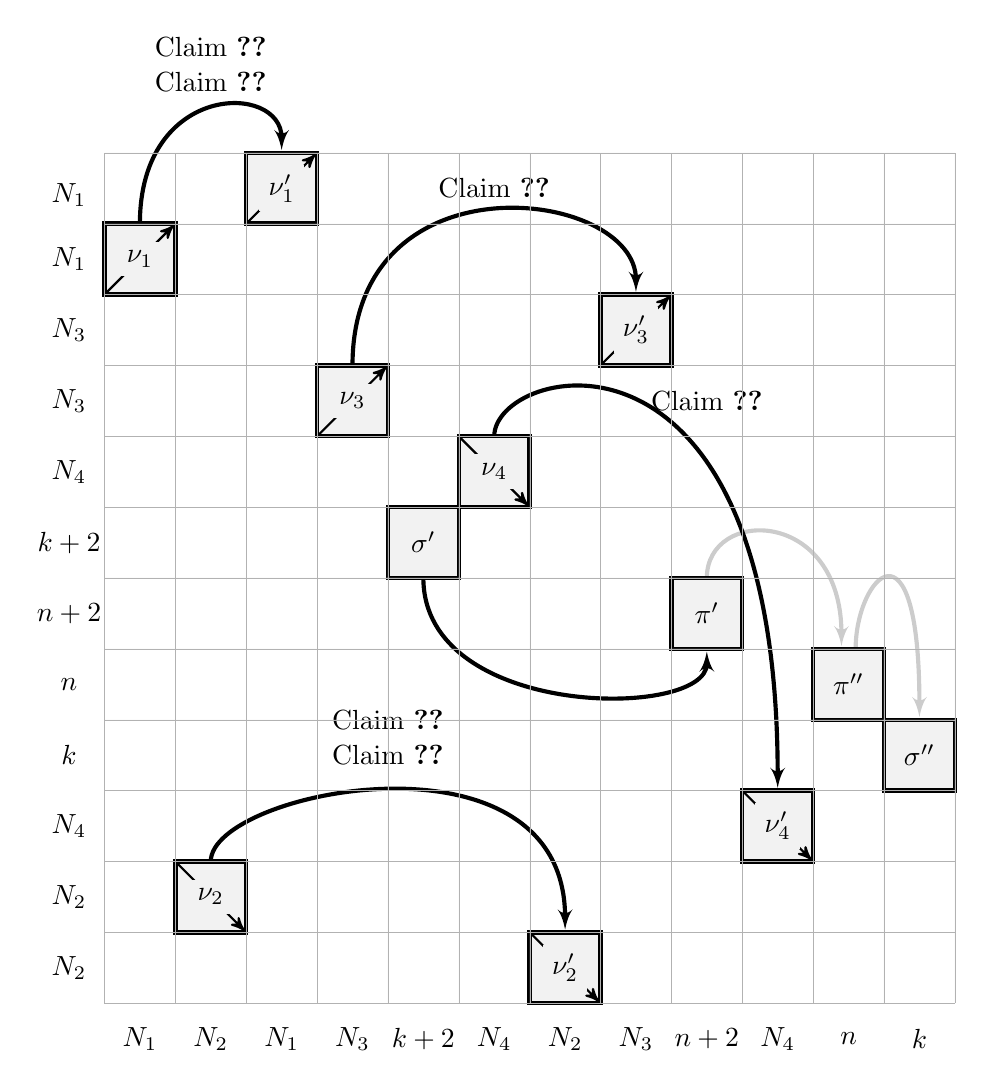
\begin{tikzpicture}[
      scale=.9,
      >=stealth',
      shorten >=1pt,
      main node/.style={align=center},
      cell/.style={draw,ultra thick,fill=black!5},
      structure link/.style={line width=1.5pt},
      pattern link/.style={line width=1.5pt,black!20},
      monotone/.style={->,thick}
      ]
      % arcs
      % pi 1 - pi 2
      \draw [pattern link,->,>=latex'] (8.5,6) .. controls +(0,1) and +(0,2) .. (10.4,5);
      % pi 2 - sigma 2
      \draw [pattern link,->,>=latex'] (10.6,5) .. controls +(0,1) and +(0,3) .. (11.5,4);
      % 1
      \draw [structure link,->,>=latex'] (0.5,11) .. controls +(0,2) and +(0,1) .. (2.5,12);
      \node (claim edge 1) at (1.5,13.5) {Claim~\ref{claim:(nu_1, nu'_1)-edge}};
      \node (claim edge 1) at (1.5,13) {Claim~\ref{claim:all (nu_1, nu'_1)-edges}};
      % 2
      \draw [structure link,->,>=latex'] (1.5,2) .. controls +(0,1) and +(0,3) .. (6.5,1);
      \node (claim edge 2) at (4,4) {Claim~\ref{claim:(nu_2, nu'_2)-edge}};
      \node (claim edge 2) at (4,3.5) {Claim~\ref{claim:all (nu_2, nu'_2)-edges}};
      % 3
      \draw [structure link,->,>=latex'] (3.5,9) .. controls +(0,3) and +(0,1.5) .. (7.5,10);
      \node (claim edge 1) at (5.5,11.5) {Claim~\ref{claim:(nu_3, nu'_3)-edge}};
      % 4
      \draw [structure link,->,>=latex'] (5.5,8) .. controls +(0,1) and +(0,7) .. (9.5,3);
      \node (claim edge 1) at (8.5,8.5) {Claim~\ref{claim:(nu_4, nu'_4)-edge}};
      % sigma 1 - pi 1
      \draw [structure link,->,>=latex'] (4.5,6) .. controls +(0,-2) and +(0,-1) .. (8.5,5);
      % \node (claim edge 1) at (6.5,4) {Claim~\ref{}};
      % nodes
      % 1
      \draw [cell] (0,10) -- (1,10) -- (1,11) -- (0,11) -- cycle;
      \draw [monotone] (0,10) -- ++(1,1) node [midway,fill=white,fill=black!5] {$\nu_1$};
      %\draw [draw,ultra thick,fill=black!5] (0,10) -- (1,10) -- (1,11) -- (0,11) -- cycle;
      \draw [cell] (2,11) -- (3,11) -- (3,12) -- (2,12) -- cycle;
      \draw [monotone] (2,11) -- ++(1,1) node [midway,fill=white,fill=black!5] {$\nu'_1$};
      % 2
      \draw [cell] (1,1) -- (2,1) -- (2,2) -- (1,2) -- cycle;
      \draw [monotone] (1,2) -- ++(1,-1) node [midway,fill=white,fill=black!5] {$\nu_2$};
      \draw [cell] (6,0) -- (7,0) -- (7,1) -- (6,1) -- cycle;
      \draw [monotone] (6,1) -- ++(1,-1) node [midway,fill=white,fill=black!5] {$\nu'_2$};
      % 3
      \draw [cell] (3,8) -- (4,8) -- (4,9) -- (3,9) -- cycle;
      \draw [monotone] (3,8) -- ++(1,1) node [midway,fill=white,fill=black!5] {$\nu_3$};
      \draw [cell] (7,9) -- (8,9) -- (8,10) -- (7,10) -- cycle;
      \draw [monotone] (7,9) -- ++(1,1) node [midway,fill=white,fill=black!5] {$\nu'_3$};
      % 4
      \draw [cell] (5,7) -- (6,7) -- (6,8) -- (5,8) -- cycle;
      \draw [monotone] (5,8) -- ++(1,-1) node [midway,fill=white,fill=black!5] {$\nu_4$};
      \draw [cell] (9,2) -- (10,2) -- (10,3) -- (9,3) -- cycle;
      \draw [monotone] (9,3) -- ++(1,-1) node [midway,fill=white,fill=black!5] {$\nu'_4$};
      % sigma 1
      \draw [cell] (4,6) -- (5,6) -- (5,7) -- (4,7) -- cycle;
      \node [main node] (sigma1) at (4.5,6.5) {$\sigma'$};
      % pi 1
      \draw [cell] (8,5) -- (9,5) -- (9,6) -- (8,6) -- cycle;
      \node [main node] (pi1) at (8.5,5.5) {$\pi'$};
      % pi 2
      \draw [cell] (10,4) -- (11,4) -- (11,5) -- (10,5) -- cycle;
      \node [main node] (sigma2) at (10.5,4.5) {$\pi''$};
      % sigma 2
      \draw [cell] (11,3) -- (12,3) -- (12,4) -- (11,4) -- cycle;
      \node [main node] (pi2) at (11.5,3.5) {$\sigma''$};
      % grid
      \draw[step=1cm,black!30,ultra thin,fill=black!10] (0,0) grid (12,12);
      % row size
      \foreach \y/\N in {0.5/N_2,1.5/N_2,2.5/N_4,3.5/k,4.5/n,5.5/n+2,6.5/k+2,7.5/N_4,8.5/N_3,9.5/N_3,10.5/N_1,11.4/N_1} {
          \node at (-0.5,\y) (R\y) {$\N$};
      }
      % column size
      \foreach \x/\N in
      {0.5/N_1,1.5/N_2,2.5/N_1,3.5/N_3,4.5/k+2,5.5/N_4,6.5/N_2,7.5/N_3,8.5/n+2,9.5/N_4,10.5/n,11.5/k} {
          \node at (\x,-0.5) (C\x) {$\N$};
      }
    \end{tikzpicture}
    \caption{\label{fig:reduction}%
      Schematic representation of the permutation $\mu$ used
      in Proposition~\ref{proposition:hardness}.
      Black arcs denote the presence of at least one arc between two bunches of
      positions in $\mu$.
      Grey arcs denote edges that are only considered in the forward direction of the
      proof.
    }%
  \end{figure}

  Let $\pi \in S_n$ and $\sigma \in S_k$ be two arbitrary permutations.
  Define
  \begin{align*}
  N_4 &= 2(2n + k + 2) + 1  = 4n + 2k + 5 \\
  N_3 &= 2(2N_4 + 2n + 2k + 4) + 1 = 20n + 12k + 9 \\
  N_2 &= 2(2N_3 + 2N_4 + 2n + 2k + 4) + 1 \\
  N_1 &= 2(2N_2 + 2N_3 + 2N_4 + 2n + 2k + 4) + 1\text{.}
  \end{align*}
  Notice that $N_1, N_2, N_3$ and $N_4$ are polynomial in $n$.
  The crucial properties are that
  (i) $N_1, N_2, N_3$ and $N_4$ are odd integers
  and
  (ii) $N_i > \left(\sum_{i < j \leq 4} 2N_j\right) + 2n + 2k + k$
  for every $1 \leq i \leq 4$.

  We now turn to defining various gadgets (sequences of integers)
  that act as building blocks in our construction of a new permutation $\mu$:
  \begin{align*}
  \sigma'  &= ((k+1) \; \sigma \; (k+2)) \; [2N_2 + N_4 + 2n + k + 2] \\
  \pi'     &= ((n+1) \; \pi \; (n+2)) \; [2N_2 + N_4 + n + k + 2] \\
  \sigma'' &= \sigma \; [2N_2 + N_4] \\
  \pi''    &= \pi \; [2N_2 + N_4 + k] \\
  \nu_1    &= \nearrow_{N_1} \; [2N_2 + 2N_3 + 2N_4 + 2n + 2k + 4] \\
  \nu'_1   &= \nearrow_{N_1} \; [N_1 + 2N_2 + 2N_3 + 2N_4 + 2n + 2k + 4] \\
  \nu_2    &= \nearrow_{N_2} \; [N_2] \\
  \nu'_2   &= \searrow_{N_2} \\
  \nu_3    &= \nearrow_{N_3} \; [2N_2 + 2N_4 + 2n + 2k + 4] \\
  \nu'_3   &= \nearrow_{N_3} \; [2N_2 + N_3 + 2N_4 + 2n + 2k + 4] \\
  \nu_4    &= \searrow_{N_4} \; [2N_2 + N_4 + 2n + 2k + 4] \\
  \nu'_4   &= \searrow_{N_4} \; [2N_2]\text{.}
  \end{align*}
  We are now in position to define our target permutation $\mu$
  (see Fig.~\ref{fig:reduction} for an illustration):
  $$
  \mu
  =
  \nu_1 \; \nu_2 \; \nu'_1 \; \nu_3 \; \sigma' \; \nu_4 \; \nu'_2 \; \nu'_3 \; \pi' \; \nu'_4 \; \pi'' \; \sigma''
  \text{.}
  $$

  It is immediate that H can be constructed in polynomial-time in $n$ and $k$.
  We claim that $\sigma$ occurs in $\pi$ if and only if
  there exists an oriented perfect matching
  $\vv{\mathcal{M}}$ of $G_\mu$ that has properties $\mathbf{P_1}$ and
  $\mathbf{P_2}$.

  Suppose first that $\sigma$ occurs in $\pi$ and fix an occurrence.
  Construct an oriented matching $\vv{\mathcal{M}}$ as follows
  (all arcs are oriented to the left):
  \begin{itemize}
    \item $\mathcal{M}$ contains $N_1$ pairwise crossing
    $(\nu_1, \nu'_1)$-arcs.
    \item $\mathcal{M}$ contains $N_2$ pairwise crossing
    $(\nu_2, \nu'_2)$-arcs.
    \item $\mathcal{M}$ contains $N_3$ pairwise crossing
    $(\nu_3, \nu'_3)$-arcs.
    \item $\mathcal{M}$ contains $N_4$ pairwise crossing
    $(\nu_4, \nu'_4)$-arcs.
    \item $\mathcal{M}$ contains $k+2$ pairwise crossing
    $(\sigma', \pi')$-arcs as depicted in
    Figure~\ref{fig:subfig:sigma' - pi' - pi'' - sigma''}.
    More precisely,
    (i) the first position of $\sigma'$
    (\emph{i.e.}, $(2N_1+N_2+N_3) + 1$) is linked
    to the first position of $\pi'$
    (\emph{i.e.}, $(2N_1 + 2N_2 + 2N_3 + N_4 + k + 2) + 1$),
    (ii) the last position of $\sigma'$
    (\emph{i.e.}, $(2N_1+N_2+N_3) + k+2$) is linked
    to the last position of $\pi'$
    (\emph{i.e.}, $(2N_1 + 2N_2 + 2N_3 + N_4 + k + 2) + n+2$),
    and all other positions in $\sigma'$ are linked by means of $k$ pairwise
    crossing arcs to the positions in
    $\pi'$ that correspond to the fixed occurence of $\sigma$ in $\pi$.
    (Notice that we use here the fact that $\sigma$ occurs in $\pi$).
    \item $\mathcal{M}$ contains $n-k$ pairwise crossing
    $(\pi', \pi'')$-arcs as depicted in
    Figure~\ref{fig:subfig:sigma' - pi' - pi'' - sigma''}.
    More precisely,
    all positions in $\pi'$ that do not correspond to the fixed occurence of
    $\sigma$ in $\pi$ are linked by means of $n-k$ pairwise crossing arcs
    to the positions in $\pi''$ that do not correspond to the fixed
    occurrence of $\sigma$ in $\pi$.
    \item $\mathcal{M}$ contains $k$ pairwise crossing
    $(\pi'', \sigma'')$-arcs as depicted in
    Figure~\ref{fig:subfig:sigma' - pi' - pi'' - sigma''}.
    More precisely, the positions in $\pi''$ that correspond to
    the fixed occurrence of $\sigma$ in $\pi$ are llinked
    linked by means of $k$ pairwise crossing arcs to all positions in
    $\sigma''$.
    (Notice that, again, we use here the fact that $\sigma$ occurs in $\pi$).
  \end{itemize}
  It can be easily checked (probably referring to Figure~\ref{fig:reduction}) that
  $\vv{\mathcal{M}}$ is perfect and has
  properties $\mathbf{P_1}$ and $\mathbf{P_2}$.

    \begin{figure}[t!]
      \centering
        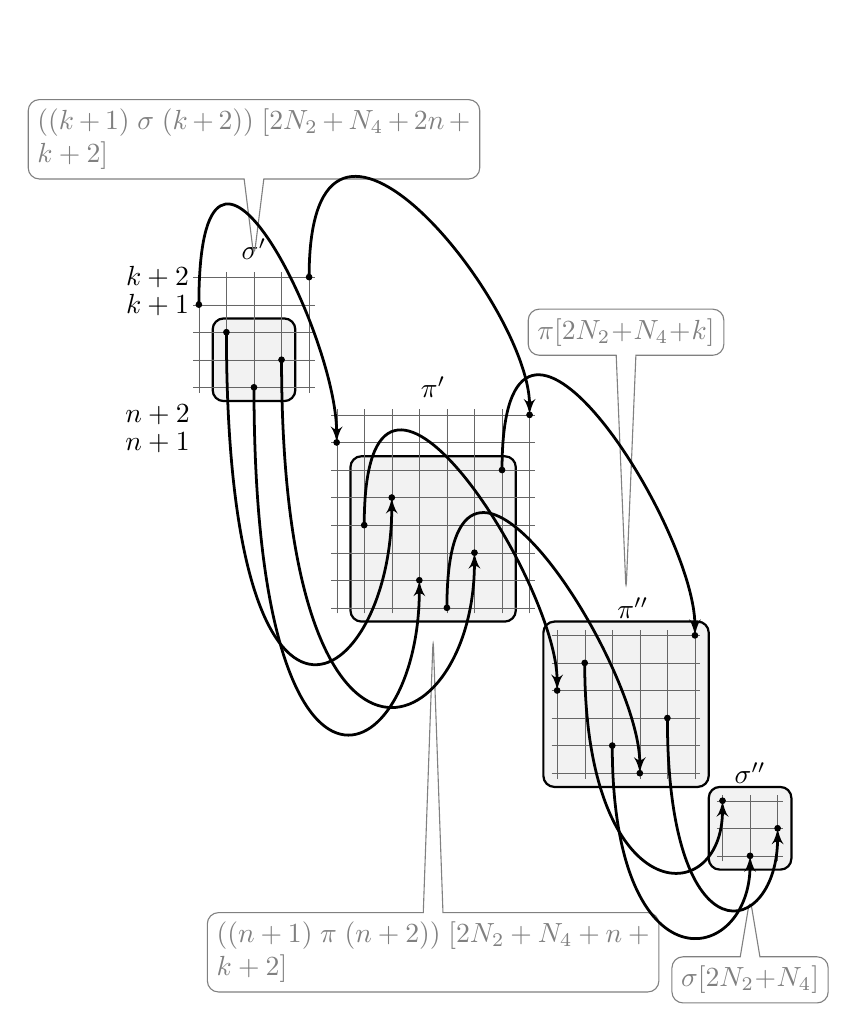
\begin{tikzpicture}
          [
            scale=0.35,
            label/.style={anchor=base},
            cell/.style={draw,thick,fill=black!5}
          ]
          % sigma'
          \draw [cell,rounded corners] (1.5,16.5) -- (4.5,16.5) -- (4.5,19.5) -- (1.5,19.5) -- cycle;
          \draw[step=1cm,black!60,ultra thin,fill=black!10] (0.8,16.8) grid (5.2,21.2);
          \foreach \x/\y in {1/20,2/19,3/17,4/18,5/21} {
              \draw [fill=black] (\x,\y) circle (0.1);
          }
          \node (pip) at (3,22) {$\sigma'$};
          \node[%
            draw,
            text width=5.5cm,text justified,color=black!50,rounded corners,
            rectangle callout,callout relative pointer={(0.0cm,-1cm)}
          ] at (3,26)
          {%
            $((k+1) \; \sigma \; (k+2)) \; [2N_2 + N_4 + 2n + k + 2]$
          };%
          %\node at (3,-0.5) {$((k+1) \; \sigma \; (k+2)) \; [2N_2 + N_4 + 2n + k + 2]$};
          \node at (-0.5,20) {$k+1$};
          \node at (-0.5,21) {$k+2$};
          % pi'
          \draw [cell,rounded corners] (6.5,8.5) -- (12.5,8.5) -- (12.5,14.5) -- (6.5,14.5) -- cycle;
          \draw[step=1cm,black!60,ultra thin,fill=black!10] (5.8,8.8) grid (13.2,16.2);
          \foreach \x/\y in {6/15,7/12,8/13,9/10,10/9,11/11,12/14,13/16} {
              \draw [fill=black] (\x,\y) circle (0.1);
          }
          \node (pip) at (9.5,17) {$\pi'$};
          \node[%
            draw,
            text width=5.5cm,text justified,color=black!50,rounded corners,
            rectangle callout,callout relative pointer={(0.0cm,3.5cm)}
          ] at (9.5,-3.5)
          {%
            $((n+1) \; \pi \; (n+2)) \; [2N_2 + N_4 + n + k + 2]$
          };%
          %\node at (9.5,-2) {$((n+1) \; \pi \; (n+2)) \; [2N_2 + N_4 + n + k + 2]$};
          \node at (-0.5,15) {$n+1$};
          \node at (-0.5,16) {$n+2$};
          % pi''
          \draw [cell,rounded corners] (13.5,2.5) -- (19.5,2.5) -- (19.5,8.5) -- (13.5,8.5) -- cycle;
          \draw[step=1cm,black!60,ultra thin,fill=black!10] (13.8,2.8) grid (19.2,8.2);
          \foreach \x/\y in {14/6,15/7,16/4,17/3,18/5,19/8} {
              \draw [fill=black] (\x,\y) circle (0.1);
          }
          \node (pipp) at (16.75,9) {$\pi''$};
          \node[%
            draw,
            text width=2.25cm,text justified,color=black!50,rounded corners,
            rectangle callout,callout relative pointer={(0.0cm,-3cm)}
          ] at (16.5,19)
          {%
            $\pi [2N_2 + N_4 + k]$
          };%
          %\node at (16.5,-3.5) {$\pi [2N_2 + N_4 + k]$};
          % sigma''
          \draw [cell,rounded corners] (19.5,-0.5) -- (22.5,-.5) -- (22.5,2.5) -- (19.5,2.5) -- cycle;
          \draw[step=1cm,black!60,ultra thin,fill=black!10] (19.8,-0.2) grid (22.2,2.2);
          \foreach \x/\y in {20/2,21/0,22/1} {
              \draw [fill=black] (\x,\y) circle (0.1);
          }
          \node (sigmapp) at (21,3) {$\sigma''$};
          \node[%
            draw,
            text width=1.75cm,text justified,color=black!50,rounded corners,
            rectangle callout,callout relative pointer={(0.0cm,0.75cm)}
          ] at (21,-4.5)
          {%
            $\sigma [2N_2 + N_4]$
          };%
          %\node at (21,-5) {$\sigma [2N_2 + N_4]$};
          % edges sigma' - pi'
          \draw [line width=1pt,->,>=latex']
          (1,20) .. controls +(0,9) and +(0,4) .. (6,15);
          \draw [line width=1pt,->,>=latex']
          (5,21) .. controls +(0,9) and +(0,4) .. (13,16);
          \draw [line width=1pt,->,>=latex']
          (2,19) .. controls +(0,-17) and +(0,-7) .. (8,13);
          \draw [line width=1pt,->,>=latex']
          (3,17) .. controls +(0,-17) and +(0,-7) .. (9,10);
          \draw [line width=1pt,->,>=latex']
          (4,18) .. controls +(0,-17) and +(0,-7) .. (11,11);
          % edges pi' - pi''
          \draw [line width=1pt,->,>=latex']
          (7,12) .. controls +(0,9) and +(0,4) .. (14,6);
          \draw [line width=1pt,->,>=latex']
          (10,9) .. controls +(0,9) and +(0,4) .. (17,3);
          \draw [line width=1pt,->,>=latex']
          (12,14) .. controls +(0,9) and +(0,4) .. (19,8);
          % edges pi'' - sigma''
          \draw [line width=1pt,->,>=latex']
          (15,7) .. controls +(0,-9) and +(0,-4) .. (20,2);
          \draw [line width=1pt,->,>=latex']
          (16,4) .. controls +(0,-9) and +(0,-4) .. (21,0);
          \draw [line width=1pt,->,>=latex']
          (18,5) .. controls +(0,-9) and +(0,-4) .. (22,1);
        \end{tikzpicture}
        \caption{\label{fig:subfig:sigma' - pi' - pi'' - sigma''}%
        Illustration of the containment-free perfect matching $\mathcal{M}$
        between gadgets $\sigma'$, $\pi'$, $\pi''$ and $\sigma''$ assuming two
        input permutation $\sigma = 312$ and $\pi = 4\mathbf{5}\mathbf{2}1\mathbf{3}6$
        (where a specific occurrence of $\sigma$ in $\pi$ is depicted in bold).
        }
      \end{figure}

  Conversely, suppose that there exists an oriented perfect matching
  $\vv{\mathcal{M}}$ in $G_\mu$ that has
  properties $\mathbf{P_1}$ and $\mathbf{P_2}$.
  We show that $\sigma$ occurs as a pattern in $\pi$.
  Whereas the oriented matching $\vv{\mathcal{M}}$ may not be as regular as in the
  forward direction, the main idea is to prove that $\vv{\mathcal{M}}$ contains enough
  structure
  (more precisely, $k+2$ $(\sigma', \pi')$-arcs) so that we can conclude
  that $\sigma$ occurs in $\pi$.
  We have divided the reverse direction into a serie of basic claims that
  progressively defines (and refines)
  the overall structure of $\vv{\mathcal{M}}$.

    \begin{figure}[t!]
      \centering
      \subfigure[%
        A $(\nu_1, \nu_2)$-edge $(a, b)$ together with a
        $(\nu_2, \nu'_1)$-edge $(x, y)$.
        Notice that we may have $x<b$
        (as long as $N_1 < x \leq N_1+N_2$ and $N_1 < b \leq N_1+N_2$
        do hold).
      ]{%
        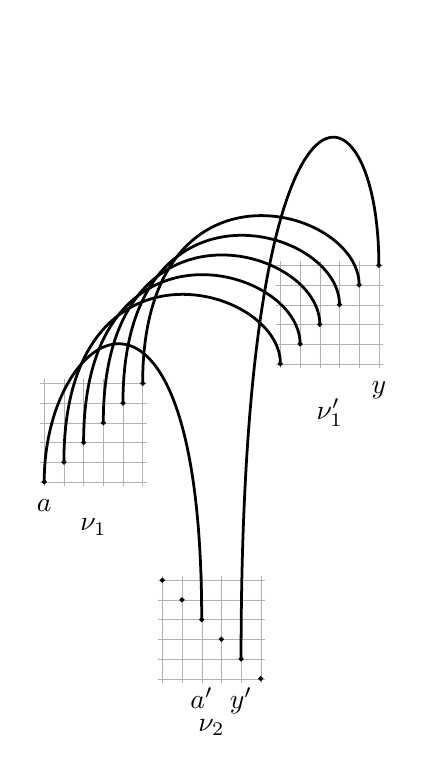
\begin{tikzpicture}
          [
            scale=0.25,
            label/.style={anchor=base}
          ]
          % nu_1
          \draw[step=1cm,black!30,ultra thin,fill=black!10] (-0.2,9.8) grid (5.2,15.2);
          \foreach \x/\y in {0/10,1/11,2/12,3/13,4/14,5/15} {
              \draw [fill=black] (\x,\y) circle (0.1);
          }
          % nu_4
          \draw[step=1cm,black!30,ultra thin,fill=black!10] (5.8,-0.2) grid (11.2,5.2);
          \foreach \x/\y in {6/5,7/4,8/3,9/2,10/1,11/0} {
              \draw [fill=black] (\x,\y) circle (0.1);
          }
          % nu'_1
          \draw[step=1cm,black!30,ultra thin,fill=black!10] (11.8,15.8) grid (17.2,21.2);
          \foreach \x/\y in {12/16,13/17,14/18,15/19,16/20,17/21} {
              \draw [fill=black] (\x,\y) circle (0.1);
          }
          % labels
          \node [label] (y) at (17,14.5) {$y$};
          \node [label] (yp) at (10,-1.5) {$y'$};
          \node [label] (a) at (0,8.5) {$a$};
          \node [label] (ap) at (8,-1.5) {$a'$};
          \node (nu1) at (2.5,7.7) {$\nu_1$};
          \node (nu2) at (8.5,-2.5) {$\nu_2$};
          \node (nu1') at (14.5,13.5) {$\nu'_1$};
          % crossings edges
          \draw [line width=1pt]
          (1,11) .. controls +(0,12) and +(0,4) .. (12,16);
          \draw [line width=1pt]
          (2,12) .. controls +(0,12) and +(0,4) .. (13,17);
          \draw [line width=1pt]
          (3,13) .. controls +(0,12) and +(0,4) .. (14,18);
          \draw [line width=1pt]
          (4,14) .. controls +(0,12) and +(0,4) .. (15,19);
          \draw [line width=1pt]
          (5,15) .. controls +(0,12) and +(0,4) .. (16,20);
          % data edges
          \draw [line width=1pt]
          (0,10) .. controls +(0,8) and +(0,20) .. (8,3);
          \draw [line width=1pt]
          (10,1) .. controls +(0,32) and +(0,10) .. (17,21);
        \end{tikzpicture}
        \label{subfig:no (nu_1, nu_2)-edge - 1}
      }% end subfigure
      \qquad
      \subfigure[%
        A $(\nu_1, \nu'_1)$-edge $(x', y')$ together with an
        edge $(y, z)$ which is neither
        a $(\nu_1, \nu'_1)$-edge,
        nor a $(\nu_2, \nu'_1)$-edge,
        nor a $(\nu'_1, \nu'_1)$-edge.
        Notice that $y$ may be any position satisfying
        $N_1+N_2 < y \leq 2N_1+N_2$.
      ]{%
      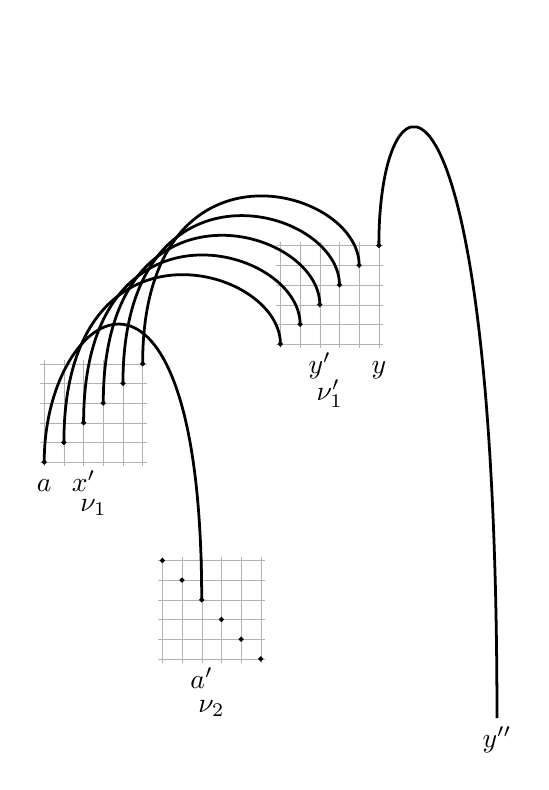
\begin{tikzpicture}
        [
          scale=0.25,
          label/.style={anchor=base}
        ]
        % nu_1
        \draw[step=1cm,black!30,ultra thin,fill=black!10] (-0.2,9.8) grid (5.2,15.2);
        \foreach \x/\y in {0/10,1/11,2/12,3/13,4/14,5/15} {
            \draw [fill=black] (\x,\y) circle (0.1);
        }
        % nu_4
        \draw[step=1cm,black!30,ultra thin,fill=black!10] (5.8,-0.2) grid (11.2,5.2);
        \foreach \x/\y in {6/5,7/4,8/3,9/2,10/1,11/0} {
            \draw [fill=black] (\x,\y) circle (0.1);
        }
        % nu'_1
        \draw[step=1cm,black!30,ultra thin,fill=black!10] (11.8,15.8) grid (17.2,21.2);
        \foreach \x/\y in {12/16,13/17,14/18,15/19,16/20,17/21} {
            \draw [fill=black] (\x,\y) circle (0.1);
        }
        % labels
        \node [label] (y) at (17,14.5) {$y$};
        \node [label] (ypp) at (23,-4.5) {$y''$};
        \node [label] (a) at (0,8.5) {$a$};
        \node [label] (a) at (2,8.5) {$x'$};
        \node [label] (a) at (14,14.5) {$y'$};
        \node [label] (ap) at (8,-1.5) {$a'$};
        \node (nu1) at (2.5,7.7) {$\nu_1$};
        \node (nu2) at (8.5,-2.5) {$\nu_2$};
        \node (nu1') at (14.5,13.5) {$\nu'_1$};
        % crossings edges
        \draw [line width=1pt]
        (1,11) .. controls +(0,12) and +(0,4) .. (12,16);
        \draw [line width=1pt]
        (2,12) .. controls +(0,12) and +(0,4) .. (13,17);
        \draw [line width=1pt]
        (3,13) .. controls +(0,12) and +(0,4) .. (14,18);
        \draw [line width=1pt]
        (4,14) .. controls +(0,12) and +(0,4) .. (15,19);
        \draw [line width=1pt]
        (5,15) .. controls +(0,12) and +(0,4) .. (16,20);
        % data edges
        \draw [line width=1pt]
        (0,10) .. controls +(0,8) and +(0,20) .. (8,3);
        \draw [line width=1pt]
        (17,21) .. controls +(0,10) and +(0,35) .. (23,-3);
        \end{tikzpicture}
        \label{subfig:no (nu_1, nu_2)-edge - 2}
      }% end subfigure
      \caption{\label{fig:subfig:no (nu_1, nu_2)-edge}%
        Claim~\ref{claim:no (nu_1, nu_2)-edge}:
        Assuming a $(\nu_1,\nu_2)$-edge $(a, b)$ in $\mathcal{M}$.
      }
    \end{figure}

  \begin{claim}
    \label{claim:no (nu_1, nu_2)-edge}
    There is no $(\nu_1, \nu_2)$-arc nor $(\nu_2, \nu_1)$-arc in
    $\vv{\mathcal{M}}$.
  \end{claim}

  \begin{proof}[of Claim~\ref{claim:no (nu_1, nu_2)-edge}]
    First, according to Lemma~\ref{lemma:at most one edge monotone},
    there exists at most one arc between $\nu_1$ and $\nu_2$ in $\vv{\mathcal{M}}$
    (regardless of the orientation).
    Suppose now, aiming at a contradiction, that there exists
    exactly one arc between $\nu_1$ and $\nu_2$ in $\vv{\mathcal{M}}$.
    According to Corollary~\ref{corollary:reverse oriented matching}, there is no
    loss of generality in assuming that this is a
    $(\nu_1, \nu_2)$-arc and denote it by $(a, a')$.
    Furtheremore, according to Lemma~\ref{lemma:for nu_1 and nu_2},
    there is no $(\nu_1, \nu_1)$-arc in $\vv{\mathcal{M}}$.
    Now, since $\nu_1$ is increasing and there exists
    exactly one $(\nu_1, \nu_2)$ in $\vv{\mathcal{M}}$,
    we conclude that
    $\vv{\mathcal{M}}$ contains $N_1-1$ pairwise crossing
    $(\nu_1, \nu'_1)$-arcs
    (this follows from the fact that $\vv{\mathcal{M}}$ does not contain \CrossingLR
    nor \CrossingRL).
    But $|\nu_1| = |\nu'_1| = N_1$ and $\vv{\mathcal{M}}$ is perfect,
    and hence there exists a position, say $y$, in $\nu'_1$ that is
    not involved in a $(\nu_1, \nu'_1)$-arc in $\vv{\mathcal{M}}$.
    We rule out this configuration by considering two cases:
    \begin{itemize}
      \item Position $y$ is involved in a $(\nu_2, \nu'_1)$-arc,
      say $(y', y)$.
      Then, we have $\mu(a) > \mu(y')$ (since $\nu_1$ is above $\nu_2$)
      and $\mu(a') < \mu(y)$ (since $\nu_2$ is below $\nu'_1$),
      which contradicts Property~$\mathbf{P_2}$.
      See Fig.~\ref{subfig:no (nu_1, nu_2)-edge - 1}.
      \item
      Position $y$ is involved in a $(\nu'_1, \nu_2)$-edge,
      say $(y', y)$.
      According to Lemma~\ref{lemma:value inclusion of arcs},
      $(a, a')$ and $(y, y')$ must be crossing
      (\emph{i.e.}, $y < a'$).
      But it follows that $\vv{\mathcal{M}}$ contains \CrossingLR
      which contradicts Property~$\mathbf{P_1}$.
      \item
      $(y, y'')$ in an arc of $\vv{\mathcal{M}}$ for some
      $y'' > 2N_1 + N_2$.
      But $\nu'_1$ is above any other gadget, and hence
      applying Lemma~\ref{lemma:value inclusion of arcs} to
      arcs
      $(a, a')$ and $(y, y'')$ yields a contrdiction.
      See Fig.~\ref{subfig:no (nu_1, nu_2)-edge - 2}.
    \end{itemize}
    \qed
  \end{proof}

  \begin{claim}
    \label{claim:(nu_1, nu'_1)-edge}
    There is at least one $(\nu_1, \nu'_1)$-arc in $\vv{\mathcal{M}}$.
  \end{claim}

  \begin{proof}[of Claim~\ref{claim:(nu_1, nu'_1)-edge}]
    Suppose, aiming at a contradiction, that there is no arc between
    $\nu_1$ and $\nu'_1$ in $\vv{\mathcal{M}}$.
    Then it follows that there exists an arc $(x, x')$ or
    $(x', x)$ in $\vv{\mathcal{M}}$,
    $1 \leq x \leq N_1$, that is neither a
    $(\nu_1, \nu_1)$-arc (since $N_1$ is odd)
    nor a $(\nu_1, \nu_2)$-arc or a $(\nu_2, \nu_1)$-arc
    (Claim~\ref{claim:no (nu_1, nu_2)-edge})
    nor a $(\nu_1, \nu'_1)$-arc or $(\nu_1, \nu'_1)$-arc
    (by our contradiction hypothesis).
    (In other words, $x \leq N_1$ and $x' > 2N_1 + N_2$.)
    Therefore, since $\mathcal{M}$ avoids
    \InclusionLL,~\InclusionLR,~\InclusionRL and \InclusionRR
    (part of Property~$\mathbf{P_1}$),
    there is neither a $(\nu_2, \nu_2)$-arc nor a
    $(\nu'_1, \nu'_1)$-arc in $\mathcal{M}$.
    Then it follows that every position $y$ of $\nu'_1$
    (\emph{i.e.}, $N_1+N_2 < y \leq 2N_1+N_2$)
    is involved in an arc $(y, y')$ or $(y', y')$ in
    $\vv{\mathcal{M}}$ with $y' \geq 2N_1+N_2$
    (otherwise $\mathcal{M}$ would contain
    \InclusionLL,~\InclusionLR,~\InclusionRL or \InclusionRR).
    But $|\nu'_1| = N_1 = 2(2N_2 + 2n_3 + 2N_4 + 2n + 2k + 4) + 1
    > 2N_2 + 2N_3 + 2N_4 + 2n + 2k + 4$, and hence at least one
    position in $\nu'_1$ can not be involved in an arc in $\vv{\mathcal{M}}$.
    Then it follows that $\vv{\mathcal{M}}$ is not a perfect matching,
    which contradicts our hypothesis about $\vv{\mathcal{M}}$.

    Combining tha aboce contradiction with
    Corollary~\ref{corollary:reverse oriented matching}, we may assume that
    $\vv{\mathcal{M}}$ contain at least one $(\nu_1, \nu'_1)$-arc
    (and hence no $(\nu'_1, \nu_1)$-arc).
    \qed
  \end{proof}

  The above claim will be complement in upcoming Claim~\ref{claim:all (nu_1, nu'_1)-edges}.

  \begin{claim}
    \label{claim:no (nu_2, nu_2)-edge}
    There is no $(\nu_2, \nu_2)$-edge in $\mathcal{M}$.
  \end{claim}

  \begin{proof}[of Claim~\ref{claim:no (nu_2, nu_2)-edge}]
  Combine Claim~\ref{claim:(nu_1, nu'_1)-edge} with
  the fact that $\mathcal{M}$ is containment-free.
  \qed
  \end{proof}

  \begin{claim}
    \label{claim:no (nu_2, nu'_1)-edge}
    There is no $(\nu_2, \nu'_1)$-edge in $\mathcal{M}$.
  \end{claim}

  \begin{proof}[of Claim~\ref{claim:no (nu_2, nu'_1)-edge}]
    First, according to Lemma~\ref{lemma:at most one edge monotone},
    there exists at most one $(\nu_2, \nu'_1)$-edge in $\mathcal{M}$.
    Suppose now, aiming at a contradiction, that there exists
    exactly one $(\nu_2, \nu'_1)$-edge $e = (a, a')$ in $\mathcal{M}$.
    According to Claim~\ref{claim:(nu_1, nu'_1)-edge}, there exists at least
    one $(\nu_1, \nu'_1)$-edge in $\mathcal{M}$.
    Furtheremore, since
    there is no $(\nu_1, \nu_2)$-edge (Claim~\ref{claim:no (nu_1, nu_2)-edge}),
    every position in $\nu_1$ is involved either in a
    $(\nu_1, \nu_1)$-edge or in a $(\nu_1, \nu'_1)$-edge in $\mathcal{M}$
    (otherwise $\mathcal{M}$ would not be containment-free).
    Then it follows that that there is an odd number of $(\nu_1, \nu'_1)$-edges
    in $\mathcal{M}$ since $\mathcal{M}$ is perfect and $|\nu_1| = N_1$ is odd.
    Combining this with the fact that there exists exactly one $(\nu_2, \nu'_1)$-edge
    in $\mathcal{M}$ and $|\nu'_1| = N_1$ is odd,
    we conclude that there exists a position, say $x$, in $\nu'_1$
    that is neither involved in a $(\nu_1, \nu'_1)$-edge nor a $(\nu_1, \nu'_1)$-edge
    nor a $(\nu'_1, \nu'_1)$-edge.
    Write $(x, x')$, $N_1+N_2 < x \leq 2N_1 + N_2$ and $x' > 2N_1 + N_2$, this edge.
    We have $\mu(a) < \mu(x)$ (since $\nu_2$ is below $\nu'_1$)
    and $\mu(a') > \mu(x')$ (since $\nu'_1$ is above any other gadget),
    which contradicts our hypothesis about $\mathcal{M}$.
    \qed
  \end{proof}

  \begin{claim}
    \label{claim:(nu_2, nu'_2)-edge}
    There is at least one $(\nu_2, \nu'_2)$-edge in $\mathcal{M}$.
  \end{claim}

  \begin{proof}[of Claim~\ref{claim:(nu_2, nu'_2)-edge}]
    Suppose, aiming at a contradiction that there is no
    $(\nu_2, \nu'_2)$-edge in $\mathcal{M}$.
    Notice that there is neither
    a $(\nu_1, \nu_2)$-edge (Claim~\ref{claim:no (nu_1, nu_2)-edge})
    nor a $(\nu_2, \nu_2)$-edge (Claim~\ref{claim:no (nu_2, nu_2)-edge})
    nor a $(\nu_2, \nu'_1)$-edge (Claim~\ref{claim:no (nu_2, nu'_1)-edge})
    in $\mathcal{M}$.
    But $|\nu_2| = N_2 > 2N_3 + 2N_4 + 2n + 2k +4$.
    Hence $\mathcal{M}$ is not a perfect matching,
    which contradicts our hypothesis about $\mathcal{M}$.
    \qed
  \end{proof}

  \begin{claim}
    \label{claim:no edge below (nu_2, nu'_2)-edge}
    There is
    neither a $(\nu'_1, \nu'_1)$-edge,
    nor a $(\nu'_1, \nu_3)$-edge,
    nor a $(\nu'_1, \sigma')$-edge,
    nor a $(\nu'_1, \nu_4)$-edge
    nor a $(\nu_3, \nu_3)$-edge,
    nor a $(\nu_3, \sigma')$-edge,
    nor a $(\nu_3, \nu_4)$-edge,
    nor a $(\sigma', \sigma')$-edge,
    nor a $(\sigma', \nu_4)$-edge,
    nor a $(\nu_4, \nu_4)$-edge
    in $\mathcal{M}$.
  \end{claim}

  \begin{proof}[of Claim~\ref{claim:no edge below (nu_2, nu'_2)-edge}]
    Combine Claim~\ref{claim:(nu_2, nu'_2)-edge} with the fact that
    $\mathcal{M}$ is containment-free.
    \qed
  \end{proof}

  \begin{claim}
    \label{claim: no edge right of nu'_2}
    There is
    neither a $(\nu'_2, \nu'_3)$-edge,
    nor a $(\nu'_2, \pi')$-edge,
    nor a $(\nu'_2, \nu'_4)$-edge,
    nor a $(\nu'_2, \pi'')$-edge
    nor a $(\nu'_2, \sigma'')$-edge
    in $\mathcal{M}$.
  \end{claim}

  \begin{proof}[of Claim~\ref{claim: no edge right of nu'_2}]
    Suppose, aiming at a contradiction, that
    $\mathcal{M}$ contains an edge $(a, a')$ which is
    either a $(\nu'_2, \nu'_3)$-edge
    or a $(\nu'_2, \pi')$-edge
    or a $(\nu'_2, \nu'_4)$-edge
    or a $(\nu'_2, \pi'')$-edge
    or a $(\nu'_2, \sigma'')$-edge.
    According to Claim~\ref{claim:(nu_2, nu'_2)-edge},
    there exists a $(\nu_2, \nu'_2)$-edge $(b, b')$ in $\mathcal{M}$.
    Then it follows that we have
    $\mu(b) > \mu(a)$ (since $\nu_2$ is above $\nu'_2$) and
    $\mu(b') < \mu(a')$ (since $\nu'_3$, $\pi'$, $\nu'_4$, $\pi''$ and
    $\sigma''$ are all above $\nu'_2$),
    which contradicts our hypothesis about $\mathcal{M}$.
    \qed
  \end{proof}

  % \begin{claim}
  %   \label{claim:no (nu_1, nu'_2)-edge}
  %   There is no $(\nu_1, \nu'_2)$-edge in $\mathcal{M}$.
  % \end{claim}
  %
  % \begin{proof}[of Claim~\ref{claim:no (nu_1, nu'_2)-edge}]
  %   Suppose, aiming at a contradiction that there is a
  %   $(\nu_1, \nu'_2)$-edge $(a, a')$ in $\mathcal{M}$.
  %   According to Claim~\ref{claim:(nu_1, nu'_1)-edge},
  %   there exists a $(\nu_1, \nu'_1)$-edge $(b, b')$ in $\mathcal{M}$.
  %   Since $\mathcal{M}$ is containment-free, we must have $b < a$.
  %   Then it follows that we have
  %   $\mu(b) < \mu(a)$ (since $\nu_1$ is increasing) and
  %   $\mu(b') > \mu(a')$ (since $\nu'_2$ is above $\nu'_2$),
  %   which contradicts our hypothesis about $\mathcal{M}$.
  %   \qed
  % \end{proof}
  %
  % \begin{claim}
  %   \label{claim:no (nu'_1, nu'_2)-edge}
  %   There is no $(\nu'_1, \nu'_2)$-edge in $\mathcal{M}$.
  % \end{claim}
  %
  % \begin{proof}[of Claim~\ref{claim:no (nu'_1, nu'_2)-edge}]
  %   Suppose, aiming at a contradiction that there is a
  %   $(\nu'_1, \nu'_2)$-edge $(a, a')$ in $\mathcal{M}$.
  %   According to Claim~\ref{claim:(nu_1, nu'_1)-edge},
  %   there exists a $(\nu_1, \nu'_1)$-edge $(b, b')$ in $\mathcal{M}$.
  %   Then it follows that we have
  %   $\mu(b) < \mu(a)$ (since $\nu_1$ is below $\nu'_1$) and
  %   $\mu(b') > \mu(a')$ (since $\nu'_1$ is above $\nu'_2$),
  %   which contradicts our hypothesis about $\mathcal{M}$.
  %   \qed
  % \end{proof}

  \begin{figure}[t!]
    \centering
      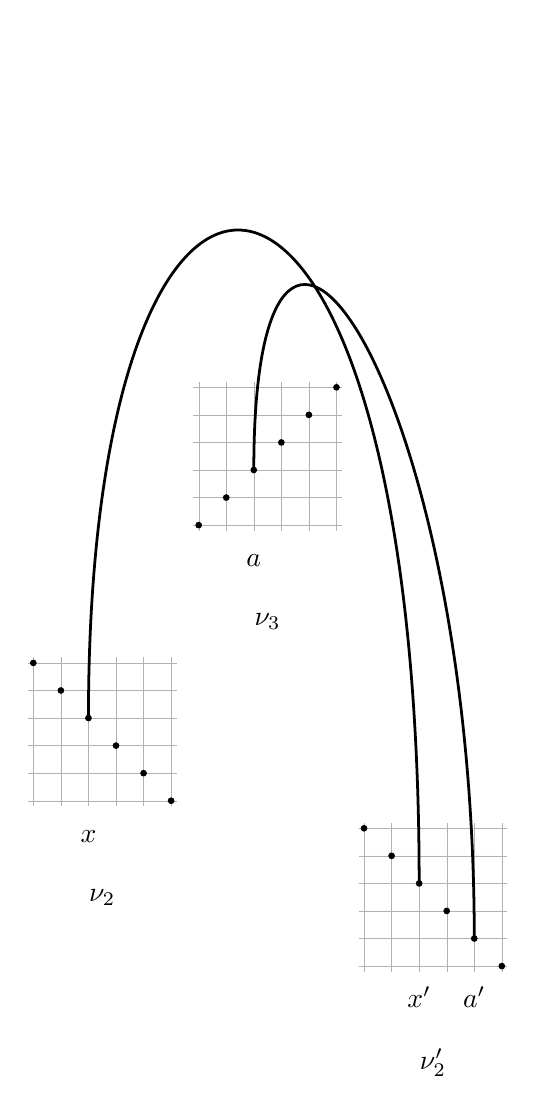
\begin{tikzpicture}
        [
          scale=0.35,
          label/.style={anchor=base}
        ]
        % nu_2
        \draw[step=1cm,black!30,ultra thin,fill=black!10] (-0.2,5.8) grid (5.2,11.2);
        \foreach \x/\y in {0/11,1/10,2/9,3/8,4/7,5/6} {
            \draw [fill=black] (\x,\y) circle (0.1);
        }
        % nu_3
        \draw[step=1cm,black!30,ultra thin,fill=black!10] (5.8,15.8) grid (11.2,21.2);
        \foreach \x/\y in {6/16,7/17,8/18,9/19,10/20,11/21} {
            \draw [fill=black] (\x,\y) circle (0.1);
        }
        % nu'_2
        \draw[step=1cm,black!30,ultra thin,fill=black!10] (11.8,-0.2) grid (17.2,5.2);

        \foreach \x/\y in {12/5,13/4,14/3,15/2,16/1,17/0} {
            \draw [fill=black] (\x,\y) circle (0.1);
        }
        % labels
        \node [label] (x) at (2,4.5) {$x$};
        \node [label] (a) at (8,14.5) {$a$};
        \node [label] (xp) at (14,-1.5) {$x'$};
        \node [label] (ap) at (16,-1.5) {$a'$};
        \node (nu1) at (2.5,2.5) {$\nu_2$};
        \node (nu2) at (8.5,12.5) {$\nu_3$};
        \node (nu1') at (14.5,-3.5) {$\nu'_2$};
        % crossings edges
        \draw [line width=1pt]
        (2,9) .. controls +(0,25) and +(0,30) .. (14,3);
        \draw [line width=1pt]
        (8,18) .. controls +(0,15) and +(0,20) .. (16,1);
      \end{tikzpicture}
    \caption{\label{fig:subfig:no (nu_3, nu'_2)-edge}%
      Claim~\ref{claim:no (nu_3, nu'_2)-edge}:
      Assuming a $(\nu_3, \nu'_2)$-edge $(a, b)$ in $\mathcal{M}$.
    }
  \end{figure}

  \begin{claim}
    \label{claim:no (nu_3, nu'_2)-edge}
    There is no $(\nu_3, \nu'_2)$-edge in $\mathcal{M}$.
  \end{claim}

  \begin{proof}[of Claim~\ref{claim:no (nu_3, nu'_2)-edge}]
    Suppose, aiming at a contradiction, that there exists
    $(\nu_3, \nu'_2)$-edge $(a, a')$ in $\mathcal{M}$.
    According to Claim~\ref{claim:(nu_2, nu'_2)-edge}, there
    exists at least one $(\nu_2, \nu'_2)$-edge $(x, x')$ in $\mathcal{M}$.
    Since $\mathcal{M}$ is containment-free (Lemma~\ref{lemma:matching}),
    we have $x' < a'$.
    Therefore,
    we have $\mu(x) < \mu(a)$ (since $\nu_2$ is below $\nu_3$) and
    $\mu(x') > \mu(a')$ (since $\nu'_2$ is decreasing),
    which contradicts our hypothesis about $\mathcal{M}$.
    See Fig.~\ref{fig:subfig:no (nu_3, nu'_2)-edge}.
    \qed
  \end{proof}

  \begin{claim}
    \label{claim:at most one (nu_2, nu_3)-edge}
    There is at most one $(\nu_2, \nu_3)$-edge
    in $\mathcal{M}$.
  \end{claim}

  \begin{proof}[of Claim~\ref{claim:at most one (nu_2, nu_3)-edge}]
    Apply Lemma~\ref{lemma:at most one edge monotone}.
    \qed
  \end{proof}

    We will see soon (upcoming Claim~\ref{claim:all (nu_2, nu'_2)-edges})
    that there exists actually no $(\nu_2, \nu_3)$-edge
    in $\mathcal{M}$.

  \begin{claim}
    \label{claim:no (nu_1, nu_3)-edge and no (nu'_1, nu_3)-edge}
    There is neither a $(\nu_1, \nu_3)$-edge not a $(\nu'_1, \nu_3)$-edge
    in $\mathcal{M}$.
  \end{claim}

 \begin{proof}[of Claim~\ref{claim:no (nu_1, nu_3)-edge and no (nu'_1, nu_3)-edge}]
    We first prove that there is no $(\nu_1, \nu_3)$-edge in $\mathcal{M}$.
    Indeed, suppose, aiming at a contradiction, that these exists
    a $(\nu_1, \nu_3)$-edge $(a, a')$ in $\mathcal{M}$.
    According to Claim~\ref{claim:(nu_1, nu'_1)-edge},
    there exists a $(\nu_1, \nu'_1)$-edge $(b, b')$ in $\mathcal{M}$.
    Since $\mathcal{M}$ is containment-free, we must have
    $b < a'$.
    Then it follows that
    $\mu(b) < \mu(a)$ (since $\nu_1$ is incresing) and
    $\mu(b') > \mu(a')$ (since $\nu'_1$ is above $\nu_3$),
    which contradicts our hypothesis about $\mathcal{M}$.

    As for no $(\nu_1, \nu_3)$-edges in $\mathcal{M}$, suppose,
    aiming at a contradiction, that these exists
    a $(\nu'_1, \nu_3)$-edge $(a, a')$ in $\mathcal{M}$.
    According to Claim~\ref{claim:(nu_1, nu'_1)-edge},
    there exists a $(\nu_1, \nu'_1)$-edge $(b, b')$ in $\mathcal{M}$.
    Then it follows that
    $\mu(b) < \mu(a)$ (since $\nu_1$ is below $\nu'_1$) and
    $\mu(b') > \mu(a')$ (since $\nu'_1$ is above $\nu_3$),
    which contradicts our hypothesis about $\mathcal{M}$.
    \qed
  \end{proof}

  \begin{claim}
    \label{claim:(nu_3, nu'_3)-edge}
    There exists a $(\nu_3, \nu'_3)$-edge in $\mathcal{M}$.
  \end{claim}

  \begin{proof}[of Claim~\ref{claim:(nu_3, nu'_3)-edge}]
    Suppose, aiming at a contradiction, that there is no
    $(\nu_3, \nu'_3)$-edge in $\mathcal{M}$.
    Combining
    Claim~\ref{claim:no edge below (nu_2, nu'_2)-edge},
    Claim~\ref{claim:no (nu_3, nu'_2)-edge},
    Claim~\ref{claim:at most one (nu_2, nu_3)-edge}
    and Claim~\ref{claim:no (nu_1, nu_3)-edge and no (nu'_1, nu_3)-edge},
    we conclude that $N_3-1$ positions in $\nu_3$ are involved
    in edges of $\mathcal{M}$ that are
    neither ($\nu_1, \nu_3)$-edges,
    nor $(\nu_2, \nu_3)$-edges
    nor $(\nu'_1, \nu_3)$-edges
    nor $(\nu_3, \nu_3)$-edges.
    But $N_3 - 1 > 2N_4 + 2n + 2k + 4$ (the positions left) and hence
    $\mathcal{M}$ is not a perfect matching,
    which contradicts our hypothesis about $\mathcal{M}$.
    \qed
  \end{proof}

  \begin{claim}
    \label{claim:no edge below one (nu_3, nu'_3)-edge}
    There is
    neither a $(\sigma', \sigma')$-edge,
    nor a $(\sigma', \nu_4)$-edge,
    nor a $(\sigma', \nu'_2)$-edge,
    nor a $(\nu_4, \nu_4)$-edge
    nor a $(\nu_4, \nu'_2)$-edge,
    nor a $(\nu'_2, \nu'_2)$-edge
    in $\mathcal{M}$.
  \end{claim}

  \begin{proof}[of Claim~\ref{claim:no edge below one (nu_3, nu'_3)-edge}]
    Combine Claim~\ref{claim:(nu_3, nu'_3)-edge} with the fact that
    $\mathcal{M}$ is containment-free.
    \qed
  \end{proof}

  The next two claims state that $\mathcal{M}$ actually contains
  all $(\nu_1, \nu'_1)$-edges and all $(\nu_2, \nu'_2)$-edges.

  \begin{claim}
    \label{claim:all (nu_1, nu'_1)-edges}
    $\mathcal{M}$ contains $N_1$ pairwise crossing $(\nu_1, \nu'_1)$-edges.
  \end{claim}

  \begin{proof}[of Claim~\ref{claim:all (nu_1, nu'_1)-edges}]
    Suppose, aiming at a contradiction, that
    $\mathcal{M}$ does not contain $N_1$ $(\nu_1, \nu'_1)$-edge.
    Combing Claim~\ref{claim:no (nu_2, nu'_1)-edge} and
    Claim~\ref{claim:no edge below (nu_2, nu'_2)-edge},
    we conclude that there exists a position $a$ in $\nu'_1$ that is
    involded in an edge $(a, a')$ in $\mathcal{M}$ that is
    neither a $(\nu_1, \nu'_1)$-edge,
    nor a $(\nu_2, \nu'_1)$-edge,
    nor a $(\nu'_1, \nu'_1)$-edge.
    (In other words, $a' > 2N_1 + N_2$.)
    Furthermore, according to Claim~\ref{claim:(nu_1, nu'_1)-edge},
    there exists a $(\nu_1, \nu'_1)$-edge $(x, x')$ in $\mathcal{M}$.
    Then, we have
    $\mu(x) < \mu(a)$ (since $\nu_1$ is below $\nu'_1$) and
    $\mu(x') < \mu(a')$ (since $\nu'_1$ is above any other gadget),
    which contradicts our hypothesis about $\mathcal{M}$.
    \qed
  \end{proof}

  \begin{claim}
    \label{claim:all (nu_2, nu'_2)-edges}
    $\mathcal{M}$ contains $N_2$ pairwise crossing $(\nu_2, \nu'_2)$-edges.
  \end{claim}

  \begin{proof}[of Claim~\ref{claim:all (nu_2, nu'_2)-edges}]
    The key idea is to focus on $\nu'_2$.
    Combining Claim~\ref{claim:no (nu_3, nu'_2)-edge},
    Claim~\ref{claim: no edge right of nu'_2} and
    Claim~\ref{claim:no edge below one (nu_3, nu'_3)-edge},
    we obtain that every position in $\nu'_2$ is involved in
    either a $(\nu_1, \nu'_2$)-edge
    or a $(\nu'_1, \nu'_2$)-edge
    or $(\nu_2, \nu'_2$)-edge.
    But, according to Claim~\ref{claim:all (nu_1, nu'_1)-edges},
    all positions in $\nu_1$ and $\nu'_1$ are involved in
    $(\nu_1, \nu'_1)$-edges.
    Then it follows that
    all positions in $\nu'_2$ are involved in a $(\nu_2, \nu'_2)$,
    and hence
    $\mathcal{M}$ contains $N_2$ pairwise crossing $(\nu_2, \nu'_2)$-edges.
    \qed
  \end{proof}

  \begin{claim}
    \label{claim:no (nu_2, nu_4)-edge}
    There is no $(\nu_2, \nu_4)$-edge in $\mathcal{M}$.
  \end{claim}

  \begin{proof}[of Claim~\ref{claim:no (nu_2, nu_4)-edge}]
    According to Claim~\ref{claim:all (nu_2, nu'_2)-edges},
    all positions in $\nu_2$ and $\nu'_2$ are involved in
    $(\nu_2, \nu'_2)$-edges in $\mathcal{M}$.
    \qed
  \end{proof}

  \begin{claim}
    \label{claim:no (nu_4, nu'_3)-edge}
    There is no $(\nu_4, \nu'_3)$-edge in $\mathcal{M}$.
  \end{claim}

  \begin{proof}[of Claim~\ref{claim:no (nu_4, nu'_3)-edge}]
    Suppose, aiming at a contradiction, that there exists
    a $(\nu_4, \nu'_3)$-edge $(a, a')$ in $\mathcal{M}$.
    According to Claim~\ref{claim:(nu_3, nu'_3)-edge},
    there exists a $(\nu_3, \nu'_3)$-edge $(x, x')$
    in $\mathcal{M}$.
    Since $\mathcal{M}$ is containment-free, we must have
    $x' < a'$.
    Therefore,
    we have $\mu(x) > \mu(a)$ (since $\nu_3$ is above $\nu_4$) and
    $\mu(x') < \nu(a')$ (since $\nu'_3$ is increasing),
    which contradicts our hypothesis about $\mathcal{M}$.
    \qed
  \end{proof}

  \begin{claim}
    \label{claim:(nu_4, nu'_4)-edge}
    There is at least one $(\nu_4, \nu'_4)$-edge in $\mathcal{M}$.
  \end{claim}

  \begin{proof}[of Claim~\ref{claim:(nu_4, nu'_4)-edge}]
    Suppose, aiming at a contradiction, that there is no
    $(\nu_4, \nu'_4)$-edge in $\mathcal{M}$.
    First, according to
    Claim~\ref{claim:all (nu_1, nu'_1)-edges} and
    Claim~\ref{claim:all (nu_2, nu'_2)-edges},
    there is neither a $(\nu_1, \nu_4)$-edge
    nor a $(\nu'_1, \nu_4)$-edge
    nor a $(\nu_2, \nu_4)$-edge
    nor a $(\nu_4, \nu'_2)$-edge in $\mathcal{M}$.
    Furthermore, according to
    Claim~\ref{claim:no edge below (nu_2, nu'_2)-edge} and
    Claim~\ref{claim:no (nu_4, nu'_3)-edge},
    there is neither a $(\nu_3, \nu_4)$-edge
    nor a $(\nu_4, \nu'_3)$-edge in $\mathcal{M}$.
    But $N_4 > 2n + 2k + 2$, and
    hence $\mathcal{M}$ is not perfect,
    which contradicts our hypothesis about $\mathcal{M}$.
    \qed
  \end{proof}

  \begin{claim}
    \label{claim:no edge below (nu_4, nu'_4)-edge}
    There is
    neither a $(\pi', \pi')$-edge
    nor a $(\sigma', \pi'')$-edge
    nor a $(\sigma', \sigma'')$-edge
    in $\mathcal{M}$.
  \end{claim}

  \begin{proof}[of Claim~\ref{claim:no edge below (nu_2, nu'_2)-edge}]
    Combine Claim~\ref{claim:(nu_4, nu'_4)-edge} with the
    fact that $\mathcal{M}$ is containment-free.
    \qed
  \end{proof}

  \begin{claim}
    \label{claim:no (sigma', nu'_3)-edge, no (sigma', nu'_4)-edge}
    There is neither a $(\sigma', \nu'_3)$-edge
    nor a $(\sigma', \nu'_4)$-edge in $\mathcal{M}$.
  \end{claim}

  \begin{proof}[of Claim~\label{claim:no (sigma', nu'_3)-edge}]
    According to
    Claim~\ref{claim: no edge right of nu'_2},
    Claim~\ref{claim:all (nu_1, nu'_1)-edges}
    Claim~\ref{claim:all (nu_2, nu'_2)-edges} and
    Claim~\ref{claim:no (nu_4, nu'_3)-edge}
    every position in $\sigma'$ is involved in
    either a $(\sigma', \nu'_3)$-edge
    or a $(\sigma', \pi')$-edge
    or a $(\sigma', \nu'_4)$-edge
    in $\mathcal{M}$.
    Let $a$ be the first position of $\sigma'$
    (\emph{i.e.}, $a = 2N_1 + N_2 + N_3 + 1$)
    and
    $b$ be the last position of $\sigma'$
    (\emph{i.e.}, $b = 2N_1 + N_2 + N_3 + k + 2$),
    and write $(a, a')$ and $(b, b')$ for the two associated edges of $\mathcal{M}$.
    We consider the presence of a $(\sigma', \nu'_3)$-edge
    or a $(\sigma', \nu'_4)$-edge in $\mathcal{M}$ separately.
    \begin{itemize}
      \item
      Suppose, aiming at a contradiction, that there exists
      a $(\sigma', \nu'_3)$-edge in $\mathcal{M}$.
      Since $\mathcal{M}$ is containment-free, we conclude that
      $(a, a')$ must be a $(\sigma', \nu'_3)$-edge.
      But $\mu(a) = 2N_2 + N_4 + 2n + k + 2 + (k+1) <
      \mu(b) = 2N_2 + N_4 + 2n + k + 2 + (k+2)$, and hence
      $(b, b')$ is also a $(\sigma', \nu'_3)$-edge
      (otherwise we would have $\mu(a') > \mu(b')$ since
      $\nu'_3$ is above $\pi'$ and $\nu'_4$,
      which contradicts our hypothesis).
      Consider any position $c$ but $a$ and $b$ of $\sigma'$
      (\emph{i.e.},
      $a = 2N_1 + N_2 + N_3 + 1 < c < 2N_1 + N_2 + N_3 + k + 2 = b$),
      and let $(c, c')$ be the associate edge in $\mathcal{M}$.
      We first observe that $(c, c')$ is not a $(\sigma', \nu'_3)$-edge,
      since otherwise we would have
      $\mu(a) > \mu(c)$ and $\mu(a') < \mu(c')$
      (since $\mathcal{M}$ is containment-free and $\nu'_3$ is increasing),
      thereby contradicting our hypothesis about $\mathcal{M}$.
      Therefore, $(c, c')$ is either a $(\sigma', \pi)$-edge or a $(\sigma', \nu'_4)$-edge.
      In both cases, $(b, b')$ is contained in $(c, c')$,
      which contradicts our hypothesis about $\mathcal{M}$ being containment-free.
      \item
      Suppose, aiming at a contradiction, that there exists
      a $(\sigma', \nu'_4)$-edge in $\mathcal{M}$.
      Since $\mathcal{M}$ is containment-free, we conclude that
      $(b, b')$ must be a $(\sigma', \nu'_4)$-edge.
      Since there is no $(\sigma', \nu'_3)$-edge in $\mathcal{M}$
      (preceding point),
      $(a, a')$ is either a
      $(\sigma', \pi')$-edge or a $(\sigma', \nu'_4)$-edge.
      In both cases, we have $a' < a$.
      Then it follows that
      $\mu(a) < \mu(b)$
      (since $2N_2 + N_4 + 2n + k + 2 + (k+1) < 2N_2 + N_4 + 2n + k + 2 + (k+2)$)
      and
      $\mu(a') > \mu(b')$ (since $\pi'$ is above $\nu'_4$ if $(a, a')$ is
      a $(\sigma', \pi')$-edge and
      $\nu'_4$ is decreasing if $(a, a')$ is
      a $(\sigma', \nu'_4)$-edge),
      which contradicts our hypothesis about $\mathcal{M}$.
    \end{itemize}
    \qed
  \end{proof}

  Combining the above claims, we conclude that there are
  $k+2$ $(\sigma', \pi')$-edges in $\mathcal{M}$.
  Recall that
  $\sigma' = ((k+1) \; \sigma \; (k+2)) \; [2N_2 + N_4 + 2n + k + 2]$ and that
  $\pi' = ((n+1) \; \pi \; (n+2)) \; [2N_2 + N_4 + n + k + 2]$.
  Then it follows we have
  at least $k$ (possibly $k+1$ or $k+2$) independent $(\sigma', \pi')$-edges
  $(a, a')$ in $\mathcal{M}$ with
  $2N_1 + N_2 + N_3 + 1 < a < 2N_1 + N_2 + N_3 + k + 2$
  and
  $2N_1 + N_2 + N_3 + (k + 2) + 1 < a' < 2N_1 + N_2 + N_3 + (k + 2) + n + 2$.
  Therefore, by our hypothesis about $\mathcal{M}$,
  $\sigma$ occurs as a pattern in $\pi$.
  \qed
\end{proof}

%%%%%%%%%%%%%%%%%%%%%%%%%%%%%%%%%%%%%%%%%%%%%%%%%%%%%%%%%%%%%%%%%%%%

% %%
% %% ---- Patterns ----
% %%
% \section{Patterns}
% \label{section:Patterns}
%
% \begin{proposition}
%   \label{proposition:patterns:lower bound}
%   Let $\pi \in S_{n}$.
%   Then $\pi$ contains a pattern of size at least
%   $\left\lfloor\sqrt{n-1}/2\right\rfloor$ that
%   is the union of two order-isomorphic patterns.
% \end{proposition}
%
% \begin{proof}[of Proposition~\ref{proposition:patterns:lower bound}]
%   The Erdös-Szekeres theorem \cite{Erdos:Szekeres:1935}
%   states that every permutation of
%   length at least $pq+1$ must contain either the pattern
%   $\nearrow_{p+1}$ or the pattern $\searrow_{q+1}$.
%   The result now follows from the fact that
%   the pattern $\nearrow_{p+1}$ (resp. $\searrow_{q+1}$)
% \qed
% \end{proof}
%
% \begin{proposition}
%   \label{proposition:patterns:upper bound}
%   If $2^{\binom{k}{2}} > \binom{n}{2k}\;\binom{2k}{k}$, then there exists
%   a permutation of $S_{n}$
%   that does not contains a pattern
%   of length $2k$ that is the union of two
%   order-isomorphic patterns.
% \end{proposition}
%
% \begin{proof}[of Proposition~\ref{proposition:patterns:upper bound}]
% The proof is by the probabilistic method \cite{Alon:Spencer:1992}.
% Let $\pi \in S_n$ be chosen randomly and uniformly.
% For any pattern $\sigma$ of length $2k$ ($k$ to be precisely defined latter)
% of $\pi$,
% let $X_\sigma$ be the indicator variable that
% $\sigma$ is the union of two order-ismorphic patterns.
% According to Boole's inequality, we have
% $P\left(X_\sigma\right) \leq \binom{2k}{k}\;2^{-k}$.
% Since there are $\binom{n}{2k}$ patterns of length $2k$ in $\pi$,
% the probability that $\pi$ contains a pattern of length $2k$
% is the union of two order-ismorphic patterns is at most
% $\binom{n}{2k}\;\binom{2k}{k}\;2^{-k} < 1$.
% Thus, with positive probability, no event $X_\sigma$ occurs and
% there is a permutation of $S_n$ that does not contain a pattern
% of length $2k$ that is the union of two order-isomorphic patterns.
% \qed
% \end{proof}

%%%%%%%%%%%%%%%%%%%%%%%%%%%%%%%%%%%%%%%%%%%%%%%%%%%%%%%%%%%%%%%%%%%%

%%
%% ---- Conclusion ----
%%
\section{Conclusion}
\label{section:Conclusion}

There are a number of further directions of investigation in this
general subject. We mention several -~not necessarily new~- open
problems that are, in our opinion, the most interesting. How many
permutations of $S_{2n}$ are squares? How many $(213,231)$-avoiding
permutations of $S_{2n}$ are squares? (Equivalently, by
Proposition~\ref{prop:bijection_binary_to_permutations_squares},
how many binary strings of length $2n$ are squares; Problem~4
in \cite{Henshall:Rampersad:Shallit:2011})? How hard is the problem of
deciding whether a $(213,231)$-avoiding permutation is a square
(Problem~4 in \cite{Henshall:Rampersad:Shallit:2011},
see also \cite{Buss:Soltys:2014,Rizzi:Vialette:CSR:2013})?
Given two permutations $\pi$ and $\sigma$, how hard is the problem of
deciding whether $\sigma$ is a square root of $\pi$?
\smallskip

Besides, in this work, we investigate some algebraic properties of the
shuffle of permutations which have direct combinatorial consequences.
However, this work raises several additional classical algebraic
questions. Among these, one can ask for a complete algebraic study of
$\QQ[S]$ as a graded associative algebra for the shuffle  product
$\SHUFFLE$. Describing a generating family for $\QQ[S]$, defining
multiplicative bases of $\QQ[S]$, and determining whether $\QQ[S]$ is
free as an associative algebra are worthwhile questions.

%%%%%%%%%%%%%%%%%%%%%%%%%%%%%%%%%%%%%%%%%%%%%%%%%%%%%%%%%%%%%%%%%%%%

%%
%% Bibliography
%%

\bibliographystyle{plain}
\bibliography{biblio}

%%%%%%%%%%%%%%%%%%%%%%%%%%%%%%%%%%%%%%%%%%%%%%%%%%%%%%%%%%%%%%%%%%%%%%%%%%%%%%%

\newpage
\section*{Appendix (Reviewers' version only)}


%%%%%%%%%%%%%%%%%%%%%%%%%%%%%%%%%%%%%%%%%%%%%%%%%%%%%%%%%%%%%%%%%%%%%%%%%%%%%%%

\end{document}

%%%%%%%%%%%%%%%%%%%%%%%%%%%%%%%%%%%%%%%%%%%%%%%%%%%%%%%%%%%%%%%%%%%%%%%%%%%%%%%
